\PassOptionsToPackage{svgnames}{xcolor}
\documentclass[12pt,francais,]{scrbook}
\usepackage{lmodern}
\usepackage{wallpaper}
\usepackage{amssymb,amsmath}
\usepackage{xcolor}
\definecolor{ocre}{RGB}{243,102,25}
\usepackage{ifxetex,ifluatex}
\usepackage{fixltx2e} % provides \textsubscript
% use upquote if available, for straight quotes in verbatim environments
\IfFileExists{upquote.sty}{\usepackage{upquote}}{}
\ifnum 0\ifxetex 1\fi\ifluatex 1\fi=0 % if pdftex
  \usepackage[T1]{fontenc}
  \usepackage[utf8]{inputenc}
\else % if luatex or xelatex
  \ifxetex
    % This will have to be removed some day : http://tex.stackexchange.com/questions/269786/unicode-math-broken
    \expandafter\let\csname xetex_suppressfontnotfounderror:D\endcsname
      \suppressfontnotfounderror
    \usepackage{mathspec}
    \usepackage{xltxtra,xunicode}
  \else
    \usepackage{fontspec}
  \fi
  \defaultfontfeatures{Mapping=tex-text,Scale=MatchLowercase}
  \newcommand{\euro}{€}
    \setmainfont{Merriweather}
    \setmonofont[Mapping=tex-ansi]{Andale Mono}
\fi
% use microtype if available
\IfFileExists{microtype.sty}{\usepackage{microtype}}{}
\usepackage[margin=1in]{geometry}
\usepackage{color}
\usepackage{fancyvrb}
\newcommand{\VerbBar}{|}
\newcommand{\VERB}{\Verb[commandchars=\\\{\}]}
\DefineVerbatimEnvironment{Highlighting}{Verbatim}{commandchars=\\\{\}}
% Add ',fontsize=\small' for more characters per line
\newenvironment{Shaded}{}{}
\newcommand{\KeywordTok}[1]{\textcolor[rgb]{0.00,0.44,0.13}{\textbf{{#1}}}}
\newcommand{\DataTypeTok}[1]{\textcolor[rgb]{0.56,0.13,0.00}{{#1}}}
\newcommand{\DecValTok}[1]{\textcolor[rgb]{0.25,0.63,0.44}{{#1}}}
\newcommand{\BaseNTok}[1]{\textcolor[rgb]{0.25,0.63,0.44}{{#1}}}
\newcommand{\FloatTok}[1]{\textcolor[rgb]{0.25,0.63,0.44}{{#1}}}
\newcommand{\ConstantTok}[1]{\textcolor[rgb]{0.53,0.00,0.00}{{#1}}}
\newcommand{\CharTok}[1]{\textcolor[rgb]{0.25,0.44,0.63}{{#1}}}
\newcommand{\SpecialCharTok}[1]{\textcolor[rgb]{0.25,0.44,0.63}{{#1}}}
\newcommand{\StringTok}[1]{\textcolor[rgb]{0.25,0.44,0.63}{{#1}}}
\newcommand{\VerbatimStringTok}[1]{\textcolor[rgb]{0.25,0.44,0.63}{{#1}}}
\newcommand{\SpecialStringTok}[1]{\textcolor[rgb]{0.73,0.40,0.53}{{#1}}}
\newcommand{\ImportTok}[1]{{#1}}
\newcommand{\CommentTok}[1]{\textcolor[rgb]{0.38,0.63,0.69}{\textit{{#1}}}}
\newcommand{\CommentTokAlt}[1]{\textcolor[rgb]{0.18,0.33,0.39}{\textit{{#1}}}}
\newcommand{\DocumentationTok}[1]{\textcolor[rgb]{0.73,0.13,0.13}{\textit{{#1}}}}
\newcommand{\AnnotationTok}[1]{\textcolor[rgb]{0.38,0.63,0.69}{\textbf{\textit{{#1}}}}}
\newcommand{\CommentVarTok}[1]{\textcolor[rgb]{0.38,0.63,0.69}{\textbf{\textit{{#1}}}}}
\newcommand{\OtherTok}[1]{\textcolor[rgb]{0.00,0.44,0.13}{{#1}}}
\newcommand{\FunctionTok}[1]{\textcolor[rgb]{0.02,0.16,0.49}{{#1}}}
\newcommand{\VariableTok}[1]{\textcolor[rgb]{0.10,0.09,0.49}{{#1}}}
\newcommand{\ControlFlowTok}[1]{\textcolor[rgb]{0.00,0.44,0.13}{\textbf{{#1}}}}
\newcommand{\OperatorTok}[1]{\textcolor[rgb]{0.40,0.40,0.40}{{#1}}}
\newcommand{\BuiltInTok}[1]{{#1}}
\newcommand{\ExtensionTok}[1]{{#1}}
\newcommand{\PreprocessorTok}[1]{\textcolor[rgb]{0.74,0.48,0.00}{{#1}}}
\newcommand{\AttributeTok}[1]{\textcolor[rgb]{0.49,0.56,0.16}{{#1}}}
\newcommand{\RegionMarkerTok}[1]{{#1}}
\newcommand{\InformationTok}[1]{\textcolor[rgb]{0.38,0.63,0.69}{\textbf{\textit{{#1}}}}}
\newcommand{\WarningTok}[1]{\textcolor[rgb]{0.38,0.63,0.69}{\textbf{\textit{{#1}}}}}
\newcommand{\AlertTok}[1]{\textcolor[rgb]{1.00,0.00,0.00}{\textbf{{#1}}}}
\newcommand{\ErrorTok}[1]{\textcolor[rgb]{1.00,0.00,0.00}{\textbf{{#1}}}}
\newcommand{\NormalTok}[1]{{#1}}
\usepackage{longtable,booktabs}
\usepackage{graphicx}
% Redefine \includegraphics so that, unless explicit options are
% given, the image width will not exceed the width of the page.
% Images get their normal width if they fit onto the page, but
% are scaled down if they would overflow the margins.
\makeatletter
\def\ScaleIfNeeded{%
  \ifdim\Gin@nat@width>\linewidth
    \linewidth
  \else
    \Gin@nat@width
  \fi
}
\makeatother
\let\Oldincludegraphics\includegraphics
{%
 \catcode`\@=11\relax%
 \gdef\includegraphics{\@ifnextchar[{\Oldincludegraphics}{\Oldincludegraphics[width=\ScaleIfNeeded]}}%
}%
\ifxetex
  \usepackage[setpagesize=false, % page size defined by xetex
              unicode=false, % unicode breaks when used with xetex
              xetex]{hyperref}
\else
  \usepackage[unicode=true]{hyperref}
\fi
\hypersetup{breaklinks=true,
            bookmarks=true,
            pdfauthor={14 décembre 2017},
            pdftitle={INTRODUCTION TO C PROGRAM PROOF USING FRAMA-C AND ITS WP PLUGIN},
            colorlinks=true,
            citecolor=ocre,
            urlcolor=ocre,
            linkcolor=magenta,
            pdfborder={0 0 0}}
\urlstyle{same}  % don't use monospace font for urls
\setlength{\parindent}{0pt}
\setlength{\parskip}{6pt plus 2pt minus 1pt}
\setlength{\emergencystretch}{3em}  % prevent overfull lines
\providecommand{\tightlist}{%
  \setlength{\itemsep}{0pt}\setlength{\parskip}{0pt}}
\setcounter{secnumdepth}{5}
\ifxetex
  \usepackage[english]{babel}
\else
  \usepackage[english]{babel}
\fi

\usepackage{tcolorbox}
\tcbuselibrary{skins,breakable}
\usetikzlibrary{shadings,shadows}

\newenvironment{zdsexampleblock}[1]{%
  \tcolorbox[beamer,%
    noparskip,breakable,
    colback=LightGreen,colframe=DarkGreen,%
    colbacklower=LimeGreen,%
    title=#1]
}{\endtcolorbox}

\newenvironment{zdsalertblock}[1]{%
  \tcolorbox[beamer,%
    noparskip,breakable,
    colback=LightCoral,colframe=DarkRed,%
    colbacklower=Tomato,%
    title=#1]
}{\endtcolorbox}

\newenvironment{zdssecretblock}[1]{%
  \tcolorbox[beamer,%
    noparskip,breakable,
    colback=LightGray,colframe=DarkGray,%
    colbacklower=LightGray,%
    title=#1]
}{\endtcolorbox}

\newenvironment{zdsblock}[1]{%
  \tcolorbox[beamer,%
    noparskip,breakable,
    colback=LightBlue,colframe=DarkBlue,%
    colbacklower=DarkBlue,%
    title=#1]
}{\endtcolorbox}

\usepackage{titlesec} % Allows customization of titles
\usepackage{graphicx} % Required for including pictures
\newcommand{\gt}{>}
\newcommand{\lt}{<}

\begin{titlepage}
\title{\color{white}{INTRODUCTION TO C PROGRAM PROOF USING FRAMA-C AND ITS WP PLUGIN}}
\author{\color{ocre}{Allan Blanchard}}
\date{\color{white}{$ $\\December 2017}}
\end{titlepage}

\graphicspath{{../../resources/}}

\begin{document}
\ULCornerWallPaper{1}{../../resources/coverpage.pdf}
\maketitle
\ClearWallPaper

{
\hypersetup{linkcolor=ocre}
\setcounter{tocdepth}{2}
\tableofcontents
}
\chapter{Introduction}\label{introduction}

\begin{zdsalertblock}
  Please note that this document is the very first english version of the
  tutorial. If you find some errors, please do not hesitate to contribute at:

  \href{https://github.com/AllanBlanchard/tutoriel_wp}{https://github.com/AllanBlanchard/tutoriel\_wp}

  Please use the markdown files, the LaTeX file being generated from them.
\end{zdsalertblock}

\begin{zdsblock}{Information}
  In this tutorial, some examples and some elements of organization are
  similar to the ones used in the \href{http://www.spacios.eu/TAP2013/keynotes.html}{TAP 2013
    tutorial} by Nikolai Kosmatov, Virgile Prevosto and Julien
  Signoles of the CEA LIST, since it is quite didactic. It also
  contains examples taken from
  \emph{\href{http://www.fokus.fraunhofer.de/download/acsl_by_example}{ACSL By Example}}
  by Jochen Burghardt, Jens Gerlach, Kerstin Hartig, Hans Pohl and Juan
  Soto from the Fraunhofer. The remaining ideas come from my personal
  experience with Frama-C and WP. The only requirement to this tutorial
  is to have a basic knowledge of the C language, and at least to
  be familiar with the notion of pointer.
\end{zdsblock}

Despite its old age, C is still a widely used programming language.
Indeed, no other language can pretend to be available on so many
different (hardware and software) platforms, its low-level orientation
and the amount of time invested in the optimization of its compilers
allows to generate very light and efficient machine code (if the code
allows it of course), and that there are a lot of experts in C language,
which is an important knowledge base.

Furthermore, a lot of systems rely on a huge amount of code historically
written in C, that needs to be maintained and sometimes fixed, as it
would be far too costly to rewrite these systems.

But anyone who has already developed with C also know that it is very
hard to perfectly master this language. There are numerous reasons, but
ambiguities in the ISO C, and the fact that it is extremely permissive,
especially about memory management, make the development of robust C
program very hard, even for an experienced programmer.

However, the C language is often chosen for critical systems (avionics,
railway, armament, \ldots{}) where it is appreciated for its good
performances, its technological maturity and the predictability of its
compilation.

In such cases, the needs in term of code covering by tests become
important. The question ``is our software tested enough?'' becomes a
question to which it is very hard to answer. Program proof can help us.
Rather than test all possible and (un)imaginable inputs to the program,
we will \emph{mathematically} prove that there cannot be any problem at
runtime.

The goal of this tutorial is to use Frama-C, a tool developed at the CEA
LIST, and WP, its deductive proof plugin, to learn the basics about C
program proof. More than the use of the tool itself, the goal of this
tutorial is to convince that it is more and more possible to write
programs without any programming error, but also to sensitize to simple
notions that allows to better understand and write programs.

\begin{zdsblock}{Information}
  Many thanks to the different beta-testers for their constructives
  feedback:
  \begin{itemize}
  \item \href{https://zestedesavoir.com/membres/voir/Taurre/}{Taurre} (the
    example in the section III - 3 - 4 has been shamefully ripped
    off from one of his posts)
  \item \href{https://zestedesavoir.com/membres/voir/barockobamo/}{barockobamo}
  \item \href{https://zestedesavoir.com/membres/voir/Vayel/}{Vayel}
  \end{itemize}
  I thank ZesteDeSavoir validators who helped me improve again the quality of
  this tutorial:
  \begin{itemize}
  \item \href{https://zestedesavoir.com/membres/voir/Taurre/}{Taurre} (again)
  \item \href{https://zestedesavoir.com/membres/voir/Saroupille/}{Saroupille}
  \end{itemize}
  Finally, many thanks to Jens Gerlach for his help during the translation of
  this tutorial from french to english.
\end{zdsblock}

\chapter{Program proof and our tool for this tutorial:
Frama-C}\label{program-proof-and-our-tool-for-this-tutorial-frama-c}

The goal of this first part is, in the first section, to introduce the
idea of program proof without giving to much details, and then, in the
second section, we will give the necessary instructions to install
Frama-C and some automatic provers that we will use in this tutorial.

\section{Program proof}\label{program-proof}

\subsection{Ensure program
reliability}\label{ensure-program-reliability}

It is often difficult to ensure that our programs have only correct
behaviors. Moreover, it is already complex to establish a good criteria
that makes us confident enough to say that a program correctly works:

\begin{itemize}
\tightlist
\item
  beginners simply ``try'' to use their programs and considers that
  these programs work if they do not crash (which is not a really good
  indicator in C language),
\item
  more advanced developers establish some test cases for which they know
  the expected result and compare the output they obtain,
\item
  most of companies establish complete test bases, that covers as much
  code as they can ; which are systematically executed on their code.
  Some of them apply test driven development,
\item
  in critical domains, such as aerospace, railway or armament, every
  code needs to be certified using standardized processes with very
  strict criteria about coding rules and code covering by the test.
\end{itemize}

In all these ways to ensure that a program produces only what we expect
it to produce, a word appears to be common: \emph{test}. We \emph{try}
different inputs in order to isolate cases that are problematic. We
provide inputs that we \emph{estimate to be representative} of the
actual use of the program (note that unexpected use case are often not
considered whereas there are generally the most dangerous ones) and we
verify that the results we get are correct. But we cannot test
\emph{everything}. We cannot try \emph{every} combination of
\emph{every} possible input of a program. It is then quite hard to
choose good tests.

The goal of program proof is to ensure that, for any input provided to a
given program, if it respects the specification, then the program will
only well-behave. However, since we cannot test everything, we will
formally, mathematically, establish a proof that our software can only
exhibit specified behaviors, and that runtime-errors are not part of
these behaviors.

A very well-known quote from Dijkstra precisely express the difference
between test and proof :

\begin{quote}
Program testing can be used to show the presence of bugs, but never to
show their absence! \hfill {[}Dijkstra{]}
\end{quote}

\subsubsection{The developer's Holy Grail: the bug-free
software}\label{the-developers-holy-grail-the-bug-free-software}

Every time we can read news about attacks on computer systems, or
viruses, or bugs leading to crashes in well known apps, there is always
the one same comment ``the bug-free/perfectly secure program does not
exist''. And, if this sentence is quite true, it is a bit misunderstood.

Apart from the difference between safety and security (that we can very
vaguely define by the existence of a malicious entity), we do not really
define what we mean by ``bug-free''. Creating software always rely at
least on two steps: we establish a specification of what we expect from
the program and then we produce the source code of the program that must
respect this specification. Both of these steps can lead to the
introduction of errors.

In this tutorial, we will show how we can prove that an implementation
verify a given specification. But what are the arguments of program
proof, compared to program testing? First, the proof is complete, it
cannot forget some corner case if the behavior is specified (program
test cannot be complete, being exhaustive would be far too costly).
Then, the obligation to formally specify with a logic formulation
requires to exactly understand what we have to prove about our program.

One could cynically say that program proofs shows that ``the
implementation does not contain bugs that do not exist in the
specification''. But, well, it is already a big step compared to ``the
implementation does not contain too many bugs that do not exist in the
specification''. Moreover, there also exist approaches that allow to
analyze specifications to find errors or under-specified behaviors. For
example, with model checking techniques, we can create an abstract model
from the specification and produce the set of states that can be reach
according to this model. By characterizing what is an error state, we
can determine if reachable states are error states.

\subsection{A bit of context}\label{a-bit-of-context}

Formal methods, as we name them, allow in computer science to
rigorously, mathematically, reason about programs. There exist a lot of
formal methods that can take place at different levels from program
design to implementation, analysis and validation, and for all system
that allow to manipulate information.

Here, we will focus on a method that allows to formally verify that our
programs have only correct behaviors. We will use tools that are able to
analyze a source code and to determine whether a program correctly
implements what we want to express. The analyzer we will use provides a
static analysis, that we can oppose to dynamic analysis.

In static analysis, the analyzed program is not executed, we reason on a
mathematical model of the states it can reach during its execution. On
the opposite, dynamic analyses such as program testing, require to
execute the analyzed source code. Note that there exist formal dynamic
analysis methods, for example automatic test generation, or code
monitoring techniques that allows to instrument a source code to verify
some properties about it during execution (correct memory use, for
example).

Talking about static analyses, the model we use can be more or less
abstract depending on the techniques, it is always an approximation of
possible states of the program. The more the approximation is precise,
the more the model is concrete, the more the approximation is vague, the
more it is abstract.

To illustrate the difference between concrete and abstract model, we can
have a look to the model of simple chronometer. A very abstract model of
a chronometer could be the one presented in Figure~\ref{fig:1-1-chrono}.

\begin{figure}[htbp]
\centering
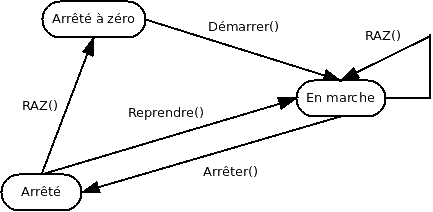
\includegraphics[scale=0.5]{1-1-model.png}
\caption{A very abstract model of a chronometer}
\label{fig:1-1-chrono}
\end{figure}

We have a model of the behavior of our chronometer with the different
states it can reach according to the different actions we can perform.
However, we do not have modeled how these states are depicted inside the
program (is this a C enumeration? a particular program point in the
source code?), nor how is modeled the time computation (a single
variable? multiple ones?). It would then be difficult to specify
properties about our program. We could add some information:

\begin{itemize}
\tightlist
\item
  State stopped at 0 : time = 0s
\item
  State running : time \textgreater{} 0s
\item
  State stopped : time \textgreater{} 0s
\end{itemize}

Which gives us a more concrete model but that is still not precise
enough to ask interesting questions like: ``is it possible to be in the
state stopped and that time is still updated?'', as we do not model how
the time measurement is updated by the chronometer.

On the opposite, with the source code of the program, we have a concrete
model of the chronometer. The source code expresses the behavior of the
chronometer since it will allow us to produce the executable. But this
is still not the more concrete model! For example, the executable in
machine code format, that we obtain after compilation, is far more
concrete than our program.

The more a model is concrete, the more it precisely describes the
behavior of our program. The source code more precisely describes the
behavior than our diagram, but it is less precise than the machine code.
However, the more the model is precise, the more it is difficult to have
a global view of the defined behavior. Our diagram is understandable in
a blink of an eye, the source code requires more time, and for the
executable \ldots{} Every single person that has already opened an
executable with a text editor by error knows that it is not really
pleasant to read\footnote{There also exists formal methods which are
  interested in understanding how executable machine code work, for
  example in order to understand what malwares do or to detect security
  breaches introduced during compilation.}.

When we create an abstraction of a system, we approximate it, in order
to limit the knowledge we have about it and ease our reasoning. A
constraint we must respect, if we want our analysis to be correct, is to
never under-approximate behaviors: we would risk to remove a behavior
that contains an error. However, when we over-approximate it, we can add
behaviors that cannot happen, and if we add to many of them, we could
not be able to prove our program is correct, since some of them could be
faulty behaviors.

In our case, the model is quite concrete. Every type of instruction, of
control structure, is associated to a precise semantics, a model of its
behavior in a pure logic, mathematical, world. The logic we use here is
a variant of the Hoare logic, adapted to the C language and all its
complex subtleties (which makes this model concrete).

\subsection{Hoare triples}\label{hoare-triples}

Hoare logic is a program formalization method proposed by Tony Hoare in
1969 in a paper entitled \emph{An Axiomatic Basis for Computer
Programming}. This method defines:

\begin{itemize}
\tightlist
\item
  axioms, that are properties we admit, such as ``the skip action does
  not change the program state'',
\item
  rules to reason about the different allowed combinations of actions,
  for example ``the skip action followed by the action A'' is equivalent
  to ``the action A''.
\end{itemize}

The behavior of the program is defined by what we call ``Hoare
triples'':

\begin{center} \(\{P\} C \{Q\}\) \end{center}

Where \(P\) and \(Q\) are predicates, logic formulas that express
properties about the memory at particular program points. \(C\) is a
list of instructions that defines the program. This syntax expresses the
following idea: ``if we are in a state where \(P\) is verified, after
executing \(C\) and if \(C\) terminates, then \(Q\) is verified for the
new state of the execution''. Put in another way, \(P\) is a sufficient
precondition to ensure that \(C\) will bring us to the postcondition
\(Q\). For example, the Hoare triples that corresponds to the skip
action is the following one:

\begin{center} \(\{P\}\) \textbf{skip} \(\{P\}\) \end{center}

When we do nothing, the postcondition is the precondition.

Along this tutorial, we will present the semantics of different program
constructs (conditional blocks, loops, etc) using Hoare logic. So, we
will not enter into details now since we will work on it later. It is
not necessary to memorize these notions nor to understand all the
theoretical background, but it is still useful to have some ideas about
the way our tool works.

All of this gives us the basics that allows us to say ``here is what
this action does'' but it does not give us anything to mechanize a
proof. The tool we will use rely on a technique called weakest
precondition calculus.

\subsection{Weakest precondition
calculus}\label{weakest-precondition-calculus}

The weakest precondition calculus is a form of predicate transform
semantics proposed by Dijkstra in 1975 in \emph{Guarded commands,
non-determinacy and formal derivation of programs}.

This sentence can appear complex but the actual meaning is in fact quite
simple. We have seen before that Hoare logic gives us rules that explain
the behavior of the different actions of a program, but it does not say
how to apply these rules to establish a complete proof of the program.

Dijkstra reformulate the Hoare logic by explaining, in the triple
\(\{P\}C\{Q\}\), how the instruction, or the block of instructions,
\(C\) transforms the predicate \(P\) in \(Q\). This kind of reasoning is
called \emph{forward-reasoning}. We calculate from the precondition and
from one or multiple instructions, the strongest postcondition we can
reach. Informally, considering what we have in input, we calculate what
we will get in output. If the postcondition we want is as strong or
weaker, then we prove that there is not any unwanted behaviors.

For example:

\begin{footnotesize}\begin{Shaded}
\begin{Highlighting}[]
\DataTypeTok{int} \NormalTok{a = }\DecValTok{2}\NormalTok{;}
\NormalTok{a = }\DecValTok{4}\NormalTok{;}
\CommentTok{//calculated postcondition : a == 4}
\CommentTok{//wanted postcondition     : 0 <= a <= 30}
\end{Highlighting}
\end{Shaded}\end{footnotesize}

Ok, 4 is an allowed value for \texttt{a}.

The form of predicate transformer semantics which we are interested in
works the opposite way, we speak about \emph{backward-reasoning}. From
the wanted postcondition and the instructions we are reasoning about, we
find the weakest precondition that ensures this behavior. If our actual
precondition is at least as strong, that is to say, if it implies the
computed precondition, then our program is correct.

For example, if we have the instruction:

\(\{P\}\) \(x\) \(:=\) a \(\{x = 42\}\)

What is the weakest precondition to validate the postcondition
\(\{x = 42\}\) ? The rule will define that \(P\) is \(\{\)a\(=42\}\).

For now, let us forget about it, we will come back to these notions as
we use them in this tutorial to understand how our tools work. So now,
we can have a look to these tools.

\section{Frama-C}\label{frama-c}

\begin{center}
\includegraphics[scale=0.5]{framac.png}\end{center}

\subsection{Frama-C? WP?}\label{frama-c-wp}

Frama-C (FRAmework for Modular Analysis of C code) is a platform
dedicated to the analysis of C programs created by the CEA List and
Inria. It is based on a modular architectures allowing to use different
(collaborating or not) plugins. The default plugins comprises different
static analyses (that do not execute source code), dynamic analyses
(that requires code execution), or combining both.

Frama-C provides a specification language called ACSL (``Axel'') for
ANSI C Specification Language and that allows us to express the
properties we want to verify about our programs. These properties will
be written using code annotations in comment sections. If one has
already used Doxygen, it is quite similar, except that we write logic
formulas and not text. During this tutorial, we will extensively write
ASCL code, so let us just skip this for now.

The analysis we will use is provided by the WP plugin (for Weakest
Precondition), it implements the technique we presented earlier: from
ACSL annotations and the source code, the plugin generates what we call
proof goals, that are logic formulas that must be verified to be
satisfiable or not. This verification can be performed manually or
automatically, here we use automatic tools.

We will use a SMT solver
(\href{https://en.wikipedia.org/wiki/Satisfiability_modulo_theories}{statisfiability
modulo theory}, we will not detailed how it works). This solver is\\
\href{http://alt-ergo.lri.fr/}{Alt-Ergo}, that was initially developed
by the Laboratoire de Recherche en Informatique d'Orsay, and is today
maintained and updated by OCamlPro.

\subsection{Installation}\label{installation}

Frama-C is developed under Linux and OSX. It is then better supported
under these two. It is still possible to install it on Windows and its
use would be equivalent to the one we could have on Linux but:

\begin{zdsalertblock}{Warning}
  \begin{itemize}
  \item the tutorial presents the use of Frama-C on Linux (or OSX) and
    the author did not experiment the differences that could exists with Windows,
  \item the ``Bonus'' section of this part could not be accessible under Windows.
  \end{itemize}
\end{zdsalertblock}
  
\subsubsection{Linux}\label{linux}

\paragraph{Using package managers}\label{using-package-managers}

Under Debian, Ubuntu and Fedora, there exist packages for Frama-C. In
such a case, it is enough to type a command like:

\begin{footnotesize}\begin{Shaded}
\begin{Highlighting}[]
\KeywordTok{apt} \NormalTok{install frama-c }\CommentTok{# Debian-like}
\KeywordTok{yum} \NormalTok{install frama-c }\CommentTok{# Fedora}
\end{Highlighting}
\end{Shaded}\end{footnotesize}

However, these repositories are not necessarily up to date with the last
version of Frama-C. This is not a big problem since there is not new
versions of Frama-C every day, but it still important to know it.

Go to the section ``Verify installation'' to perform some tests about
your installation.

\paragraph{Via opam}\label{via-opam}

A second option is to use Opam, a package manager for Ocaml libraries
and applications.

First of all, Opam must be installed (see its documentation). Then, some
packages from your Linux distribution must be installed before
installing Frama-C:

\begin{itemize}
\tightlist
\item
  lib gtk2 dev
\item
  lib gtksourceview2 dev
\item
  lib gnomecanvas2 dev
\item
  (recommended) lib zarith dev
\end{itemize}

Once it is done, we can install Frama-C and Alt-Ergo.

\begin{footnotesize}\begin{Shaded}
\begin{Highlighting}[]
\KeywordTok{opam} \NormalTok{install alt-ergo}
\KeywordTok{opam} \NormalTok{install frama-c}
\end{Highlighting}
\end{Shaded}\end{footnotesize}

Go to the section ``Verify installation'' to perform some tests about
your installation.

\paragraph{\texorpdfstring{Via ``manual''
compilation}{Via manual compilation}}\label{via-manual-compilation}

The packages we have listed in the Opam section are required (of course,
Opam itself is not). It requires a recent version of Ocaml and its
compiler (including compiler to native code).

After having extracted the folder available here :
\url{http://frama-c.com/download.html} (Source distribution). Navigate
to the folder and then execute the command line:

\begin{footnotesize}\begin{Shaded}
\begin{Highlighting}[]
\KeywordTok{./configure} \KeywordTok{&&} \KeywordTok{make} \KeywordTok{&&} \KeywordTok{sudo} \NormalTok{make install}
\end{Highlighting}
\end{Shaded}\end{footnotesize}

Go to the section ``Verify installation'' to perform some tests about
your installation.

\subsubsection{OSX}\label{osx}

On OSX, the use of Homebrew and Opam is recommended to install Frama-C.
The author do not use OSX, so here is a shameful copy and paste of the
installation guide of Frama-C for OSX.

General Mac OS tools for OCaml:

\begin{footnotesize}\begin{Shaded}
\begin{Highlighting}[]
\KeywordTok{>} \KeywordTok{xcode-select} \NormalTok{--install}
\KeywordTok{>} \KeywordTok{open} \NormalTok{http://brew.sh}
\KeywordTok{>} \KeywordTok{brew} \NormalTok{install autoconf opam}
\end{Highlighting}
\end{Shaded}\end{footnotesize}

Graphical User Interface:

\begin{footnotesize}\begin{Shaded}
\begin{Highlighting}[]
\KeywordTok{>} \KeywordTok{brew} \NormalTok{install gtk+ --with-jasper}
\KeywordTok{>} \KeywordTok{brew} \NormalTok{install gtksourceview libgnomecanvas graphviz}
\KeywordTok{>} \KeywordTok{opam} \NormalTok{install lablgtk ocamlgraph }
\end{Highlighting}
\end{Shaded}\end{footnotesize}

Recommended for Frama-C:

\begin{footnotesize}\begin{Shaded}
\begin{Highlighting}[]
\KeywordTok{>} \KeywordTok{brew} \NormalTok{install gmp}
\KeywordTok{>} \KeywordTok{opam} \NormalTok{install zarith}
\end{Highlighting}
\end{Shaded}\end{footnotesize}

Necessary for Frama-C/WP:

\begin{footnotesize}\begin{Shaded}
\begin{Highlighting}[]
\KeywordTok{>} \KeywordTok{opam} \NormalTok{install alt-ergo}
\KeywordTok{>} \KeywordTok{opam} \NormalTok{install frama-c}
\end{Highlighting}
\end{Shaded}\end{footnotesize}

Also recommended for Frama-C/WP:

\begin{footnotesize}\begin{Shaded}
\begin{Highlighting}[]
\KeywordTok{opam} \NormalTok{install altgr-ergo coq coqide why3}
\end{Highlighting}
\end{Shaded}\end{footnotesize}

Go to the section ``Verify installation'' to perform some tests about
your installation.

\subsubsection{Windows}\label{windows}

Currently, the installation of Frama-C for Windows requires Cygwin and
an experimental version of Opam for Cygwin. So we need to install both
as well as the MinGW Ocaml compiler.

Installation instructions can be found there:

\href{https://bts.frama-c.com/dokuwiki/doku.php?id=mantis:frama-c:compiling_from_source}{Frama-C
- Windows}

Frama-C is then started using Cygwin.

Go to the section ``Verify installation'' to perform some tests about
your installation.

\subsection{Verify installation}\label{verify-installation}

In order to verify that the installation has been correctly performed,
we will use the simple code presented in Figure~\ref{fig:2-2-3-simple}
in a file \texttt{main.c}:

\begin{figure}
  \centering
\begin{footnotesize}\begin{Shaded}
\begin{Highlighting}[]
\CommentTok{/*@}
\CommentTok{  requires \textbackslash{}valid(a) && \textbackslash{}valid(b);}
\CommentTok{  assigns *a, *b;}
\CommentTok{  ensures *a == \textbackslash{}old(*b);}
\CommentTok{  ensures *b == \textbackslash{}old(*a);}
\CommentTok{*/}
\DataTypeTok{void} \NormalTok{swap(}\DataTypeTok{int}\NormalTok{* a, }\DataTypeTok{int}\NormalTok{* b)\{}
  \DataTypeTok{int} \NormalTok{tmp = *a;}
  \NormalTok{*a = *b;}
  \NormalTok{*b = tmp;}
\NormalTok{\}}

\DataTypeTok{int} \NormalTok{main()\{}
  \DataTypeTok{int} \NormalTok{a = }\DecValTok{42}\NormalTok{;}
  \DataTypeTok{int} \NormalTok{b = }\DecValTok{37}\NormalTok{;}

  \NormalTok{swap(&a, &b);}

  \CommentTok{//@ assert a == 37 && b == 42;}

  \KeywordTok{return} \DecValTok{0}\NormalTok{;}
\NormalTok{\}}
\end{Highlighting}
\end{Shaded}\end{footnotesize}
\caption{Code for verifying the installation}
\label{fig:2-2-3-simple}
\end{figure}

Then, from a terminal, in the folder where the file has been created, we
start Frama-C with the following command line:

\begin{footnotesize}\begin{Shaded}
\begin{Highlighting}[]
\KeywordTok{frama-c-gui} \NormalTok{-wp -rte main.c}
\end{Highlighting}
\end{Shaded}\end{footnotesize}

The window illustrated by Figure~\ref{fig:install-1} should appear.

\begin{figure}[htbp]
\centering
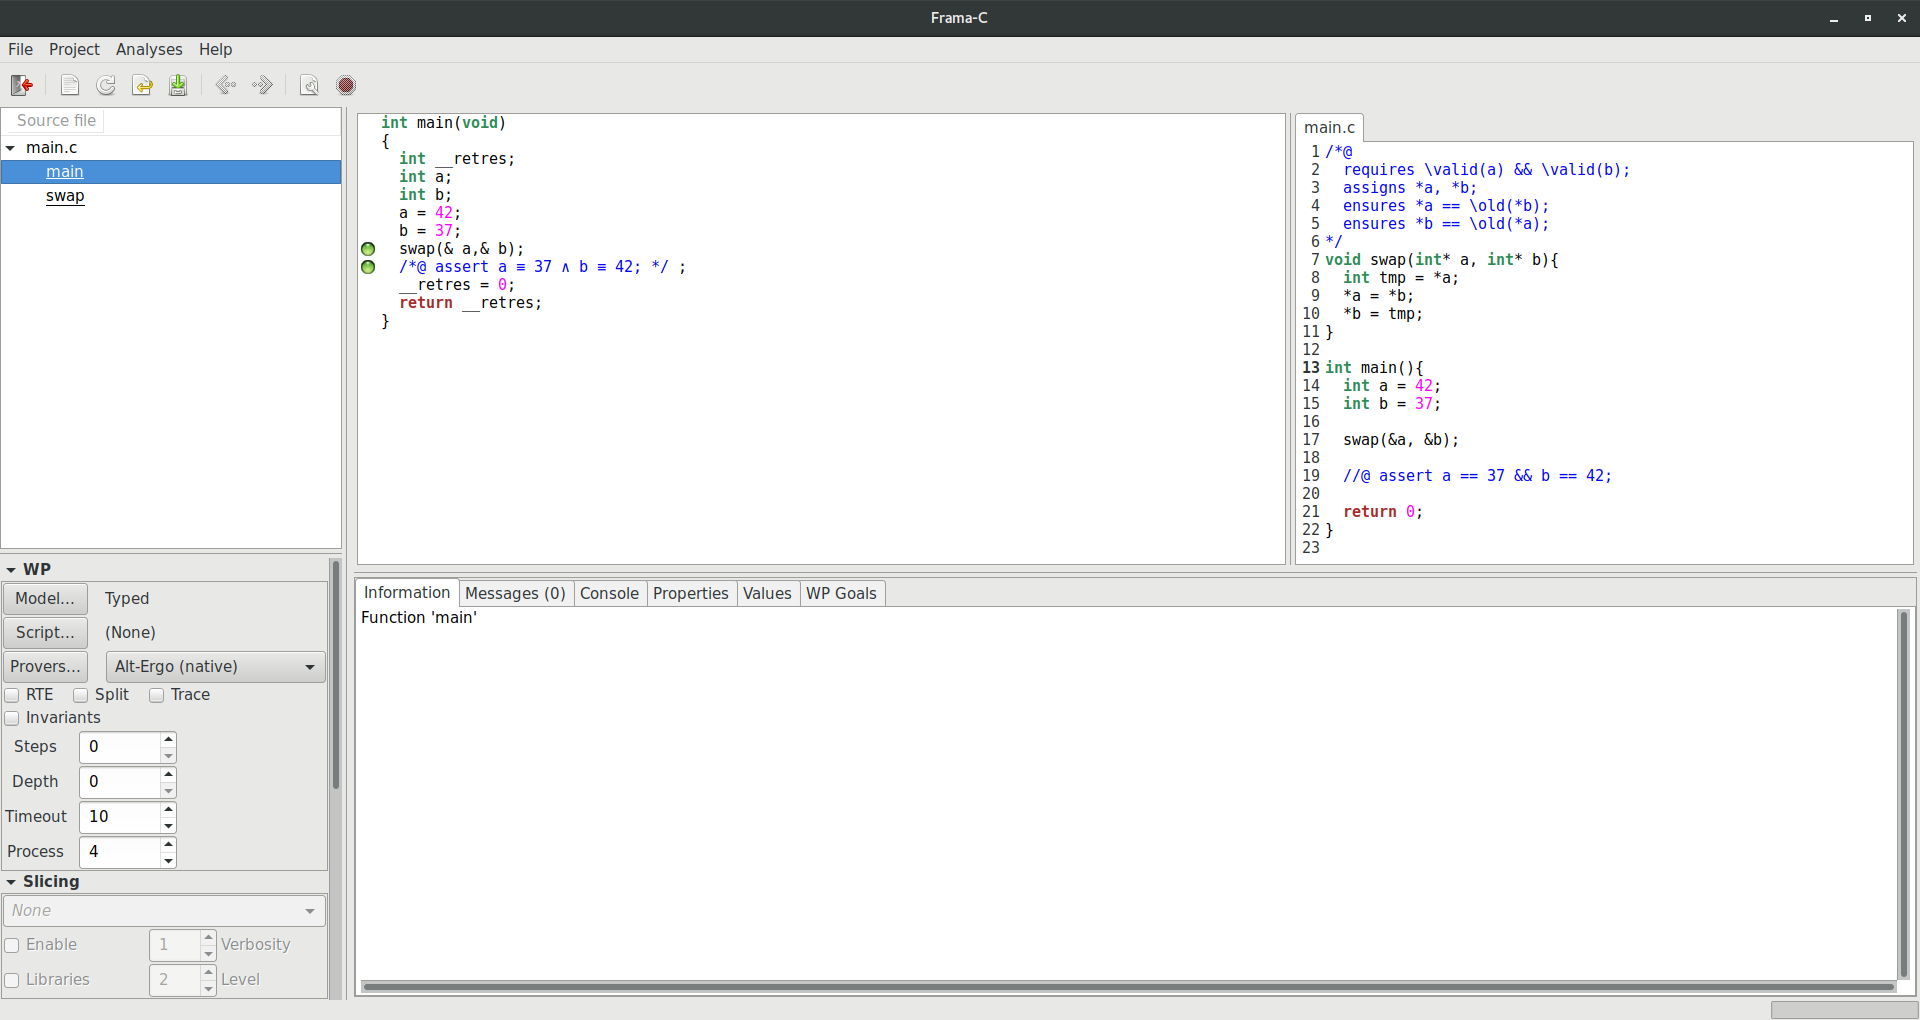
\includegraphics[scale=0.5]{1-2-verif_install-1.png}
\caption{Verify installation 1}
\label{fig:install-1}
\end{figure}

Clicking \texttt{main.c} in the left side panel to select it, we can see
its content (slightly) modified, and some green bullets on different
lines as illustrated by Figure~\ref{fig:install-2}.

\begin{figure}[htbp]
\centering
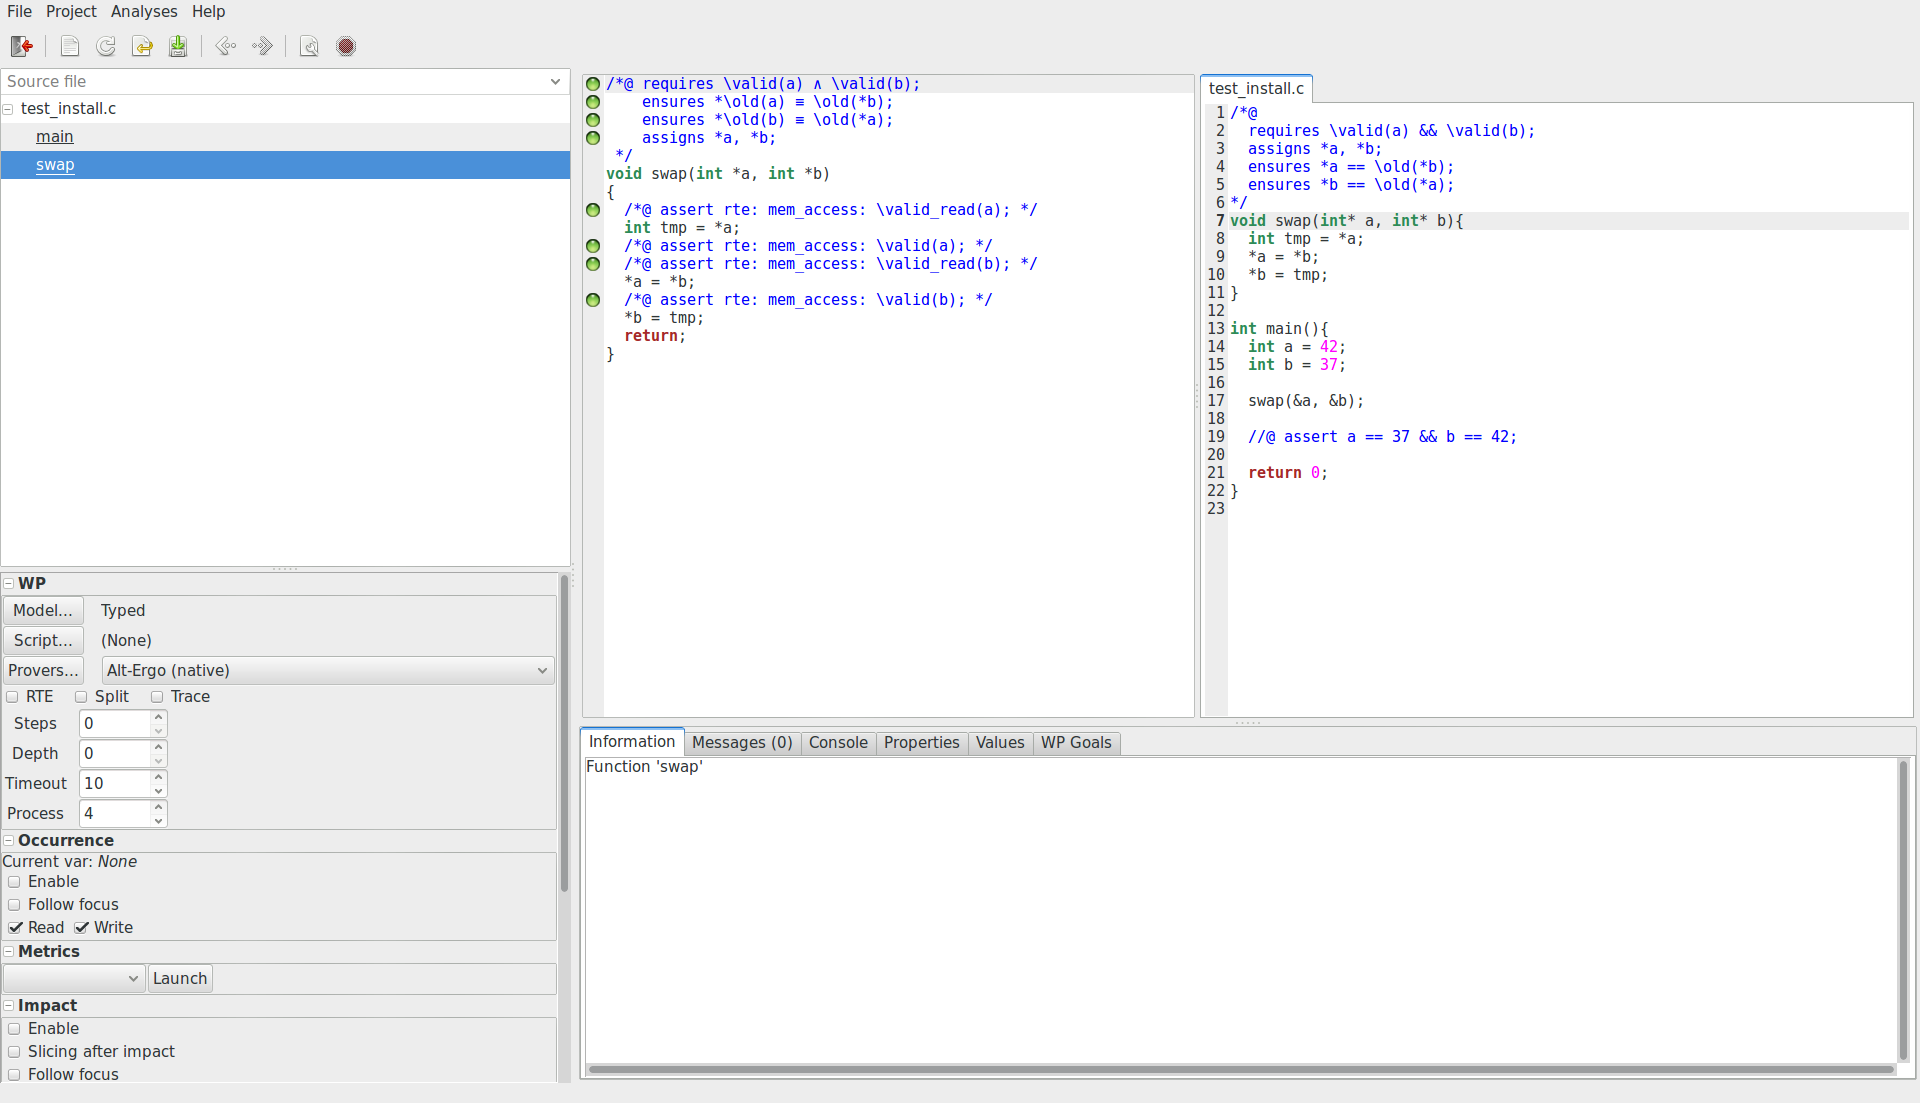
\includegraphics[scale=0.5]{1-2-verif_install-2.png}
\caption{Verify installation 2}
\label{fig:install-2}
\end{figure}

\begin{zdsalertblock}{Warning}
  The graphical user interface of Frama-C does not allow source code edition
\end{zdsalertblock}

\begin{zdsblock}{Information}
  For color blinds, it is possible to start Frama-C with another theme where
  color bullets are replaced:
  \begin{footnotesize}\begin{Shaded}
      \begin{Highlighting}[]
        \KeywordTok{$} \KeywordTok{frama-c-gui} \KeywordTok{-gui-theme} \KeywordTok{colorblind} \KeywordTok{file.c}
      \end{Highlighting}
  \end{Shaded}\end{footnotesize}
\end{zdsblock}

\subsection{(Bonus) Some more provers}\label{bonus-some-more-provers}

This part is optional, nothing in this section should be particularly
useful \emph{in the tutorial}. However, when we start to be interested
in proving more complex programs, it is often possible to reach the
limits of Alt-Ergo, which is basically available, and we would thus need
some other provers.

\subsubsection{Coq}\label{coq}

Coq, which is developed by Inria, is a proof assistant. Basically, we
write the proofs ourselves in a dedicated language and the platform
verify (using typing) that the proof is actually a valid proof.

Why would we need such a tool? Sometimes, the properties we want to
prove can be too complex to be solved automatically by SMT solvers,
typically when they requires careful inductive reasoning with precise
choices at each step. In this situation, WP allows us to generate proof
goals translated in Coq language, and to write the proof ourselves.

To learn Coq, we would recommend
\href{http://www.cis.upenn.edu/~bcpierce/sf/current/index.html}{this
tutorial}.

\begin{zdsblock}{Information}
  If Frama-C has been installed using the package manager of a Linux
  distribution, Coq could be automatically installed.
\end{zdsblock}

If one needs more information about Coq and its installation, this page
can help: \href{https://coq.inria.fr/}{The Coq Proof Assistant}.

When we want to use Coq for a proof with Frama-C, we have to select it
using the left side panel, in the WP part (see Figure~\ref{fig:select_coq}).

\begin{figure}[htbp]
\centering
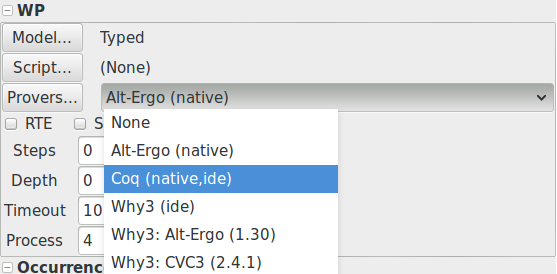
\includegraphics[scale=0.5]{1-2-select-coq.png}
\caption{Select the Coq proof assistant}
\label{fig:select_coq}
\end{figure}

\begin{zdsblock}{Information}
  The author does not know if it works under Windows.
\end{zdsblock}

\subsubsection{Why3}\label{why3}

\begin{zdsalertblock}{Warning}
  To the author's knowledge, it is not possible (or, at least, not easy
  at all) to install Why3 under Windows. The author cannot be charged for
  injuries that could result of such an operation.
\end{zdsalertblock}
  
Why3 is deductive proof platform developed by the LRI in Orsay. It
provides a programming language and a specification language, as well as
a module that allows to interact with a wide variety of automatic and
interactive provers. This point is the one that interest us here. WP can
translate its proof goals to the Why3 language and then use Why3 to
interact with solvers.

The \href{http://why3.lri.fr/}{Why3 website} provides all information
about it. If Opam is installed, Why3 is available using it, else, there
is an another installation procedure.

On this website, we can find the list of
\href{http://why3.lri.fr/\#provers}{supported provers}. We recommend to
install \href{https://github.com/Z3Prover/z3/wiki}{Z3} which is
developed by Microsoft Research, and
\href{http://cvc4.cs.nyu.edu/web/}{CVC4} which is developed by many
research teams (New York University, University of Iowa, Google, CEA
List). Those two provers are very efficient and somewhat complementary.

To use these provers, the procedure is explained in the Coq part that
describes the selection of a prover for the proof. Notice that it could
be necessary to ask the detection of freshly installed provers using the
``Provers'' button and then ``Detect Provers'' in the window that should
pop.

Our tools are now installed and ready to be used.

The goal of this part, apart of the installation of our tools was to put
in relief two main ideas:

\begin{itemize}
\tightlist
\item
  program proof is a way to ensure that our programs only have correct
  behaviors, described by our specification,
\item
  it is still our work to ensure that this specification is correct.
\end{itemize}

\chapter{Function contract}\label{function-contract}

It is time to enter the heart of the matter. Rather than starting with
basic notions of the C language, as we would do for a tutorial about C,
we will start with functions. First because it is necessary to be able
to write functions before starting this tutorial (to be able to prove
that a code is correct, being able to write it correct is required), and
then because it will allow us to directly prove some programs.

After this part about functions, we will on the opposite focus on simple
notions like assignments or conditonal structures, to understand how our
tool really works.

In order to be able to prove that a code is valid, we first need to
specify what we expect of it. Building the proof of our program consists
in ensuring that the code we wrote corresponds to the specification that
describes its job. As we previously said, Frama-C provides the ACSL
language to let the developer write contracts about each function (but
that is not its only purpose, as we will see later).

\section{Contract definition}\label{contract-definition}

The goal of a function contract is to state the conditions under which
the function will execute. That is to say, what the function expect from
the caller to ensure that it will correctly behave: the precondition,
the notion of ``correctly behave'' being itself defined in the contract
by the postcondition.

These properties are expressed with ACSL, the syntax is relatively
simple if one have already developed in C language since it shares most
of the syntax of boolean expressions in C. However, it also provides:

\begin{itemize}
\tightlist
\item
  some logic constructs and connectors that do not exists in C, to ease
  the writing of specifications,
\item
  built-in predicates to express properties that are useful about C
  programs (for example: a valid pointer),
\item
  as well as some primitive types for the logic that are more general
  than primitive C types (for example: mathematical integer).
\end{itemize}

We will introduce along this tutorial a large part of the notations
available in ACSL.

ACSL specifications are introduced in our source code using annotations.
Syntactically, a function contract is integrated in the source code with
this syntax:

\begin{footnotesize}\begin{Shaded}
\begin{Highlighting}[]
\CommentTok{/*@}
\CommentTok{  //contract}
\CommentTok{*/}
\DataTypeTok{void} \NormalTok{foo(}\DataTypeTok{int} \NormalTok{bar)\{}

\NormalTok{\}}
\end{Highlighting}
\end{Shaded}\end{footnotesize}

Notice the \texttt{@} at the beginning of the comment block, this
indicates to Frama-C that what follows are annotations and not a comment
block that it should simply ignore.

Now, let us have a look to the way we express contracts, starting with
postconditions, since it is what we want our function to do (we will
later see how to express precondition).

\subsection{Postcondition}\label{postcondition}

The postcondition of a function is introduced with the clause
\texttt{ensures}. We will illustrate its use with the following function
that returns the absolute value of an input. One of its postconditions
is that the result (which is denoted with the keywork
\texttt{\textbackslash{}result}) is greater or equal to 0.

\begin{footnotesize}\begin{Shaded}
\begin{Highlighting}[]
\CommentTok{/*@}
\CommentTok{  ensures \textbackslash{}result >= 0;}
\CommentTok{*/}
\DataTypeTok{int} \NormalTok{abs(}\DataTypeTok{int} \NormalTok{val)\{}
  \KeywordTok{if}\NormalTok{(val < }\DecValTok{0}\NormalTok{) }\KeywordTok{return} \NormalTok{-val;}
  \KeywordTok{return} \NormalTok{val;}
\NormalTok{\}}
\end{Highlighting}
\end{Shaded}\end{footnotesize}

(Notice the \texttt{;} at the end of the line, exactly as we do in C).

But that it is not the only property to verify, we also need to specify
the general behavior of a function returning the absolute value. That
is: if the value is positive or 0, the function returns the same value,
else it returns the opposite of the value.

We can specify multiple postconditions, first by combining them with a
\texttt{\&\&} as we do in C, or by introducing a new \texttt{ensures}
clause, as we illustrate here:

\begin{footnotesize}\begin{Shaded}
\begin{Highlighting}[]
\CommentTok{/*@}
\CommentTok{  ensures \textbackslash{}result >= 0;}
\CommentTok{  ensures (val >= 0 ==> \textbackslash{}result == val ) && }
\CommentTok{          (val <  0 ==> \textbackslash{}result == -val);}
\CommentTok{*/}
\DataTypeTok{int} \NormalTok{abs(}\DataTypeTok{int} \NormalTok{val)\{}
  \KeywordTok{if}\NormalTok{(val < }\DecValTok{0}\NormalTok{) }\KeywordTok{return} \NormalTok{-val;}
  \KeywordTok{return} \NormalTok{val;}
\NormalTok{\}}
\end{Highlighting}
\end{Shaded}\end{footnotesize}

This specification is the opportunity to present a very useful logic
connector provided by ACSL and that does not exist in C: the implication
\(A \Rightarrow B\), that is written \texttt{A\ ==\textgreater{}\ B} in
ACSL. The truth table of the implication is the following:

\begin{longtable}[]{@{}lll@{}}
\toprule
\(A\) & \(B\) & \(A \Rightarrow B\)\tabularnewline
\midrule
\endhead
\(F\) & \(F\) & \(T\)\tabularnewline
\(F\) & \(T\) & \(T\)\tabularnewline
\(T\) & \(F\) & \(F\)\tabularnewline
\(T\) & \(T\) & \(T\)\tabularnewline
\bottomrule
\end{longtable}

That means that an implication \(A \Rightarrow B\) is true in two cases:
either \(A\) is false (and in this case, we do not check the value of
\(B\)), or \(A\) is true and then \(B\) must also be true. The idea
finally being ``I want to know if when \(A\) is true, \(B\) also is. If
\(A\) is false, I don't care, I consider that the complete formula is
true''.

Another available connector is the equivalence \(A \Leftrightarrow B\)
(written \texttt{A\ \textless{}==\textgreater{}\ B} in ACSL), and it is
stronger. It is conjunction of the implication in both ways
\((A \Rightarrow B) \wedge (B \Rightarrow A)\). This formula is true in
only two cases: \(A\) and \(B\) are both ture, or false (it can be seen
as the negation of the exclusive or).

\begin{zdsblock}{Information}
Let's give a quick reminder about all
truth tables of usual logic connectors in first order logic
(\(\neg\) = \texttt{!}, \(\wedge\) = \texttt{\&\&}, \(\vee\) =
\texttt{\textbar{}\textbar{}}) :
\begin{longtable}[]{@{}ccccccc@{}}
\(A\) & \(B\) & \(\neg A\) & \(A \wedge B\) & \(A \vee B\) & \(A \Rightarrow B\) & \(A \Leftrightarrow B\)\tabularnewline
\midrule
\endhead
\(F\) & \(F\) & \(V\) & \(F\) & \(F\) & \(V\) &\(V\)\tabularnewline
\(F\) & \(V\) & \(V\) & \(F\) & \(V\) & \(V\) &\(F\)\tabularnewline
\(V\) & \(F\) & \(F\) & \(F\) & \(V\) & \(F\) &\(F\)\tabularnewline
\(V\) & \(V\) & \(F\) & \(V\) & \(V\) & \(V\) &\(T\)\tabularnewline
\bottomrule
\end{longtable}
\end{zdsblock}

We can come back to our specification. As our files become longer and
contains a lot of specifications, if can be useful to name the
properties we want to verify. So, in ACSL, we can specify a name
(without spaces) followed by a \texttt{:}, before stating the property.
It is possible to put multiple levels of names to categorize our
properties. For example, we could write this:

\begin{footnotesize}\begin{Shaded}
\begin{Highlighting}[]
\CommentTok{/*@}
\CommentTok{  ensures positive_value: function_result: \textbackslash{}result >= 0;}
\CommentTok{  ensures (val >= 0 ==> \textbackslash{}result == val) && }
\CommentTok{          (val < 0 ==> \textbackslash{}result == -val);}
\CommentTok{*/}
\DataTypeTok{int} \NormalTok{abs(}\DataTypeTok{int} \NormalTok{val)\{}
  \KeywordTok{if}\NormalTok{(val < }\DecValTok{0}\NormalTok{) }\KeywordTok{return} \NormalTok{-val;}
  \KeywordTok{return} \NormalTok{val;}
\NormalTok{\}}
\end{Highlighting}
\end{Shaded}\end{footnotesize}

In most of this tutorial, we will not name the properties we want to
prove, since they will be generally quite simple and we will not have
too many of them, names would not give us much information.

We can copy and paste the function \texttt{abs} and its specification in
a file \texttt{abs.c} and use Frama-C to determine if the implementation
is correct against the specification. We can start the GUI of Frama-C
(it is also possible to use the command line interface of Frama-C but we
will not use it during this tutorial) by using this command line:

\begin{footnotesize}\begin{Shaded}
\begin{Highlighting}[]
\NormalTok{$ }\KeywordTok{frama-c-gui}
\end{Highlighting}
\end{Shaded}\end{footnotesize}

Or by opening it from the graphical environment.

It is then possible to click on the button ``Create a new session from
existing C files'', files to analyze can be selected by double-clicking
it, the OK button ending the selection. Then, adding other files will be
done by clicking Files \textgreater{} Source Files.

Notice that it is also possible to directly open file(s) from the
terminal command line passing them to Frama-C as parameter(s):

\begin{footnotesize}\begin{Shaded}
\begin{Highlighting}[]
\NormalTok{$ }\KeywordTok{frama-c-gui} \NormalTok{abs.c}
\end{Highlighting}
\end{Shaded}\end{footnotesize}

\begin{figure}[htbp]
\centering
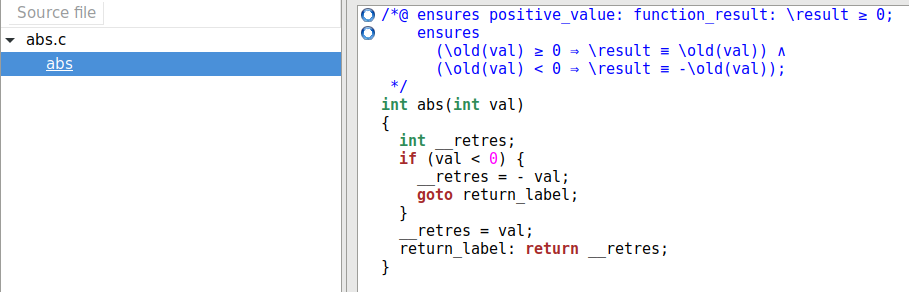
\includegraphics[scale=0.5]{2-1-1-abs-1.png}
\caption{The side panel gives the files and functions tree}
\label{fig:2-1-1-abs-1}
\end{figure}

The window of Frama-C opens and in the panel dedicated to files and
functions, we can select the function \texttt{abs}. At each
\texttt{ensures} line, we can see a blue circle, it indicates that no
verification has been attempted for these properties
(see Figure~\ref{fig:2-1-1-abs-1}).

We ask the verification of the code by right-clicking the name of the
function and ``Prove function annotations by WP''
(see Figure~\ref{fig:2-1-1-abs-2}).

\begin{figure}[htbp]
\centering
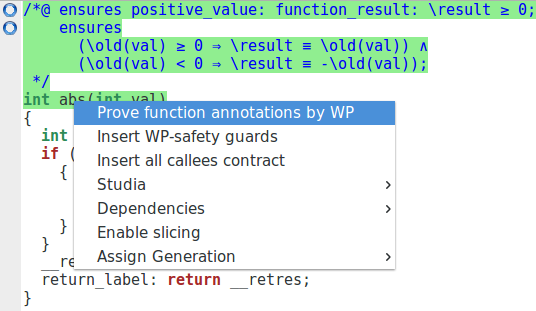
\includegraphics[scale=0.5]{2-1-1-abs-2.png}
\caption{Start the verification of \texttt{abs} with WP}
\label{fig:2-1-1-abs-2}
\end{figure}

We can see that blue circles become green bullets, indicating that the
specification is indeed ensured by the program. We can also prove
properties one by one by right-clicking on them and not on the name of
the function.

But is our code really bug free ? WP gives us a way to ensure that a
code respects a specification, but it does not check for runtime errors
(RTE). This is provided by another plugin that we will use here and that
is called RTE. Its goal is to add, in the program, some controls to
ensure that the program cannot create runtime errors (integer overflow,
invalid pointer dereferencing, 0 division, etc).

To active these controls, we check the box pointed by the screenshot (in
the WP panel). We can also ask Frama-C to add them in a function by
right-clicking on its name and then click ``Insert RTE guards''
(see Figure~\ref{fig:2-1-1-abs-3}).

\begin{figure}[htbp]
\centering
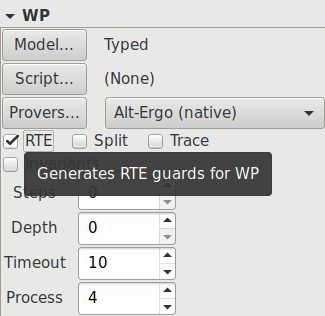
\includegraphics[scale=0.5]{2-1-1-abs-3.png}
\caption{Activate runtime error absence verification}
\label{fig:2-1-1-abs-3}
\end{figure}

Finally, we execute the verification again (we can also click on the
``Reparse'' button of the toolbar, it will deletes existing proofs).

We can then see that WP fails to prove the absence of arithmetic
underflow for the computation of \texttt{-val}. And, indeed, on our
architectures, \texttt{-INT\_MIN} (\(-2^{31}\)) \textgreater{}
\texttt{INT\_MAX} (\(2^{31}-1\)) (see Figure~\ref{fig:2-1-1-abs-4}).

\begin{figure}[htbp]
\centering
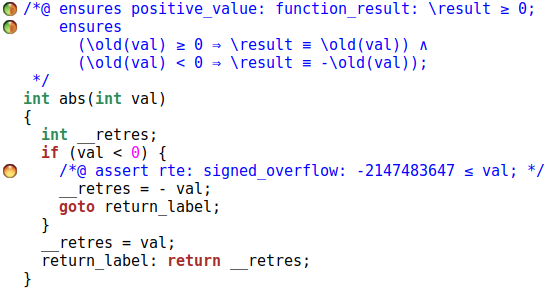
\includegraphics[scale=0.5]{2-1-1-abs-4.png}
\caption{Incomplete proof of \texttt{abs}}
\label{fig:2-1-1-abs-4}
\end{figure}

\begin{zdsblock}{Information}
We can notice that the underflow risk
is real for us, since our computers (for which the
configuration is detected by Frama-C) use the 
\href{https://en.wikipedia.org/wiki/Two\%27s_complement}{Two's
complement} implementation of integers, which do not defined
the behavior of under and overflows.
\end{zdsblock}

Here, we can see another type of ACSL annotation. By the line
\texttt{//@\ assert\ property\ ;}, we can ask the verification of
property at a particular program point. Here, RTE inserted for us, since
we have to verify that \texttt{-val} does not produce an underflow, but
we can also add such an assertion manually in the source code.

In this screenshot, we can see two new colors for our bullets:
green+brown and orange.

The green+brown color indicates that the proof has been produced but it
can depend on some properties that have not been verified.

If the proof has not been entirely redone after adding the runtime error
checks, these bullets must still be green. Indeed, the corresponding
proofs have been realized without the knowledge of the property in the
assertion, so they cannot rely on this unproved property.

When WP transmits a proof obligation to an automatic prover, it
basically transmits two types of properties : \(G\), the goal, the
property that we want to prove, and \(A_1\) \ldots{} \(A_n\), the
different assumptions we can have about the state of the memory at the
program point where we want to verify \(G\). However, it does not
receive (in return) the properties that have been used by the prover to
validate \(G\). So, if \(A_3\) is an assumption, and if WP did not
succeed in getting a proof of \(A_3\), it indicates that \(G\) is true,
but only if we succeed in proving \(A_3\).

The orange color indicates that no prover could determine if the
property is verified. There are two possibles reasons:

\begin{itemize}
\tightlist
\item
  the prover did not have enough information,
\item
  the prover did not have enough time to compute the proof and
  encountered a timeout (which can be configured in the WP panel).
\end{itemize}

In the bottom panel, we can select the ``WP Goals'' tab
(see Figure~\ref{fig:2-1-1-abs-5}), it shows the
list of proof obligations, and for each prover the result is symbolized
by a logo that indicates if the proof has been tried and if it
succeeded, failed or encountered a timeout (here we can see a try with
Z3 where we had a timeout on the proof of absence of RTE).

\begin{figure}[htbp]
\centering
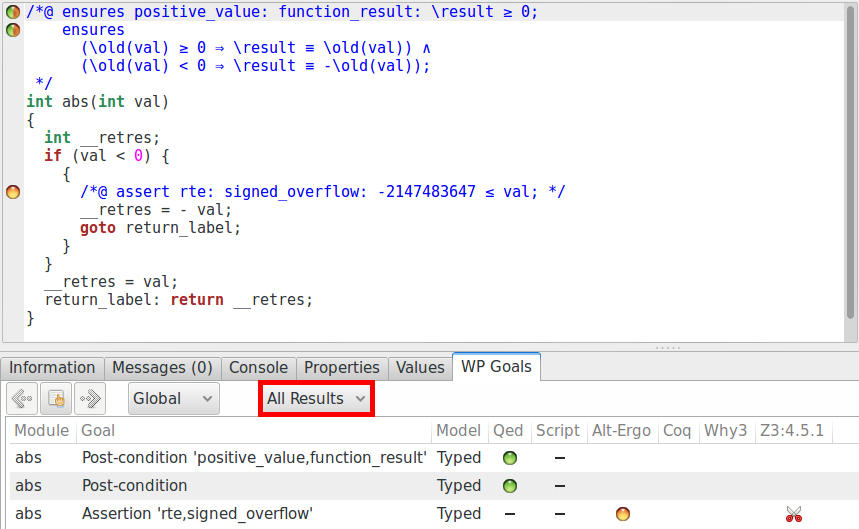
\includegraphics[scale=0.5]{2-1-1-abs-5.png}
\caption{Proof obligations panel of WP for \texttt{abs}}
\label{fig:2-1-1-abs-5}
\end{figure}

In the first column, we have the name of the function the proof
obligation belongs to. The second column indicates the name of proof
obligation. For example here, our postcondition is named
``Post-condition `positive\_value,function\_result'\,'', we can notice
that if we select a property in this list, it is also highlighted in the
source code. Unnamed properties are automatically named by WP with the
kind of wanted property. In the third column, we see the memory model
that is used for the proof, we will not talk about it in this tutorial.
Finally, the last columns represent the different provers available
through WP.

In these provers, the first element is Qed. It is not really a prover.
In fact, if we double-click on the property ``absence of underflow''
(highlight in blue in the last screenshot), we can see corresponding
proof obligation (see Figure~\ref{fig:2-1-1-abs-6}).

\begin{figure}[htbp]
\centering
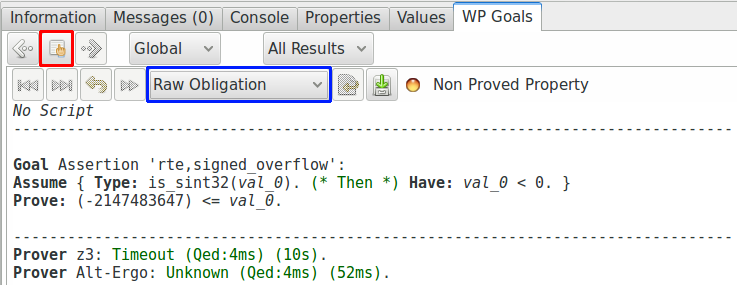
\includegraphics[scale=0.5]{2-1-1-abs-6.png}
\caption{Proof obligation associated to the verification of absence of
  underflow in \texttt{abs}}
\label{fig:2-1-1-abs-6}
\end{figure}

This is the proof obligation generated by WP about our property and our
program, we do need to understand everything here, but we can get the
general idea. It contains (in the ``Assume'' part) the assumptions that
we have specified and those that have been deduced by WP from the
instructions of the program. It also contains (in the ``Prove'' part)
the property that we want to verify.

What does WP do using these properties ? In fact, it transforms them
into a logic formula and then asks to different provers if it is
possible to satisfy this formula (to find for each variable, a value
that can make the formula true), and it determines if the property can
be proved. But before sending the formula to provers, WP uses a module
called Qed, which is able to perform different simplifications about it.
Sometimes, as this is the case for the other properties about
\texttt{abs}, these simplifications are enough to determine that the
property is true, in such a case, WP do not need the help of the
automatic solvers.

When automatic solvers cannot ensure that our properties are verified,
it it sometimes hard to understand why. Indeed, provers are generally
not able to answer something other than ``yes'', ``no'' or ``unknown'',
they are not able to extract the reason of a ``no'' or an ``unknown''.
There exists tools that can explore a proof tree to extract this type of
information, currently Frama-C do not provide such a tool. Reading proof
obligations can sometimes be helpful, but it requires a bit of practice
to be efficient. Finally, one of the best way to understand the reason
why a proof fails is to try to do it interactively with Coq. However, it
requires to be quite comfortable with this language to not being lost
facing the proof obligations generated by WP, since these obligations
need to encode some elements of the C semantics that can make them quite
hard to read.

If we go back to our view of proof obligations (see the squared button
in the last screenshot), we can see that our hypotheses are not enough
to determine that the property ``absence of underflow'' is true (which
is indeed currently impossible), so we need to add some hypotheses to
guarantee that our function will well-behave: a call precondition.

\subsection{Preconditon}\label{preconditon}

Preconditions are introduced using \texttt{requires} clauses. As we
could do with \texttt{ensures} clauses, we can compose logic expressions
and specify multiple preconditions:

\begin{footnotesize}\begin{Shaded}
\begin{Highlighting}[]
\CommentTok{/*@}
\CommentTok{  requires 0 <= a < 100;}
\CommentTok{  requires b < a;}
\CommentTok{*/}
\DataTypeTok{void} \NormalTok{foo(}\DataTypeTok{int} \NormalTok{a, }\DataTypeTok{int} \NormalTok{b)\{}
  
\NormalTok{\}}
\end{Highlighting}
\end{Shaded}\end{footnotesize}

Preconditions are properties about the input (and eventually about
global variables) that we assume to be true when we analyze the
function. We will verify that they are indeed true only at program
points where the function is called.

In this small example, we can also notice a difference with C in the
writing of boolean expressions. If we want to specify that \texttt{a} is
between 0 and 100, we do not have to write
\texttt{0\ \textless{}=\ a\ \&\&\ a\ \textless{}\ 100}, we can directly
write \texttt{0\ \textless{}=\ a\ \textless{}\ 100} and Frama-C will
perform necessary translations.

If we come back to our example about the absolute value, to avoid the
arithmetic underflow, it is sufficient to state that \texttt{val} must
be strictly greater than \texttt{INT\_MIN} to guarantee that the
underflow will never happen. We then add it as a precondition of the
function (notice that it is also necessary to include the header where
\texttt{INT\_MIN} is defined):

\begin{footnotesize}\begin{Shaded}
\begin{Highlighting}[]
\ErrorTok{#include <limits.h>}

\CommentTok{/*@}
\CommentTok{  requires INT_MIN < val;}

\CommentTok{  ensures \textbackslash{}result >= 0;}
\CommentTok{  ensures (val >= 0 ==> \textbackslash{}result == val) && }
\CommentTok{          (val < 0 ==> \textbackslash{}result == -val);}
\CommentTok{*/}
\DataTypeTok{int} \NormalTok{abs(}\DataTypeTok{int} \NormalTok{val)\{}
  \KeywordTok{if}\NormalTok{(val < }\DecValTok{0}\NormalTok{) }\KeywordTok{return} \NormalTok{-val;}
  \KeywordTok{return} \NormalTok{val;}
\NormalTok{\}}
\end{Highlighting}
\end{Shaded}\end{footnotesize}

\begin{zdsalertblock}{Warning}
  Reminder: The Frama-C GUI does not allow code source modification.
\end{zdsalertblock}
  
\begin{zdsblock}{Information}
For Frama-C NEON and older, the
pre-processing of annotations is not activated by default. We
have to start Frama-C with the option \texttt{-pp-annot}:

  \begin{footnotesize}\begin{Shaded}
\begin{Highlighting}[]
\KeywordTok{$} \KeywordTok{frama-c-gui} \KeywordTok{-pp-annot} \KeywordTok{file.c}
      \end{Highlighting}
  \end{Shaded}\end{footnotesize}
\end{zdsblock}

Once we have modified the source code with our precondition, we click on
``Reparse'' and we can ask again to prove our program. This time,
everything is validated by WP, our implementation is proved
(see Figure~\ref{fig:2-1-2-abs-1}).

\begin{figure}[htbp]
\centering
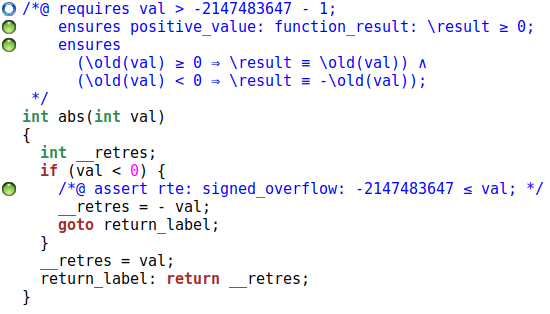
\includegraphics[scale=0.5]{2-1-2-abs-1.png}
\caption{Proof of \texttt{abs} performed}
\label{fig:2-1-2-abs-1}
\end{figure}

We can also verify that a function that would call \texttt{abs}
correctly respects the required precondition:

\begin{footnotesize}\begin{Shaded}
\begin{Highlighting}[]
\DataTypeTok{void} \NormalTok{foo(}\DataTypeTok{int} \NormalTok{a)\{}
   \DataTypeTok{int} \NormalTok{b = abs(}\DecValTok{42}\NormalTok{);}
   \DataTypeTok{int} \NormalTok{c = abs(-}\DecValTok{42}\NormalTok{);}
   \DataTypeTok{int} \NormalTok{d = abs(a);       }\CommentTok{// False : "a" can be INT_MIN}
   \DataTypeTok{int} \NormalTok{e = abs(INT_MIN); }\CommentTok{// False : the parameter must be strictly greater than INT_MIN}
\NormalTok{\}}
\end{Highlighting}
\end{Shaded}\end{footnotesize}

(The result is presented in Figure~\ref{fig:2-1-2-foo-1}).

\begin{figure}[htbp]
\centering
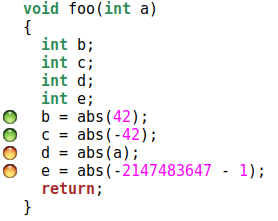
\includegraphics[scale=0.5]{2-1-2-foo-1.png}
\caption{Precondition checking when calling \texttt{abs}}
\label{fig:2-1-2-foo-1}
\end{figure}

We can modify this example by revering the last two instructions. If we
do this, we can see that the call \texttt{abs(a)} is validated by WP if
it is placed after the call \texttt{abs(INT\_MIN)}! Why?

We must keep in mind that the idea of the deductive proof is to ensure
that if preconditions are verified, and if our computation terminates,
then the post-conditon is verified.

If we give a function that surely breaks the precondition, we can deduce
that the postconditon is false. Knowing this, we can prove absolutely
everything because this ``false'' becomes an assumption of every call
that follows. Knowing false, we can prove everything, because if we have
a proof of false, then false is true, as well as true is true. So
everything is true.

Taking our modified program, we can convince ourselves of this fact by
looking at proof obligations generated by WP for the bad call and the
subsequent call that becomes verified (Figures~\ref{fig:2-1-2-foo-2}
and~\ref{fig:2-1-2-foo-3}).

\begin{figure}[htbp]
\centering
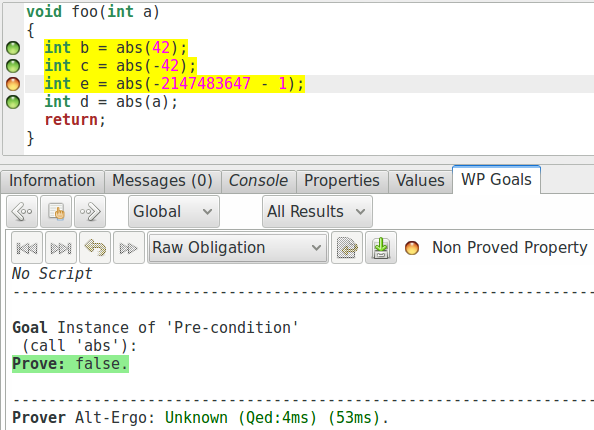
\includegraphics[scale=0.5]{2-1-2-foo-2.png}
\caption{Generated proof obligation for the bad call}
\label{fig:2-1-2-foo-2}
\end{figure}

\begin{figure}[htbp]
\centering
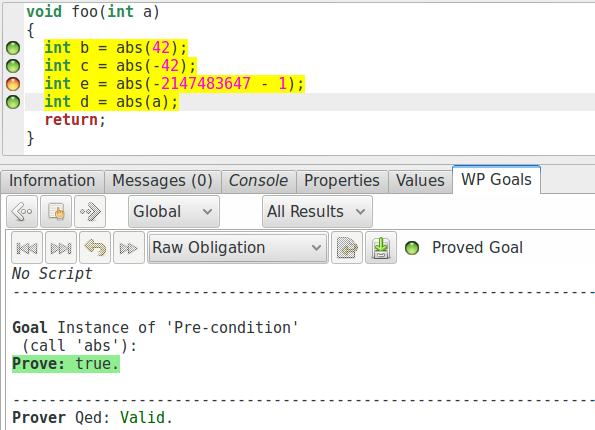
\includegraphics[scale=0.5]{2-1-2-foo-3.png}
\caption{Generated proof obligation for the call that follows}
\label{fig:2-1-2-foo-3}
\end{figure}

We can notice that for function calls, the GUI highlights the execution
path that leads to the call for which we want to verify the preconditon.
Then, if we have a closer look to the call \texttt{abs(INT\_MIN)}, we
can notice that, simplifying, Qed deduced that we try to prove
``False''. Consequently, the next call \texttt{abs(a)} receives in its
assumptions the property ``False''. This is why Qed can immediately
deduce ``True''.

The second part of the question is then: why our first version of the
calling function (\texttt{abs(a)} and then \texttt{abs(INT\_MIN)}) did
not have the same behavior, indicating a proof failure on the second
call? The answer is simply that the call \texttt{abs(a)} can, or not,
produce an error, whereas \texttt{abs(INT\_MIN)} necessarily leads to an
error. So, while \texttt{abs(INT\_MIN)} necessarily gives us the
knowledge of ``false'', the call \texttt{abs(a)} does not, since it can
succeed.

Produce a correct specification is then crucial. Typically, by stating
false precondition, we can have the possibility to create a proof of
false:

\begin{footnotesize}\begin{Shaded}
\begin{Highlighting}[]
\CommentTok{/*@}
\CommentTok{  requires a < 0 && a > 0;}
\CommentTok{  ensures  \textbackslash{}false;}
\CommentTok{*/}
\DataTypeTok{void} \NormalTok{foo(}\DataTypeTok{int} \NormalTok{a)\{}

\NormalTok{\}}
\end{Highlighting}
\end{Shaded}\end{footnotesize}

If we ask WP to prove this function, it will accept it without a problem
since the assumption we give in precondition is necessarily false.
However, we will not be able to give an input that respects the
precondition so we will be able to detect this problem by carefully
reading what we have specified.

Some notions we will see in this tutorial can expose us to the
possibility to introduce subtle incoherence. So, we must always be
careful specifying a program.

\subsubsection{Finding the right
preconditions}\label{finding-the-right-preconditions}

Finding the right preconditions for a function is sometimes hard. The
most important idea is to determine these preconditions without taking
in account the content of the function (at least, in a first step), in
order to avoid building a specification that would contain the same bugs
currently existing in the source code, for example taking in account an
erroneous conditional structure. In fact, it is generally a good
practice to work with someone else. One specifies the function and the
other implements it (even if they previously agreed on a common textual
specification).

Once these precondition has been stated, then we work on the
specifications that are due to the constraints of our language and our
hardware. For example, the absolute value do not really have a
precondition, this is our hardware that adds the condition we have given
in precondition due to the two's complement on which it relies.

\subsection{Some elements about the use of WP and
Frama-C}\label{some-elements-about-the-use-of-wp-and-frama-c}

In the two preceding sections, we have seen a lot of notions about the
use of the GUI to start proofs. In fact, we can ask WP to immediately
prove everything at Frama-C's startup with the option \texttt{-wp}:

\begin{footnotesize}\begin{Shaded}
\begin{Highlighting}[]
\NormalTok{$ }\KeywordTok{frama-c-gui} \NormalTok{file.c -wp}
\end{Highlighting}
\end{Shaded}\end{footnotesize}

Which will collect all properties to be proved inside \texttt{file.c},
generate all proof obligations and try to discharge them.

About runtime-errors, it is generally advised to first verify the
program without generating RTE assertions, and then to generate them to
terminate the verification with WP. It allows WP to ``focus'' on the
functional properties in a first step without having in its knowledge
base purely technical properties, that are generally not useful for the
proof of functional properties. Again, it is possible to directly
produce this behavior using the command line:

\begin{footnotesize}\begin{Shaded}
\begin{Highlighting}[]
\NormalTok{$ }\KeywordTok{frama-c-gui} \NormalTok{file.c -wp -then -rte -wp}
\end{Highlighting}
\end{Shaded}\end{footnotesize}

``Start Frama-C with WP, then create assertions to verify the absence of
RTE and start WP again''.

\section{Well specified function}\label{well-specified-function}

\subsection{Correctly write what we
expect}\label{correctly-write-what-we-expect}

This is certainly the hardest part of our work. Programming is already
an effort that consists in writing algorithms that correctly respond to
our need. Specifying request the same kind of work, except that we do
not try to express \emph{how} we respond to the need but \emph{what} is
exactly our need. To prove that our code implements what we need, we
must be able to describe exactly what we need.

From now, we will use an other example, the \texttt{max} function:

\begin{footnotesize}\begin{Shaded}
\begin{Highlighting}[]
\DataTypeTok{int} \NormalTok{max(}\DataTypeTok{int} \NormalTok{a, }\DataTypeTok{int} \NormalTok{b)\{}
  \KeywordTok{return} \NormalTok{(a > b) ? a : b;}
\NormalTok{\}}
\end{Highlighting}
\end{Shaded}\end{footnotesize}

The reader could write and prove their own specification. We will start
using this one:

\begin{footnotesize}\begin{Shaded}
\begin{Highlighting}[]
\CommentTok{/*@}
\CommentTok{  ensures \textbackslash{}result >= a && \textbackslash{}result >= b;}
\CommentTok{*/}
\DataTypeTok{int} \NormalTok{max(}\DataTypeTok{int} \NormalTok{a, }\DataTypeTok{int} \NormalTok{b)\{}
  \KeywordTok{return} \NormalTok{(a > b) ? a : b;}
\NormalTok{\}}
\end{Highlighting}
\end{Shaded}\end{footnotesize}

If we ask WP to prove this code, it will succeed without any problem.
However, is our specification really correct? We can try to prove this
calling code:

\begin{footnotesize}\begin{Shaded}
\begin{Highlighting}[]
\DataTypeTok{void} \NormalTok{foo()\{}
  \DataTypeTok{int} \NormalTok{a = }\DecValTok{42}\NormalTok{;}
  \DataTypeTok{int} \NormalTok{b = }\DecValTok{37}\NormalTok{;}
  \DataTypeTok{int} \NormalTok{c = max(a,b);}

  \CommentTok{//@assert c == 42;}
\NormalTok{\}}
\end{Highlighting}
\end{Shaded}\end{footnotesize}

There, it will fail. In fact, we can go further by modifying the body of
the \texttt{max} function and notice that the following code is also
correct with respect to the specification:

\begin{footnotesize}\begin{Shaded}
\begin{Highlighting}[]
\ErrorTok{#include <limits.h>}

\CommentTok{/*@}
\CommentTok{  ensures \textbackslash{}result >= a && \textbackslash{}result >= b;}
\CommentTok{*/}
\DataTypeTok{int} \NormalTok{max(}\DataTypeTok{int} \NormalTok{a, }\DataTypeTok{int} \NormalTok{b)\{}
  \KeywordTok{return} \NormalTok{INT_MAX;}
\NormalTok{\}}
\end{Highlighting}
\end{Shaded}\end{footnotesize}

Our specification is too permissive. We have to be more precise. We do
not only expect the result to be greater or equal to both parameters,
but also that the result is one of them:

\begin{footnotesize}\begin{Shaded}
\begin{Highlighting}[]
\CommentTok{/*@}
\CommentTok{  ensures \textbackslash{}result >= a && \textbackslash{}result >= b;}
\CommentTok{  ensures \textbackslash{}result == a || \textbackslash{}result == b;}
\CommentTok{*/}
\DataTypeTok{int} \NormalTok{max(}\DataTypeTok{int} \NormalTok{a, }\DataTypeTok{int} \NormalTok{b)\{}
  \KeywordTok{return} \NormalTok{(a > b) ? a : b;}
\NormalTok{\}}
\end{Highlighting}
\end{Shaded}\end{footnotesize}

\subsection{Pointers}\label{pointers}

If there is one notion that we permanently have to confront with in C
language, this is definitely the notion of pointer. Pointers are quite
hard to manipulate correctly, and they still are the main source of
critical bugs in programs, so they benefit of a preferential treatment
in ACSL.

We can illustrate with a swap function for C integers:

\begin{footnotesize}\begin{Shaded}
\begin{Highlighting}[]
\CommentTok{/*@}
\CommentTok{  ensures *a == \textbackslash{}old(*b) && *b == \textbackslash{}old(*a);}
\CommentTok{*/}
\DataTypeTok{void} \NormalTok{swap(}\DataTypeTok{int}\NormalTok{* a, }\DataTypeTok{int}\NormalTok{* b)\{}
  \DataTypeTok{int} \NormalTok{tmp = *a;}
  \NormalTok{*a = *b;}
  \NormalTok{*b = tmp;}
\NormalTok{\}}
\end{Highlighting}
\end{Shaded}\end{footnotesize}

\subsubsection{History of values in
memory}\label{history-of-values-in-memory}

Here, we introduce a first built-in logic function of ACSL:
\texttt{old}, that allows us to get the old value of a given element.
So, our specification defines that the function must ensure that after
the call, the value of \texttt{*a} is the old (that is to say, before
the call) value of \texttt{*b} and conversely.

The \texttt{\textbackslash{}old} function can only be used in the
post-condition of a function. If we need this type of information
somewhere else, we will use \texttt{at} that allows us to express that
we want the value of a variable at a particular program point. This
function receives two parameters. The first one is the variable (or
memory location) for which we want to get its value and the second one
is the program point (as a C label) that we want to consider.

For example, we could write:

\begin{footnotesize}\begin{Shaded}
\begin{Highlighting}[]
  \DataTypeTok{int} \NormalTok{a = }\DecValTok{42}\NormalTok{;}
 \NormalTok{Label_a:}
  \NormalTok{a = }\DecValTok{45}\NormalTok{;}

  \CommentTok{//@assert a == 45 && \textbackslash{}at(a, Label_a) == 42;}
\end{Highlighting}
\end{Shaded}\end{footnotesize}

Of course, we can use any C label in our code, but we also have 6
built-in labels defined by ACSL that can be used, however WP does not
support all of them currently:

\begin{itemize}
\tightlist
\item
  \texttt{Pre}/\texttt{Old} : value before function call,
\item
  \texttt{Post} : value after function call,
\item
  \texttt{LoopEntry} : value at loop entry (not supported yet),
\item
  \texttt{LoopCurrent} : value at the beginning of the current step of
  the loop (not supported yet),
\item
  \texttt{Here} : value at the current program point.
\end{itemize}

\begin{zdsblock}{Information}
  The behavior of \texttt{Here} is in fact the default behavior when we
  consider a variable. Its use with \texttt{at} with generally let us
  ensure that what we write is not ambigous, and is more readable, when
  we express properties about values at different program points in the
  same expression.
\end{zdsblock}

Whereas \texttt{\textbackslash{}old} can only be used in function
post-conditions, \texttt{\textbackslash{}at} can be used anywhere.
However, we cannot use any program point with respect to the type
annotation we are writing. \texttt{Old} and \texttt{Post} are only
available in function post-conditions, \texttt{Pre} and \texttt{Here}
are available everywhere. \texttt{LoopEntry} and \texttt{LoopCurrent}
are only available in the context of loops (which we will detail later
in this tutorial).

At the moment, we will not need \texttt{\textbackslash{}at} but it can
often be useful, if not essential, when we want to make our
specification precise.

\subsubsection{Pointers validity}\label{pointers-validity}

If we try to prove that the swap function is correct (comprising RTE
verification), our post-condition is indeed verified but WP failed to
prove some possibilities of runtime-error, since we perform access to
some pointers that we did not indicate to be valid pointers in the
precondition of the function.

We can express that the dereferencing of a pointer is valid using the
\texttt{\textbackslash{}valid} predicate of ACSL which receives the
pointer in input:

\begin{footnotesize}\begin{Shaded}
\begin{Highlighting}[]
\CommentTok{/*@}
\CommentTok{  requires \textbackslash{}valid(a) && \textbackslash{}valid(b);}
\CommentTok{  ensures  *a == \textbackslash{}old(*b) && *b == \textbackslash{}old(*a);}
\CommentTok{*/}
\DataTypeTok{void} \NormalTok{swap(}\DataTypeTok{int}\NormalTok{* a, }\DataTypeTok{int}\NormalTok{* b)\{}
  \DataTypeTok{int} \NormalTok{tmp = *a;}
  \NormalTok{*a = *b;}
  \NormalTok{*b = tmp;}
\NormalTok{\}}
\end{Highlighting}
\end{Shaded}\end{footnotesize}

Once we have specified that the pointers we receive in input are valid,
dereferencing is assured to not produce undefined behaviors.

As we will see later in this tutorial, \texttt{\textbackslash{}valid}
can take more than one pointer in parameter. For example, we can give it
an expression such as: \texttt{valid(p\ +\ (s\ ..\ e))} which means
``for all \texttt{i} between included \texttt{s} and \texttt{e},
\texttt{p+i} is a valid pointer. This kind of expression will be
extremely useful when we will specify properties about arrays in
specifications.

If we have a closer look to the assertions that WP adds in the swap
function comprising RTE verification, we can notice that there exists
another version of the \texttt{\textbackslash{}valid} predicate, denoted
\texttt{\textbackslash{}valid\_read}. As opposed to \texttt{valid}, the
predicate \texttt{\textbackslash{}valid\_read} indicates that a pointer
can be dereferenced, but only to read the pointed memory. This subtlety
is due to the C language, where the downcast of a const pointer is easy
to write but is not necessarily legal.

Typically, in this code:

\begin{footnotesize}\begin{Shaded}
\begin{Highlighting}[]
\CommentTok{/*@ requires \textbackslash{}valid(p); */}
\DataTypeTok{int} \NormalTok{unref(}\DataTypeTok{int}\NormalTok{* p)\{}
  \KeywordTok{return} \NormalTok{*p;}
\NormalTok{\}}

\DataTypeTok{int} \DataTypeTok{const} \NormalTok{value = }\DecValTok{42}\NormalTok{;}

\DataTypeTok{int} \NormalTok{main()\{}
  \DataTypeTok{int} \NormalTok{i = unref(&value);}
\NormalTok{\}}
\end{Highlighting}
\end{Shaded}\end{footnotesize}

Dereferencing \texttt{p} is valid, however the precondition of
\texttt{unref} will not be verified by WP since dereferencing
\texttt{value} is only legal for a read-access. A write access will
result in an undefined behavior. In such a case, we can specify that the
pointer \texttt{p} must be \texttt{\textbackslash{}valid\_read} and not
\texttt{\textbackslash{}valid}.

\subsubsection{Side effects}\label{side-effects}

Our \texttt{swap} function is provable with regard to the specification
and potential runtime errors, but is it however specified enough? We can
slightly modify our code to check this (we use \texttt{assert} to verify
some properties at some particular points):

\begin{footnotesize}\begin{Shaded}
\begin{Highlighting}[]
\DataTypeTok{int} \NormalTok{h = }\DecValTok{42}\NormalTok{; }\CommentTok{//we add a global variable}

\CommentTok{/*@}
\CommentTok{  requires \textbackslash{}valid(a) && \textbackslash{}valid(b);}
\CommentTok{  ensures  *a == \textbackslash{}old(*b) && *b == \textbackslash{}old(*a);}
\CommentTok{*/}
\DataTypeTok{void} \NormalTok{swap(}\DataTypeTok{int}\NormalTok{* a, }\DataTypeTok{int}\NormalTok{* b)\{}
  \DataTypeTok{int} \NormalTok{tmp = *a;}
  \NormalTok{*a = *b;}
  \NormalTok{*b = tmp;}
\NormalTok{\}}

\DataTypeTok{int} \NormalTok{main()\{}
  \DataTypeTok{int} \NormalTok{a = }\DecValTok{37}\NormalTok{;}
  \DataTypeTok{int} \NormalTok{b = }\DecValTok{91}\NormalTok{;}

  \CommentTok{//@ assert h == 42;}
  \NormalTok{swap(&a, &b);}
  \CommentTok{//@ assert h == 42;}
\NormalTok{\}}
\end{Highlighting}
\end{Shaded}\end{footnotesize}

The result is not exactly what we expect, as we can see in
Figure~\ref{fig:2-2-2-swap-1}.

\begin{figure}[htbp]
\centering
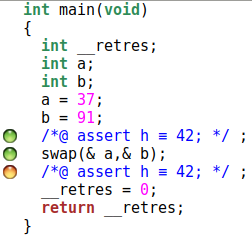
\includegraphics[scale=0.5]{2-2-2-swap-1.png}
\caption{Proof failure on the property of a global variable which is not
  modified by \texttt{swap}}
\label{fig:2-2-2-swap-1}
\end{figure}

Indeed, we did not specify the allowed side effects for our function. In
order to specify side effects, we use an \texttt{assign} clause which is
part of the postcondition of a function. It allows us to specify which
\textbf{non local} elements (we verify side effects) can be modified
during the execution of the function.

By default, WP considers that a function can modify everything in the
memory. So, we have to specify what can be modified by a function. For
example, our \texttt{swap} function will be specified like this:

\begin{footnotesize}\begin{Shaded}
\begin{Highlighting}[]
\CommentTok{/*@}
\CommentTok{  requires \textbackslash{}valid(a) && \textbackslash{}valid(b);}
\CommentTok{ }
\CommentTok{  assigns *a, *b;}

\CommentTok{  ensures  *a == \textbackslash{}old(*b) && *b == \textbackslash{}old(*a);}
\CommentTok{*/}
\DataTypeTok{void} \NormalTok{swap(}\DataTypeTok{int}\NormalTok{* a, }\DataTypeTok{int}\NormalTok{* b)\{}
  \DataTypeTok{int} \NormalTok{tmp = *a;}
  \NormalTok{*a = *b;}
  \NormalTok{*b = tmp;}
\NormalTok{\}}
\end{Highlighting}
\end{Shaded}\end{footnotesize}

If we ask WP to prove the function with this specification, it will be
validated (including with the variable added in the previous source
code).

Finally, we sometimes want to specify that a function is side effect
free. We specify this by giving \texttt{\textbackslash{}nothing} to
\texttt{assigns}:

\begin{footnotesize}\begin{Shaded}
\begin{Highlighting}[]
\CommentTok{/*@}
\CommentTok{  requires \textbackslash{}valid_read(a) && \textbackslash{}valid_read(b);}

\CommentTok{  assigns  \textbackslash{}nothing;}

\CommentTok{  ensures \textbackslash{}result == *a || \textbackslash{}result == *b;}
\CommentTok{  ensures \textbackslash{}result >= *a && \textbackslash{}result >= *b;}
\CommentTok{*/}
\DataTypeTok{int} \NormalTok{max_ptr(}\DataTypeTok{int}\NormalTok{* a, }\DataTypeTok{int}\NormalTok{* b)\{}
  \KeywordTok{return} \NormalTok{(*a > *b) ? *a : *b ;}
\NormalTok{\}}
\end{Highlighting}
\end{Shaded}\end{footnotesize}

The careful reader will now be able to take back the examples we
presented until now to integrate the right \texttt{assigns} clause.

\subsubsection{Memory location
separation}\label{memory-location-separation}

Pointers bring the risk of aliasing (multiple pointers can have access
to the same memory location). For some functions, it will not cause any
problem, for example when we give two identical pointers to the
\texttt{swap} function, the specification is still verified. However,
sometimes it is not that simple:

\begin{footnotesize}\begin{Shaded}
\begin{Highlighting}[]
\ErrorTok{#include <limits.h>}

\CommentTok{/*@}
\CommentTok{  requires \textbackslash{}valid(a) && \textbackslash{}valid_read(b);}
\CommentTok{  assigns  *a;}
\CommentTok{  ensures  *a == \textbackslash{}old(*a)+ *b;}
\CommentTok{  ensures  *b == \textbackslash{}old(*b);}
\CommentTok{*/}
\DataTypeTok{void} \NormalTok{incr_a_by_b(}\DataTypeTok{int}\NormalTok{* a, }\DataTypeTok{int} \DataTypeTok{const}\NormalTok{* b)\{}
  \NormalTok{*a += *b;}
\NormalTok{\}}
\end{Highlighting}
\end{Shaded}\end{footnotesize}

If we ask WP to prove this function, we get the result illustrated in
Figure~\ref{fig:2-2-2-incr_a_by_b-1}.

\begin{figure}[htbp]
\centering
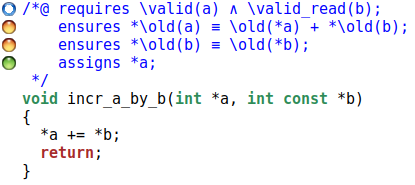
\includegraphics[scale=0.5]{2-2-2-incr_a_by_b-1.png}
\caption{Proof failure: potential aliasing}
\label{fig:2-2-2-incr_a_by_b-1}
\end{figure}

The reason is simply that we do not have any guarantee that the pointer
\texttt{a} is different of the pointer \texttt{b}. Now, if these
pointers are the same,

\begin{itemize}
\tightlist
\item
  the property \texttt{*a\ ==\ \textbackslash{}old(*a)\ +\ *b} in fact
  means \texttt{*a\ ==\ \textbackslash{}old(*a)\ +\ *a} which can only
  be true if the old value pointed by \texttt{a} was \(0\), and we do
  not have such a requirement,
\item
  the property \texttt{*b\ ==\ \textbackslash{}old(*b)} is not validated
  because we potentially modify this memory location.
\end{itemize}

\begin{zdsexampleblock}{Why is the \texttt{assign} clause validated ?}
  The reason is simply that \texttt{a} is indeed the only modified memory
  location. If \texttt{a\ !=\ b}, we only modify the location pointed by
  \texttt{a}, and if \texttt{a\ ==\ b}, \textbar{} that is still the case:
  \texttt{b} is not another location.
\end{zdsexampleblock}

In order to ensure that pointers address separated memory locations,
ACSL gives use the predicate
\texttt{\textbackslash{}separated(p1,\ ...,pn)} that receives in
parameter a set of pointers and that ensures that these pointers are
non-overlapping. Here, we specify:

\begin{footnotesize}\begin{Shaded}
\begin{Highlighting}[]
\ErrorTok{#include <limits.h>}

\CommentTok{/*@}
\CommentTok{  requires \textbackslash{}valid(a) && \textbackslash{}valid_read(b);}
\CommentTok{  requires \textbackslash{}separated(a, b);}
\CommentTok{  assigns  *a;}
\CommentTok{  ensures  *a == \textbackslash{}old(*a)+ *b;}
\CommentTok{  ensures  *b == \textbackslash{}old(*b);}
\CommentTok{*/}
\DataTypeTok{void} \NormalTok{incr_a_by_b(}\DataTypeTok{int}\NormalTok{* a, }\DataTypeTok{int} \DataTypeTok{const}\NormalTok{* b)\{}
  \NormalTok{*a += *b;}
\NormalTok{\}}
\end{Highlighting}
\end{Shaded}\end{footnotesize}

And this time, the function is verified, as we can see in
Figure~\ref{fig:2-2-2-incr_a_by_b-2}.

\begin{figure}[htbp]
\centering
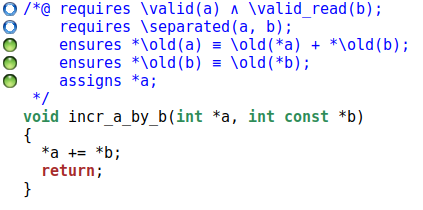
\includegraphics[scale=0.5]{2-2-2-incr_a_by_b-2.png}
\caption{Solved aliasing problems}
\label{fig:2-2-2-incr_a_by_b-2}
\end{figure}

We can notice that we do not consider the arithmetic overflow here, as
we do not focus on this question in this section. However, if this
function was part of a complete program, it would be necessary to define
the context of use of this function and the precondition guaranteeing
the absence of overflow.

\section{Behaviors}\label{behaviors}

Sometimes, a function can have behaviors that can be quite different
depending on the input. Typically, a function can receive a pointer to
an optional resource: if the pointer is \texttt{NULL}, we will have a
certain behavior, which will be different of the behavior expected when
the pointer is not \texttt{NULL}.

We have already seen a function that have different behaviors: the
\texttt{abs} function. We will use it again to illustrate behaviors. We
have two behaviors for the \texttt{abs} function: either the input is
positive or it is negative.

Behaviors allow us to specify the different cases for postconditions. We
introduce them using the \texttt{behavior} keyword. Each behavior will
have a name, the assumptions we have for the given case introduced with
the clause \texttt{assumes} and the associated postcondition. Finally,
we can ask WP to verify that behaviors are disjoint (to guarantee
determinism) and complete.

Behaviors are disjoint if for any (valid) input of the function, it
corresponds to the assumption (\texttt{assumes}) of a single behavior.
Behaviors are complete if any (valid) input of the function corresponds
to at least one behavior.

For example, for \texttt{abs} we can write the specification presented
in Figure~\ref{fig:3-3-0-abs}.

\begin{figure}
  \centering
\begin{footnotesize}\begin{Shaded}
\begin{Highlighting}[]
\CommentTok{/*@}
\CommentTok{  requires val > INT_MIN;}
\CommentTok{  assigns  \textbackslash{}nothing;}

\CommentTok{  behavior pos:}
\CommentTok{    assumes 0 <= val;}
\CommentTok{    ensures \textbackslash{}result == val;}
\CommentTok{  }
\CommentTok{  behavior neg:}
\CommentTok{    assumes val < 0;}
\CommentTok{    ensures \textbackslash{}result == -val;}
\CommentTok{ }
\CommentTok{  complete behaviors;}
\CommentTok{  disjoint behaviors;}
\CommentTok{*/}
\DataTypeTok{int} \NormalTok{abs(}\DataTypeTok{int} \NormalTok{val)\{}
  \KeywordTok{if}\NormalTok{(val < }\DecValTok{0}\NormalTok{) }\KeywordTok{return} \NormalTok{-val;}
  \KeywordTok{return} \NormalTok{val;}
\NormalTok{\}}
\end{Highlighting}
\end{Shaded}\end{footnotesize}
\caption{A specification using behaviors for \texttt{abs}}
\label{fig:3-3-0-abs}
\end{figure}

It can be useful to experiment two possibilities to understand the exact
meaning of \texttt{complete} and \texttt{disjoint}:

\begin{itemize}
\tightlist
\item
  replace the assumption of \texttt{pos} with
  \texttt{val\ \textgreater{}\ 0}, in this case, behaviors will be
  disjoint but incomplete (we will miss \texttt{val\ ==\ 0}),
\item
  replace the assumption of \texttt{neg} with
  \texttt{val\ \textless{}=\ 0}, in this case, behaviors will be
  complete but not disjoint (we will have two assumptions corresponding
  to \texttt{val\ ==\ 0}.
\end{itemize}

\clearpage

\begin{zdsalertblock}{Warning}
  Even if \texttt{assigns} is a postcondition, indicating different assigns
  in each behavior is currently not well-handled by WP. If we need to specify
  this, we will:
  \begin{itemize}
  \item put our \texttt{assigns} before the behaviors (as we have done in our
    example) with all potentially modified non-local element,
  \item add in post-condition of each behaviors the elements that are in fact
    not modified by indicating their new value to be equal to the
    \texttt{\textbackslash{}old} one.
  \end{itemize}
\end{zdsalertblock}

Behaviors are useful to simplify the writing of specifications when
functions can have very different behaviors depending on their input.
Without them, specification would be defined using implications
expressing the same idea but harder to write and read (which would be
error-prone).

On the other hand, the translation of completeness and disjointness
would be necessarily written by hand which would be tedious and again
error-prone.

\section{WP Modularity}\label{wp-modularity}

The end of this part will be dedicated to function call composition,
where we will start to have a closer look to WP. We will also have a
look to the way we can split our programs in different files when we
want to prove them using WP.

Our goal will be to prove the \texttt{max\_abs} function, that return
the maximum absolute value of two values:

\begin{footnotesize}\begin{Shaded}
\begin{Highlighting}[]
\DataTypeTok{int} \NormalTok{max_abs(}\DataTypeTok{int} \NormalTok{a, }\DataTypeTok{int} \NormalTok{b)\{}
  \DataTypeTok{int} \NormalTok{abs_a = abs(a);}
  \DataTypeTok{int} \NormalTok{abs_b = abs(b);}

  \KeywordTok{return} \NormalTok{max(abs_a, abs_b);}
\NormalTok{\}}
\end{Highlighting}
\end{Shaded}\end{footnotesize}

Let us start by (over-)splitting the function we already proved in pairs
header/source for \texttt{abs} and \texttt{max}. We will obtain, for
\texttt{abs} the files presented in Figure~\ref{fig:3-4-hd} and
\ref{fig:3-4-src}.

\begin{figure}
  \centering
\begin{footnotesize}\begin{Shaded}
\begin{Highlighting}[]
\CommentTok{#ifndef _ABS}
\CommentTok{#define _ABS}

\CommentTok{#include <limits.h>}

\CommentTok{/*@}
\CommentTok{  requires val > INT_MIN;}
\CommentTok{  assigns  \textbackslash{}nothing;}

\CommentTok{  behavior pos:}
\CommentTok{    assumes 0 <= val;}
\CommentTok{    ensures \textbackslash{}result == val;}
\CommentTok{  }
\CommentTok{  behavior neg:}
\CommentTok{    assumes val < 0;}
\CommentTok{    ensures \textbackslash{}result == -val;}
\CommentTok{ }
\CommentTok{  complete behaviors;}
\CommentTok{  disjoint behaviors;}
\CommentTok{*/}
\DataTypeTok{int} \NormalTok{abs(}\DataTypeTok{int} \NormalTok{val);}

\CommentTok{#endif}
\end{Highlighting}
\end{Shaded}\end{footnotesize}
\caption{Header for \texttt{abs}}
\label{fig:3-4-hd}
\end{figure}

\begin{figure}
  \centering
\begin{footnotesize}\begin{Shaded}
\begin{Highlighting}[]
\CommentTok{#include "abs.h"}

\DataTypeTok{int} \NormalTok{abs(}\DataTypeTok{int} \NormalTok{val)\{}
  \KeywordTok{if}\NormalTok{(val < }\DecValTok{0}\NormalTok{) }\KeywordTok{return} \NormalTok{-val;}
  \KeywordTok{return} \NormalTok{val;}
\NormalTok{\}}
\end{Highlighting}
\end{Shaded}\end{footnotesize}
\caption{Source file for \texttt{abs}}
\label{fig:3-4-src}
\end{figure}

We can notice that we put our function contract inside the header file.
The goal is to be able to import the specification at the same time than
the declaration when we need it in another file. Indeed, WP will need it
to be able to prove that the precondition of the function is verified
when we call it.

We can create a file using the same format for the \texttt{max}
function. In both cases, we can open the source file (we do not need to
specify header files in the command line) with Frama-C and notice that
the specification is indeed associated to the function and that we prove
it.

Now, we can prepare our files for the \texttt{max\_abs} function with
the header in Figure~\ref{fig:3-4-hd2} and its source file in
Figure~\ref{fig:3-4-src2}.

\begin{figure}
  \centering
\begin{footnotesize}\begin{Shaded}
\begin{Highlighting}[]
\CommentTok{#ifndef _MAX_ABS}
\CommentTok{#define _MAX_ABS}

\DataTypeTok{int} \NormalTok{max_abs(}\DataTypeTok{int} \NormalTok{a, }\DataTypeTok{int} \NormalTok{b);}

\CommentTok{#endif}
\end{Highlighting}
\end{Shaded}\end{footnotesize}
\caption{Header for \texttt{max\_abs}}
\label{fig:3-4-hd2}
\end{figure}

\begin{figure}
  \centering
\begin{footnotesize}\begin{Shaded}
\begin{Highlighting}[]
\CommentTok{#include "max_abs.h"}
\CommentTok{#include "max.h"}
\CommentTok{#include "abs.h"}

\DataTypeTok{int} \NormalTok{max_abs(}\DataTypeTok{int} \NormalTok{a, }\DataTypeTok{int} \NormalTok{b)\{}
  \DataTypeTok{int} \NormalTok{abs_a = abs(a);}
  \DataTypeTok{int} \NormalTok{abs_b = abs(b);}

  \KeywordTok{return} \NormalTok{max(abs_a, abs_b);}
\NormalTok{\}}
\end{Highlighting}
\end{Shaded}\end{footnotesize}
\caption{Source file for \texttt{max\_abs}}
\label{fig:3-4-src2}
\end{figure}

We can open the source file in Frama-C. If we look at the side panel, we
can see that the header files we have included in \texttt{abs\_max}
correctly appear and if we look at the function contracts for them, we
can see some blue and green bullets as illustrated by
Figure~\ref{fig:2-4-max_abs}.

\begin{figure}[htbp]
\centering
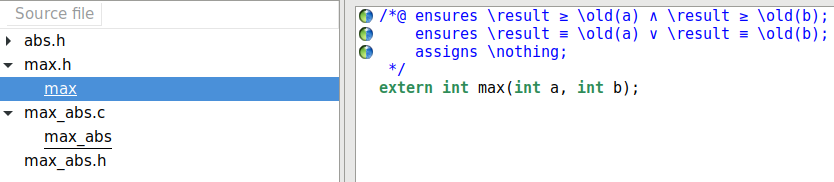
\includegraphics[scale=0.5]{2-4-max_abs.png}
\caption{The contract of \texttt{max} is assumed to be valid}
\label{fig:2-4-max_abs}
\end{figure}

These bullets indicate that, since we do not have the implementation,
they are assumed to be true. It is an important strength of the
deductive proof of programs compared to some other formal methods:
function are verified isolated from each other.

When we are not currently performing the proof of a function, its
specification is considered to be correct: we do not try to prove it
when we are proving another function, we will only verify that the
precondition is correctly established when we call it. It provides very
modular proofs and specifications that are therefore more reusable. Of
course, if our proof rely on the specification of another function, it
must be provable to ensure that the proof of the program is complete.
But, we can also consider that we trust a function that comes from an
external library that we do not want to prove (or for which we do not
even have the source code).

The careful reader could specify and prove the \texttt{max\_abs}
function.

A solution is provided there (we also add the implementation as a
reminder):

\begin{footnotesize}\begin{Shaded}
\begin{Highlighting}[]
\CommentTok{/*@}
\CommentTok{  requires a > INT_MIN;}
\CommentTok{  requires b > INT_MIN;}

\CommentTok{  assigns \textbackslash{}nothing;}

\CommentTok{  ensures \textbackslash{}result >= 0;}
\CommentTok{  ensures \textbackslash{}result >= a && \textbackslash{}result >= -a && \textbackslash{}result >= b && \textbackslash{}result >= -b;}
\CommentTok{  ensures \textbackslash{}result == a || \textbackslash{}result == -a || \textbackslash{}result == b || \textbackslash{}result == -b;}
\CommentTok{*/}
\DataTypeTok{int} \NormalTok{abs_max(}\DataTypeTok{int} \NormalTok{a, }\DataTypeTok{int} \NormalTok{b)\{}
  \DataTypeTok{int} \NormalTok{abs_a = abs(a);}
  \DataTypeTok{int} \NormalTok{abs_b = abs(b);}

  \KeywordTok{return} \NormalTok{max(abs_a, abs_b);}
\NormalTok{\}}
\end{Highlighting}
\end{Shaded}\end{footnotesize}

During this part of the tutorial, we have studied how we can specify
functions using contracts, composed of a pre and a post-condition, as
well as some features ACSL provides to express those properties. We have
also seen why it is important to be precise when we specify and how the
introduction of behaviors can help us to write more understandable and
concise specification.

However, we do not have studied one important point: the specification
of loops. Before that, we should have a closer look to the way WP works.

\chapter{Basic instructions and control
structures}\label{basic-instructions-and-control-structures}

\begin{zdsblock}{Information}
  This part is more formal than what we have seen so far. If the reader
  wishes to concentrate on the usage of the tool, he can skip the
  introduction and the first two sections (about the basic instructions
  and the bonus training) of this chapter. If what we presented so far has
  been difficult for the reader from a formal point of view,
  it is well possible to reserve the introduction and the two
  sections for a later reading.

  The sections on loops, however, are indispensable. We will highlight
  the more formal parts of these sections.
\end{zdsblock}

We will associate with every C programming construct

\begin{itemize}
\tightlist
\item
  the corresponding inference rule together,
\item
  its governing rule from the weakest precondition calculus and
\item
  examples that show its usage.
\end{itemize}

Not necessarily in that order and sometimes only with a loose connection
to the tool. Since the first rules are quite simple, we will discuss
them in a fairly theoretical manner. Later on, however, our presentation
will rely more and more on the tool, in particular when we begin dealing
with loops.

\subsection{Inference rules}\label{inference-rules}

An inference rule is of the form

\begin{center} \(\dfrac{P_1 \quad ... \quad P_n}{C}\) \end{center}

and means that in order to assure that the conclusion C is true, first
the truth of the premises \(P_1\), \ldots{}, and \(P_n\) has to be
established. In case that the rule has no premises

\begin{center} \(\dfrac{}{\quad C \quad}\) \end{center}

then nothing has to be assured in order to conclude the truth of \(C\).

On the other hand, in order to prove that a certain premise is true, it
might be necessary to employ other inference rules which would lead to
something like this:

\begin{center}
\(\dfrac{\dfrac{}{\quad P_1\quad} \quad \dfrac{P_{n_1}\quad P_{n_2}}{P_n}}{C}\)
\end{center}

This way, we obtain step by step the \emph{deduction tree} of our
reasoning. In our case, the premises and conclusions under consideration
will in general be \emph{Hoare triples}.

\subsection{Hoare triples}\label{hoare-triples-1}

We are now returning to concept of a Hoare triple:

\begin{center} \(\{ P \}\quad C\quad \{ Q \}\) \end{center}

In the beginning of this tutorial we have seen that this triple
expresses the following: if the property \(P\) holds before the
execution of \(C\) and if \(C\) terminates, then the property \(Q\)
holds too. For example, if we take up again our (slightly modified)
program for the computation of the absolute value:

\begin{footnotesize}\begin{Shaded}
\begin{Highlighting}[]
\CommentTok{/*@}
\CommentTok{  ensures \textbackslash{}result >= 0;}
\CommentTok{  ensures (val >= 0 ==> \textbackslash{}result == val ) && (val <  0 ==> \textbackslash{}result == -val);}
\CommentTok{*/}
\DataTypeTok{int} \NormalTok{abs(}\DataTypeTok{int} \NormalTok{val)\{}
  \DataTypeTok{int} \NormalTok{res;}
  \KeywordTok{if}\NormalTok{(val < }\DecValTok{0}\NormalTok{) res = - val;}
  \KeywordTok{else}        \NormalTok{res = val;}

  \KeywordTok{return} \NormalTok{res;}
\NormalTok{\}}
\end{Highlighting}
\end{Shaded}\end{footnotesize}

The rules of Hoare logic tell us that in order to show that our program
satisfies its contract we have to verify the properties shown in the
braces. (We have omitted one postcondition in order to simplify the
presentation.)

\begin{footnotesize}\begin{Shaded}
\begin{Highlighting}[]
\DataTypeTok{int} \NormalTok{abs(}\DataTypeTok{int} \NormalTok{val)\{}
  \DataTypeTok{int} \NormalTok{res;}
\CommentTok{// \{ P \}}
  \KeywordTok{if}\NormalTok{(val < }\DecValTok{0}\NormalTok{)\{}
\CommentTok{// \{  (val < 0) && P \}}
    \NormalTok{res = - val;}
\CommentTok{// \{ \textbackslash{}at(val, Pre) >= 0 ==> res == val && \textbackslash{}at(val, Pre) < 0 ==> res == -val \}}
  \NormalTok{\} }\KeywordTok{else} \NormalTok{\{}
\CommentTok{// \{ !(val < 0) && P \}}
    \NormalTok{res = val;}
\CommentTok{// \{ \textbackslash{}at(val, Pre) >= 0 ==> res == val && \textbackslash{}at(val, Pre) < 0 ==> res == -val \}}
  \NormalTok{\}}
\CommentTok{// \{ \textbackslash{}at(val, Pre) >= 0 ==> res == val && \textbackslash{}at(val, Pre) < 0 ==> res == -val \}}

  \KeywordTok{return} \NormalTok{res;}
\NormalTok{\}}
\end{Highlighting}
\end{Shaded}\end{footnotesize}

Yet, Hoare logic does not tell us how we can automatically obtain the
property \texttt{P} of our program \texttt{abs}. Dijkstra's
\emph{weakest-precondition calculus}, on the other hand, allows us to
compute from a given postcondition \(Q\) and a code snippet \(C\) the
minimal precondition \(P\) that ensures \(Q\) after the execution of
\(C\). We are thus in a position to determine for our example
\texttt{abs} the desired property \texttt{P}.

In this chapter we present the different cases of the function \(wp\)
which, starting from a given postcondition and a program (or statement),
computes the \emph{weakest} precondition that allows us to establish the
validity of the postcondition. We will use the following notation to
define the computation that corresponds to one ore several statements:

\(wp(Instruction(s), Post) := WeakestPrecondition\)

\clearpage
The function \(wp\) will guarantee that the Hoare triple

\begin{center} \(\{\ wp(C,Q)\ \}\quad C\quad \{ Q \}\) \end{center}

really is a valid triple.

We will thereby often use ACSL assertions in order to represent the
upcoming concepts:

\begin{footnotesize}\begin{Shaded}
\begin{Highlighting}[]
\CommentTok{//@ assert my_property;}
\end{Highlighting}
\end{Shaded}\end{footnotesize}

These assertions correspond in fact to possible intermediate steps for
the properties in our Hoare triples. We can, for example, replace the
properties of our function \texttt{abs} by corresponding ACSL assertions
(we have omitted here the property \texttt{P} because it is just
\texttt{true}):

\begin{footnotesize}\begin{Shaded}
\begin{Highlighting}[]
\DataTypeTok{int} \NormalTok{abs(}\DataTypeTok{int} \NormalTok{val)\{}
  \DataTypeTok{int} \NormalTok{res;}
  \KeywordTok{if}\NormalTok{(val < }\DecValTok{0}\NormalTok{)\{}
    \CommentTok{//@ assert val < 0 ;}
    \NormalTok{res = - val;}
    \CommentTok{//@ assert \textbackslash{}at(val, Pre) >= 0 ==> res == val && \textbackslash{}at(val, Pre) < 0 ==> res == -val ;}
  \NormalTok{\} }\KeywordTok{else} \NormalTok{\{}
    \CommentTok{//@ assert !(val < 0) ;}
    \NormalTok{res = val;}
    \CommentTok{//@ assert \textbackslash{}at(val, Pre) >= 0 ==> res == val && \textbackslash{}at(val, Pre) < 0 ==> res == -val ;}
  \NormalTok{\}}
  \CommentTok{//@ assert \textbackslash{}at(val, Pre) >= 0 ==> res == val && \textbackslash{}at(val, Pre) < 0 ==> res == -val ;}

  \KeywordTok{return} \NormalTok{res;}
\NormalTok{\}}
\end{Highlighting}
\end{Shaded}\end{footnotesize}

\section{Assignment, sequence and
conditional}\label{assignment-sequence-and-conditional}

\subsection{Assignment}\label{assignment}

Assignment is the most basic operation one can have in language (leaving
aside the ``do nothing'' operation that is not particularly
interesting). The weakest precondition calculus associates the following
computation to an assignment operation;

\begin{center} \(wp(x = E , Post) := Post[x \leftarrow E]\)
\end{center}

Here the notation \(P[x \leftarrow E]\) means ``the property \(P\) where
\(x\) is replaced by \(E\)''. In our case this corresponds to ``the
postcondition \(Post\) where \(x\) is replaced by \(E\)''. The idea is
that the postcondition of an assignment of \(E\) to \(x\) can only be
true if replacing all occurrences of \(x\) in the formula by \(E\) is
true. For example:

\begin{footnotesize}\begin{Shaded}
\begin{Highlighting}[]
\CommentTok{// \{ P \}}
\NormalTok{x = }\DecValTok{43} \NormalTok{* c ;}
\CommentTok{// \{ x = 258 \}}
\end{Highlighting}
\end{Shaded}\end{footnotesize}

\begin{center} \(P = wp(x = 43*c , \{x = 258\}) = \{43*c = 258\}\)
\end{center}

The function \(wp\) allows us to compute as weakest precondition of the
the assignment the formula \(\{43*c = 258\}\), thus obtaining the
following Hoare triple:

\begin{footnotesize}\begin{Shaded}
\begin{Highlighting}[]
\CommentTok{// \{ 43*c = 258 \}}
\NormalTok{x = }\DecValTok{43} \NormalTok{* c ;}
\CommentTok{// \{ x = 258 \}}
\end{Highlighting}
\end{Shaded}\end{footnotesize}

In order to compute the precondition of the assignment we have replaced
each occurrence of \(x\) in the postcondition by the assigned value
\(E = 43*c\). If our program were of the form:

\begin{footnotesize}\begin{Shaded}
\begin{Highlighting}[]
\DataTypeTok{int} \NormalTok{c = }\DecValTok{6} \NormalTok{;}
\CommentTok{// \{ 43*c = 258 \}}
\NormalTok{x = }\DecValTok{43} \NormalTok{* c ;}
\CommentTok{// \{ x = 258 \}}
\end{Highlighting}
\end{Shaded}\end{footnotesize}

we could submit the formula " \(43*6 = 258\) " to our automatic prover
in order to determine whether it is really valid. The answer would of
course be ``yes'' because the property is easy to verify. If we had,
however, given the value 7 to the variable \texttt{c} the prover's reply
would be ``no'' since the formula \(43*7 = 258\) is not true.

Taking into account the weakest precondition calculus, we can now write
the inference rule for the Hoare triple of an assignment as

\begin{center}
\(\dfrac{}{\{Q[x \leftarrow E] \}\quad x = E \quad\{ Q \}}\)
\end{center}

We note that there is no precondition to verify. Does this mean that the
triple is necessarily true? Yes. However, it does not mean that the
precondition is respected by the program to which the assignment belongs
or that the precondition is at all possible. Here the automatic provers
come into play.

For example, we can ask Frama-C to verify the following line

\begin{footnotesize}\begin{Shaded}
\begin{Highlighting}[]
\DataTypeTok{int} \NormalTok{a = }\DecValTok{42}\NormalTok{;}
\CommentTok{//@ assert a == 42;}
\end{Highlighting}
\end{Shaded}\end{footnotesize}

which is, of course, directly proven by Qed, since it is a simple
applications of the assignment rule.

\begin{zdsblock}{Information}
  We remark that according to the C standard, an assignment is in fact an
  expression. This allows us, for example, to write
  \texttt{if(\ (a\ =\ foo())\ ==\ 42)}.
  In Frama-C, an assignment will always be treated as a statement. Indeed,
  if an assignment occurs within a larger expression, then the Frama-C
  preprocessor, while building the abstract syntax tree, systematically
  performs a \emph{normalization step} that produces a separate assignment
  statement.
\end{zdsblock}

\subsection{Composition of statements}\label{composition-of-statements}

For a statement to be valid, its precondition must allow us by means of
executing the said statement to reach the desired postcondition. Now we
would like to execute several statements one after another. Here the
idea is that the postcondition of the first statement is compatible with
the required precondition of the second statement and so on for the
third statement.

\clearpage
The inference rule that corresponds to this idea utilizes the following
Hoare triples:

\begin{center}
\(\dfrac{\{P\}\quad S1 \quad \{R\} \ \ \ \{R\}\quad S2 \quad \{Q\}}{\{P\}\quad S1 ;\ S2 \quad \{Q\}}\)
\end{center}

In order to verify the composed statement \(S1;\ S2\) we rely on an
intermediate property \(R\) that is at the same time the postcondition
of \(S1\) and the precondition of \(S2\). (Please note that \(S1\) and
\(S2\) are not necessarily simple statements; they themselves can be
composed statements.) The problem is, however, that nothing indicates us
how to determine the properties \(P\) and \(R\).

The weakest-precondition calculus now says us that the intermediate
property \(R\) can be computed as the weakest precondition of the second
statement. The property \(P\), on the other hand, then is computed as
the weakest precondition of the first statement. In other words, the
weakest precondition of the composed statement \(S1; S2\) is determined
as follows:

\begin{center} \(wp(S1;\ S2 , Post) := wp(S1, wp(S2, Post) )\)
\end{center}

The WP plugin of Frama-C performs all these computations for us. Thus,
we do not have to write the intermediate properties as ACSL assertions
between the lines of codes.

\begin{footnotesize}\begin{Shaded}
\begin{Highlighting}[]
\DataTypeTok{int} \NormalTok{main()\{}
  \DataTypeTok{int} \NormalTok{a = }\DecValTok{42}\NormalTok{;}
  \DataTypeTok{int} \NormalTok{b = }\DecValTok{37}\NormalTok{;}

  \DataTypeTok{int} \NormalTok{c = a+b; }\CommentTok{// i:1}
  \NormalTok{a -= c;      }\CommentTok{// i:2}
  \NormalTok{b += a;      }\CommentTok{// i:3}

  \CommentTok{//@assert b == 0 && c == 79;}
\NormalTok{\}}
\end{Highlighting}
\end{Shaded}\end{footnotesize}

\subsubsection{Proof tree}\label{proof-tree}

When we have more than two statements, we can consider the last
statement as second statement of our rule and all the preceding ones as
first statement. This way we traverse step by step backwards the
statements in our reasoning. With the previous program this looks like:

\begin{center}
\begin{tabular}{ccc}
  $\{P\}\quad i_1 ; \quad \{Q_{-2}\}$ & $\{Q_{-2}\}\quad i_2 ; \quad \{Q_{-1}\}$ & \\
  \cline{1-2}
  \multicolumn{2}{c}{$\{P\}\quad i\_1 ; \quad i\_2 ; \quad \{Q_{-1}\}$} & $\{Q_{-1}\} \quad i_3 ; \quad \{Q\}$\\
  \hline
  \multicolumn{3}{c}{$\{P\}\quad i\_1 ; \quad i\_2 ; \quad i\_3; \quad \{ Q \}$}
\end{tabular}
\end{center}

The weakest-precondition calculus allows us to construct the property
\(Q_{-1}\) starting from the property \(Q\) and statement \(i_3\) which
in turn enables us to derive the property \(Q_{-2}\) from the property
\(Q_{-1}\) and statement \(i_2\). Finally, \(P\) can be determined from
\(Q_{-2}\) and \(i_1\).

Now that we can verify programs that consists of several statements it
is time to add some structure to them.

\subsection{Conditional rule}\label{conditional-rule}

For a conditional statement to be true, one must be able to reach the
postcondition through both branches. Of course, for both branches the
same precondition (of the conditional statement) must hold. In addition
we have that in the if-branch the condition is true while in the
else-branch it is false.

We therefore have, as in the case of composed statements, two facts to
verify (in order to avoid confusion we are using here the syntax
\(if\ B\ then\ S1\ else\ S2\)):

\begin{center}
\(\dfrac{\{P \wedge B\}\quad S1\quad \{Q\} \quad \quad \{P \wedge \neg B\}\quad S2\quad \{Q\}}{\{P\}\quad if\quad B\quad then\quad S1\quad else\quad S2 \quad \{Q\}}\)
\end{center}

Our two premises are therefore that we can both in the if-branch and the
else-branch reach the postcondition from the precondition.

The result of the weakest-precondition calculus for a conditional
statement reads as follows:

\begin{center}
\(wp(if\ B\ then\ S1\ else\ S2 , Post) := (B \Rightarrow wp(S1, Post)) \wedge (\neg B \Rightarrow wp(S2, Post))\)
\end{center}

This means that the condition \(B\) has to imply the weakest
precondition of \(S1\) in order to safely arrive at the postcondition.
Analogously, the negation of \(B\) must imply the weakest precondition
of \(S2\).

\subsubsection{Empty else-branch}\label{empty-else-branch}

Following this definition we obtain for case of an empty else-branch the
following rule by simply replacing the statement \(S2\) by the empty
statement \texttt{skip}.

\begin{center}
\(\dfrac{\{P \wedge B\}\quad S1\quad \{Q\} \quad \quad \{P \wedge \neg B\}\quad skip\quad \{Q\}}{\{P\}\quad if\quad B\quad then\quad S1\quad else\quad skip \quad \{Q\}}\)
\end{center}

The triple for \texttt{else} is:

\begin{center} \(\{P \wedge \neg B\}\quad skip\quad \{Q\}\)
\end{center}

which means that we need to ensure:

\begin{center} \(P \wedge \neg B \Rightarrow Q\) \end{center}

In short, if the condition \(B\) of \texttt{if} is false, this means
that the postcondition of the complete conditional statement is already
established before entering the else-branch (since it does not do
anything).

As an example, we consider the following code snippet where we reset a
variable \(c\) to a default value in case it had not been properly
initialized by the user.

\begin{footnotesize}\begin{Shaded}
\begin{Highlighting}[]
\DataTypeTok{int} \NormalTok{c;}

\CommentTok{// ... some code ...}

\KeywordTok{if}\NormalTok{(c < }\DecValTok{0} \NormalTok{|| c > }\DecValTok{15}\NormalTok{)\{}
  \NormalTok{c = }\DecValTok{0}\NormalTok{;}
\NormalTok{\}}
\CommentTok{//@ assert 0 <= c <= 15;}
\end{Highlighting}
\end{Shaded}\end{footnotesize}

Let

\(wp(if \neg (c \in [0;15])\ then\ c := 0, \{c \in [0;15]\})\)

\(:= (\neg (c \in [0;15])\Rightarrow wp(c := 0, \{c \in [0;15]\})) \wedge (c \in [0;15]\Rightarrow wp(skip, \{c \in [0;15]\}))\)

\(= (\neg (c \in [0;15]) \Rightarrow 0 \in [0;15]) \wedge (c \in [0;15] \Rightarrow c \in [0;15])\)

\(= (\neg (c \in [0;15]) \Rightarrow true) \wedge true\)

The property can be verified: independent of the evaluation of
\(\neg (c \in [0;15])\), the implication will hold.

\section{{[}Bonus Stage{]} Consequence and
constancy}\label{bonus-stage-consequence-and-constancy}

\subsection{Consequence rule}\label{consequence-rule}

It can sometimes be useful to strengthen a postcondition or to weaken a
precondition. If the former will often be established by us to
facilitate the work of the prover, the second is more often verified by
the tool as the result of computing the weakest precondition.

The inference rule of Hoare logic is the following:

\begin{center}\(\dfrac{P \Rightarrow WP \quad \{WP\}\quad c\quad \{SQ\} \quad SQ \Rightarrow Q}{\{P\}\quad c \quad \{Q\}}\)\end{center}

(We remark that the premises here are not only Hoare triples but also
formulas to verify.)

For example, if our post-condition is too complex, it may generate a
weaker precondition that is, however, too complicated, thus making the
work of provers more difficult. We can then create a simpler
intermediate postcondition \(SQ\), that is, however, stricter and
implies the real postcondition. This is the part \(SQ \Rightarrow Q\).

Conversely, the calculation of the precondition will usually generate a
complicated and often weaker formula than the precondition we want to
accept as input. In this case, it is our tool that will check the
implication between what we want and what is necessary for our code to
be valid. Th is is the part \(P \Rightarrow WP\).

We can illustrate this with the following code. Note that here the code
could be proved by WP without the weakening and strengthening of
properties because the code is very simple, it is just to illustrate the
rule of consequence.

\clearpage

\begin{footnotesize}\begin{Shaded}
\begin{Highlighting}[]
\CommentTok{/*@}
\CommentTok{  requires P: 2 <= a <= 8;}
\CommentTok{  ensures  Q: 0 <= \textbackslash{}result <= 100 ;}
\CommentTok{  assigns  \textbackslash{}nothing ;}
\CommentTok{*/}
\DataTypeTok{int} \NormalTok{constrained_times_10(}\DataTypeTok{int} \NormalTok{a)\{}
  \CommentTok{//@ assert P_imply_WP: 2 <= a <= 8 ==> 1 <= a <= 9 ;}
  \CommentTok{//@ assert WP:         1 <= a <= 9 ;}

  \DataTypeTok{int} \NormalTok{res = a * }\DecValTok{10}\NormalTok{;}

  \CommentTok{//@ assert SQ:         10 <= res <= 90 ;}
  \CommentTok{//@ assert SQ_imply_Q: 10 <= res <= 90 ==> 0 <= res <= 100 ;}

  \KeywordTok{return} \NormalTok{res;}
\NormalTok{\}}
\end{Highlighting}
\end{Shaded}\end{footnotesize}

(Note: We have omitted here the control of integer overflow.)

Here we want to have a result between 0 and 100. But we know that the
code will not produce a result outside the bounds of 10 and 90. So we
strengthen the postcondition with an assertion that at the end
\texttt{res}, the result, is between 0 and 90. The calculation of the
weakest precondition of this property together with the assignment
\texttt{res\ =\ 10\ *\ a} yields a weaker precondition
\texttt{1\ \textless{}=\ a\ \textless{}=\ 9} and we know that
\texttt{2\ \textless{}\ =\ a\ \textless{}=\ 8} gives us the desired
guarantee.

When there are difficulties to carry out a proof on more complex code,
then it is often helpful to write assertions that produce stronger, yet
easier to verify, postconditions. Note that in the previous code, the
lines \texttt{P\_imply\_WP} and\texttt{SQ\_imply\_Q} are never used
because this is the default reasoning of WP. They are just here for
illustrating the rule.

\subsection{Constancy rule}\label{constancy-rule}

Certain sequences of instructions may concern and involve different
variables. Thus, we may initialize and manipulate a certain number of
variables, begin to use some of them for a time, before using other
variables. When this happens, we want our tool to be concerned only with
variables that are susceptible to change in order to obtain the simplest
possible properties.

The rule of inference that defines this reasoning is the following:

\begin{center}
\(\dfrac{\{P\}\quad c\quad \{Q\}}{\{P \wedge R\}\quad c\quad \{Q \wedge R\}}\)
\end{center}

where \(c\) does not modify any input variable in \(R\). In other words:
``To check the triple, let's get rid of the parts of the formula that
involves variables that are not influence by \(c\) and prove the new
triple.'' However, we must be careful not to delete too much
information, since this could mean that we are not able to prove our
properties.

\clearpage 
As an example,let us consider the following code (here gain, we ignore
potential integer overflows):

\begin{footnotesize}\begin{Shaded}
\begin{Highlighting}[]
\CommentTok{/*@}
\CommentTok{  requires a > -99 ;}
\CommentTok{  requires b > 100 ;}
\CommentTok{  ensures  \textbackslash{}result > 0 ;}
\CommentTok{  assigns  \textbackslash{}nothing ;}
\CommentTok{*/}
\DataTypeTok{int} \NormalTok{foo(}\DataTypeTok{int} \NormalTok{a, }\DataTypeTok{int} \NormalTok{b)\{}
  \KeywordTok{if}\NormalTok{(a >= }\DecValTok{0}\NormalTok{)\{}
    \NormalTok{a++ ;}
  \NormalTok{\} }\KeywordTok{else} \NormalTok{\{}
    \NormalTok{a += b ;}
  \NormalTok{\}}
  \KeywordTok{return} \NormalTok{a ;}
\NormalTok{\}}
\end{Highlighting}
\end{Shaded}\end{footnotesize}

If we look at the code of the \texttt{if} block, we notice that it does
not use the variable \texttt{b}. Thus, we can completely omit the
properties about \texttt{b} in order to prove that \texttt{a} will be
strictly greater than 0 after the execution of the block:

\begin{footnotesize}\begin{Shaded}
\begin{Highlighting}[]
\CommentTok{/*@}
\CommentTok{  requires a > -99 ;}
\CommentTok{  requires b > 100 ;}
\CommentTok{  ensures  \textbackslash{}result > 0 ;}
\CommentTok{  assigns  \textbackslash{}nothing ;}
\CommentTok{*/}
\DataTypeTok{int} \NormalTok{foo(}\DataTypeTok{int} \NormalTok{a, }\DataTypeTok{int} \NormalTok{b)\{}
  \KeywordTok{if}\NormalTok{(a >= }\DecValTok{0}\NormalTok{)\{}
    \CommentTok{//@ assert a >= 0; // no mentioning of b}
    \NormalTok{a++ ;}
  \NormalTok{\} }\KeywordTok{else} \NormalTok{\{}
    \NormalTok{a += b ;}
  \NormalTok{\}}
  \KeywordTok{return} \NormalTok{a ;}
\NormalTok{\}}
\end{Highlighting}
\end{Shaded}\end{footnotesize}

On the other hand, in the \texttt{else} block, even if \texttt{b} were
not modified, formulating properties only about \texttt{a} would render
a proof impossible for humans. The code would be:

\begin{footnotesize}\begin{Shaded}
\begin{Highlighting}[]
\CommentTok{/*@}
\CommentTok{  requires a > -99 ;}
\CommentTok{  requires b > 100 ;}
\CommentTok{  ensures  \textbackslash{}result > 0 ;}
\CommentTok{  assigns  \textbackslash{}nothing ;}
\CommentTok{*/}
\DataTypeTok{int} \NormalTok{foo(}\DataTypeTok{int} \NormalTok{a, }\DataTypeTok{int} \NormalTok{b)\{}
  \KeywordTok{if}\NormalTok{(a >= }\DecValTok{0}\NormalTok{)\{}
    \CommentTok{//@ assert a >= 0; // no mentioning of b}
    \NormalTok{a++ ;}
  \NormalTok{\} }\KeywordTok{else} \NormalTok{\{}
    \CommentTok{//@ assert a < 0 && a > -99 ; // no mentioning of b}
    \NormalTok{a += b ;}
  \NormalTok{\}}
  \KeywordTok{return} \NormalTok{a ;}
\NormalTok{\}}
\end{Highlighting}
\end{Shaded}\end{footnotesize}

In the \texttt{else} block, knowing that\texttt{a} lies between -99 and
0, but knowing nothing about \texttt{b}, we could hardly know if the
operation \texttt{a\ +\ =\ b} produces a result that is greater than 0.

The WP plug-in will, of course, prove the function without problems,
since it produces by itself the properties that are necessary for the
proof. In fact, the analysis which variables are necessary or not (and,
consequently, the application of the constancy rule) is conducted
directly by WP.

Let us finally remark that the constancy rule is an instance of the
consequence rule:

\begin{center}\(\dfrac{P \wedge R \Rightarrow P \quad \{P\}\quad c\quad \{Q\} \quad Q \Rightarrow Q \wedge R}{\{P \wedge R\}\quad c\quad \{Q \wedge R\}}\)
\end{center}

If the variables of \(R\) have not been modified by the operation
(which, on the other hand, may modify the variables of \(P\) to produce
\(Q\)), then the properties \(P \ wedge R \ Rightarrow P\) and
\(Q \ Rightarrow Q \ wedge R\) hold.

\section{Loops}\label{loops}

Loops needs a particular treatment in deductive verification of
programs. These are the only control structures that will require an
important work from us. We cannot avoid this because without loops, it
is difficult to write and prove interesting programs.

Before we look at the way we specify loop, we can answer to a rightful
question: why are loops so complex?

\subsection{Induction and invariant}\label{induction-and-invariant}

The nature of loops makes their analysis complex. When we perform our
backward reasoning, we need a rule to determine from a post-condition,
what is the precondition to a given sequence of instructions. Here, the
problem is that we cannot \emph{a priori} deduce how many times a loop
will iterate, and consequently, we cannot know neither how many times
variables will be modified.

we will then proceed using an inductive reasoning. We have to find a
property that is true before we start to execute the loop and that, if
it is true at the beginning of an iteration, remains true at the end
(and that is consequently true at the beginning of the next iteration).

This type of property is called a loop invariant. A loop invariant is a
property that must be true before and after each loop instruction. For
example with the following loop:

\begin{footnotesize}\begin{Shaded}
\begin{Highlighting}[]
\KeywordTok{for}\NormalTok{(}\DataTypeTok{int} \NormalTok{i = }\DecValTok{0} \NormalTok{; i < }\DecValTok{10} \NormalTok{; ++i)\{ }\CommentTok{/* */} \NormalTok{\}}
\end{Highlighting}
\end{Shaded}\end{footnotesize}

The property \(0 <= i <= 10\) is a loop invariant. The property
\(-42 <= i <= 42\) is also an invariant (even if it is far less
precise). The property \(0 < i <= 10\) is not an invariant because it is
not true at the beginning of the execution of the loop. The property
\(0 <= i < 10\) \textbf{is not a loop invariant}, it is not true at the
end of the last iteration that sets the value of \texttt{i} to \(10\).

To verify an invariant \(I\), WP will then produce the following
``reasoning'':

\begin{itemize}
\tightlist
\item
  verify that \(I\) is true at the beginning of the loop (establishment)
\item
  verify that if \(I\) is true before an iteration, then \(I\) is true
  after (preservation).
\end{itemize}

\subsubsection{{[}Formal{]} Inference rule}\label{formal-inference-rule}

Let us note the invariant \(I\), the inference rule corresponding to
loops is defined as follows:

\begin{center}
\(\dfrac{\{I \wedge B \}\ c\ \{I\}}{\{I\}\ while(B)\{c\}\ \{I \wedge \neg B\}}\)
\end{center}

And the weakest precondition calculus is the following:

\begin{center}
\(wp(while (B) \{ c \}, Post) := I \wedge ((B \wedge I) \Rightarrow wp(c, I)) \wedge ((\neg B \wedge I) \Rightarrow Post)\)
\end{center}

Let us detail this formula:

\begin{itemize}
\item
  \begin{enumerate}
  \def\labelenumi{(\arabic{enumi})}
  \tightlist
  \item
    the first \(I\) corresponds to the establishment of the invariant,
    in layman's terms, this is the ``precondition'' of the loop,
  \end{enumerate}
\item
  the second part of the conjunction
  (\((B \wedge I) \Rightarrow wp(c, I)\)) corresponds to the
  verification of the operation performed by the body of the loop:

  \begin{itemize}
  \item
    the precondition that we know of the loop body (let us note \(KWP\),
    ``Known WP'') is (\(KWP = B \wedge I\)). That is the fact we have
    entered the loop (\(B\) is true), and that the invariant is verified
    at this moment (\(I\), is true before we start the loop by (1), and
    we want to verify that it will be true at the end of the body of the
    loop in (2)),
  \item
    \begin{enumerate}
    \def\labelenumi{(\arabic{enumi})}
    \setcounter{enumi}{1}
    \tightlist
    \item
      it remains to verify that \(KWP\) implies the actual precondition*
      of the body of the loop (\(KWP \Rightarrow wp(c, Post)\)). What we
      want at the end of the loop is the preservation of the invariant
      \(I\) (\(B\) is maybe not true anymore however), formally
      \(KWP \Rightarrow wp(c, I)\), that is to say
      \((B \wedge I) \Rightarrow wp(c, I)\),
    \end{enumerate}
  \item
    * it corresponds to the application of the consequence rule
    previously explained.
  \end{itemize}
\item
  finally, the last part (\((\neg B \wedge I) \Rightarrow Post\))
  expresses the fact that when the loop ends(\(\neg B\)), and the
  invariant \(I\) has been maintained, it must imply that the wanted
  postcondition of the loop is
\end{itemize}

In this computation, we can notice that the \(wp\) function do not
indicate any way to obtain the invariant \(I\). We have to specify
ourselves this property about our loops.

\subsubsection{Back to the WP plugin}\label{back-to-the-wp-plugin}

There exist tools that can infer invariant properties (provided that
these properties are simple, automatic tools remains limited). It is not
the case for WP. We will have to manually annotate our programs to
specify the invariant of each loop. To find and write invariant for our
loops will always be the hardest part of our work when we want to prove
programs.

Indeed if, when there are no loops, the weakest precondition calculus
function can automatically provide the verifiable properties of our
programs, it is not the case for loop invariant properties for which we
do not have computation procedures. We have to find and express them
correctly, and depending on the algorithm, they can be quite subtle and
complex.

In order to specify a loop invariant, we add the following annotations
before the loop:

\begin{footnotesize}\begin{Shaded}
\begin{Highlighting}[]
\DataTypeTok{int} \NormalTok{main()\{}
  \DataTypeTok{int} \NormalTok{i = }\DecValTok{0}\NormalTok{;}
  
  \CommentTok{/*@}
\CommentTok{    loop invariant 0 <= i <= 30;}
\CommentTok{  */}
  \KeywordTok{while}\NormalTok{(i < }\DecValTok{30}\NormalTok{)\{}
    \NormalTok{++i;}
  \NormalTok{\}}
  \CommentTok{//@assert i == 30;}
\NormalTok{\}}
\end{Highlighting}
\end{Shaded}\end{footnotesize}

\begin{zdsalertblock}{Warning}
  \textbf{REMINDER} : The invariant is: i \textbf{\textless{}=} 30 !
\end{zdsalertblock}
  
Why? Because along the loop, \texttt{i} will be comprised between 0 and
\textbf{included} 30. 30 is indeed the value that allows us to leave the
loop. Moreover, one of the properties required by the weakest
precondition calculus is that when the loop condition is invalidated, by
knowing the invariant, we can prove the postcondition (Formally
\((\neg B \wedge I) \Rightarrow Post\)).

The postcondition of our loop is \texttt{i\ ==\ 30} and must be implied
by \(\neg\) \texttt{i\ \textless{}\ 30} \(\wedge\)
\texttt{0\ \textless{}=\ i\ \textless{}=\ 30}. Here, it is true since:
\texttt{i\ \textgreater{}=\ 30\ \&\&\ 0\ \textless{}=\ i\ \textless{}=\ 30\ ==\textgreater{}\ i\ ==\ 30}.
On the opposite, if we exclude the equality to 30, the postcondition
would be unreachable.

Again, we can have a look to the list of proof obligations in ``WP
Goals'' (illustrated by Figure~\ref{fig:3-3-1-i_30-1}).

\begin{figure}[htbp]
\centering
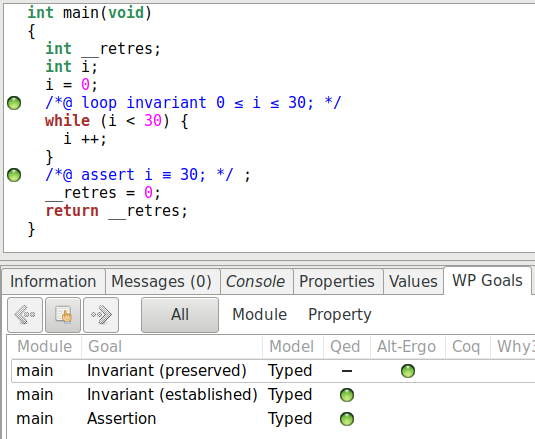
\includegraphics[scale=0.5]{3-3-1-i_30-1.png}
\caption{Proof obligations generated to verify our loop}
\label{fig:3-3-1-i_30-1}
\end{figure}

We note that WP produces two different proof obligations: the
establishment of the invariant and its preservation. WP produces exactly
the reasoning we previously described to prove the assertion. In recent
versions of Frama-C, Qed has become particularly aggressive and
powerful, and the generated proof obligation does not show these details
(showing directly ``True''). Using the option \texttt{-wp-no-simpl} at
start, we can however see these details (see Figure~\ref{fig:3-3-end_loop}).

\begin{figure}[htbp]
\centering
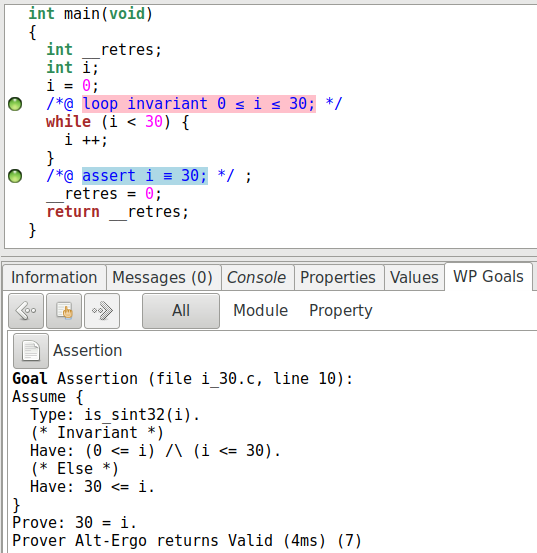
\includegraphics[scale=0.5]{3-3-sortie-boucle.png}
\caption{Proof of the assertion, knowing the invariant and the
  invalidation of the loop condition}
\label{fig:3-3-end_loop}
\end{figure}

But is our specification precise enough?

\begin{footnotesize}\begin{Shaded}
\begin{Highlighting}[]
\DataTypeTok{int} \NormalTok{main()\{}
  \DataTypeTok{int} \NormalTok{i = }\DecValTok{0}\NormalTok{;}
  \DataTypeTok{int} \NormalTok{h = }\DecValTok{42}\NormalTok{;}
  
  \CommentTok{/*@}
\CommentTok{    loop invariant 0 <= i <= 30;}
\CommentTok{  */}
  \KeywordTok{while}\NormalTok{(i < }\DecValTok{30}\NormalTok{)\{}
    \NormalTok{++i;}
  \NormalTok{\}}
  \CommentTok{//@assert i == 30;}
  \CommentTok{//@assert h == 42;}
\NormalTok{\}}
\end{Highlighting}
\end{Shaded}\end{footnotesize}

And the result is:

\begin{figure}[htbp]
  \centering
  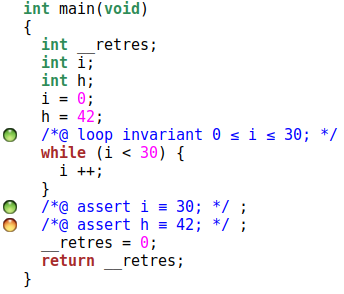
\includegraphics[scale=0.5]{3-3-boucle-effet-bord.png}
  \caption{Side-effects, again}
  \label{fig:3-3-loop-side-effect}
\end{figure}

It seems not (sse Figure~\ref{fig:3-3-loop-side-effect}).

\subsection{The assigns clause \ldots{} for
loops}\label{the-assigns-clause-for-loops}

In fact, considering loops, WP \textbf{only} reasons about what is
provided by the user to perform its reasoning. And here, the invariant
does not specify anything about the way the value of \texttt{h} is
modified (or not). We could specify the invariant of all program
variables, but it would be a lot of work. ACSL simply allows to add
\texttt{assigns} annotations for loops. Any other variable is considered
to keep its old value. For example:

\begin{footnotesize}\begin{Shaded}
\begin{Highlighting}[]
\DataTypeTok{int} \NormalTok{main()\{}
  \DataTypeTok{int} \NormalTok{i = }\DecValTok{0}\NormalTok{;}
  \DataTypeTok{int} \NormalTok{h = }\DecValTok{42}\NormalTok{;}
  
  \CommentTok{/*@}
\CommentTok{    loop invariant 0 <= i <= 30;}
\CommentTok{    loop assigns i;}
\CommentTok{  */}
  \KeywordTok{while}\NormalTok{(i < }\DecValTok{30}\NormalTok{)\{}
    \NormalTok{++i;}
  \NormalTok{\}}
  \CommentTok{//@assert i == 30;}
  \CommentTok{//@assert h == 42;}
\NormalTok{\}}
\end{Highlighting}
\end{Shaded}\end{footnotesize}

This time, we can establish the proof that the loop correctly behaves.
However, we cannot prove that it terminates. The loop invariant is not
enough to perform such a proof. For example, in our program, we could
modify the loop, removing the loop body:

\begin{footnotesize}\begin{Shaded}
\begin{Highlighting}[]
\CommentTok{/*@}
\CommentTok{  loop invariant 0 <= i <= 30;}
\CommentTok{  loop assigns i;}
\CommentTok{*/}
\KeywordTok{while}\NormalTok{(i < }\DecValTok{30}\NormalTok{)\{}
   
\NormalTok{\}}
\end{Highlighting}
\end{Shaded}\end{footnotesize}

The invariant is still verified, but we cannot prove that the loop ends:
it is infinite.

\subsection{Partial correctness and total correctness - Loop
variant}\label{partial-correctness-and-total-correctness---loop-variant}

In deductive verification, we find two types of correctness, the partial
correctness and the total correctness. In the first case, the
formulation of the correctness property is ``if the precondition is
valid, and \textbf{if} the computation terminates, then the
postcondition is valid''. In the second case, ``if the precondition is
valid, \textbf{then} the computation terminates and the postcondition is
valid''. By default, WP considers only partial correctness:

\begin{footnotesize}\begin{Shaded}
\begin{Highlighting}[]
\DataTypeTok{void} \NormalTok{foo()\{}
  \KeywordTok{while}\NormalTok{(}\DecValTok{1}\NormalTok{)\{\}}
  \CommentTok{//assert \textbackslash{}false;}
\NormalTok{\}}
\end{Highlighting}
\end{Shaded}\end{footnotesize}

If we try to verify this code activating the verification of absence of
RTE, we get the result presented in Figure~\ref{fig:3-3-infini}.

\begin{figure}[htbp]
  \centering
  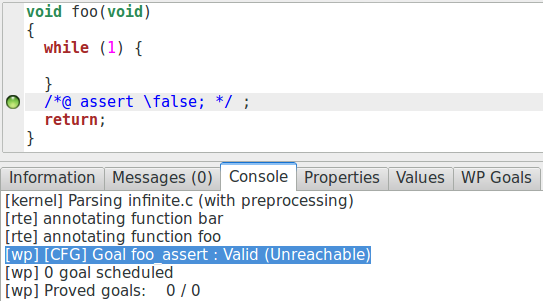
\includegraphics[scale=0.5]{3-3-infinite.png}
  \caption{Proof of false by non termination}
  \label{fig:3-3-infini}
\end{figure}

The assertion ``False'' is proved! For a very simple reason: since the
condition of the loop is ``True'' and no instruction of the loop body
allows to leave the loop, it will not terminate. As we are proving the
code with partial correctness, and as the execution does not terminate,
we can prove anything about the code that follows the non terminating
part of the code. However, if the termination is not trivially provable,
the assertion will probably not be proved.

\begin{zdsblock}{Information}
  Note that an (provably) unreachable assertion is always proved to be true:
  \begin{center}
    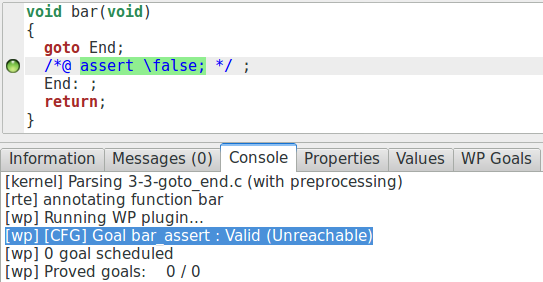
\includegraphics[scale=0.5]{3-3-goto_end.png}
  \end{center}
  And this is also the case when we trivially know that an instruction
  produces a runtime error (for example dereferencing \texttt{NULL}), or
  inserting ``False'' in post-condition as we have already seen with
  \texttt{abs} and the parameter \texttt{INT\_MIN}.
\end{zdsblock}

In order to prove the termination of a loop, we use the notion of loop
variant. The loop variant is not a property but a value. It is an
expression that involves the element modified by the loop and that
provides an upper bound to the number of iteration that have to be
executed by the loop at each iteration. Thus, it is an expression
greater or equal to 0, and that strictly decreases at each loop
iteration (it will also be verified by induction by WP).

\clearpage
If we take our previous example, we add the loop variant with this
syntax:

\begin{footnotesize}\begin{Shaded}
\begin{Highlighting}[]
\DataTypeTok{int} \NormalTok{main()\{}
  \DataTypeTok{int} \NormalTok{i = }\DecValTok{0}\NormalTok{;}
  \DataTypeTok{int} \NormalTok{h = }\DecValTok{42}\NormalTok{;}
  
  \CommentTok{/*@}
\CommentTok{    loop invariant 0 <= i <= 30;}
\CommentTok{    loop assigns i;}
\CommentTok{    loop variant 30 - i;}
\CommentTok{  */}
  \KeywordTok{while}\NormalTok{(i < }\DecValTok{30}\NormalTok{)\{}
    \NormalTok{++i;}
  \NormalTok{\}}
  \CommentTok{//@assert i == 30;}
  \CommentTok{//@assert h == 42;}
\NormalTok{\}}
\end{Highlighting}
\end{Shaded}\end{footnotesize}

Again, we can have a look to the generated proof obligations
(see Figure~\ref{fig:3-3-loop-ok}).

\begin{figure}[htbp]
\centering
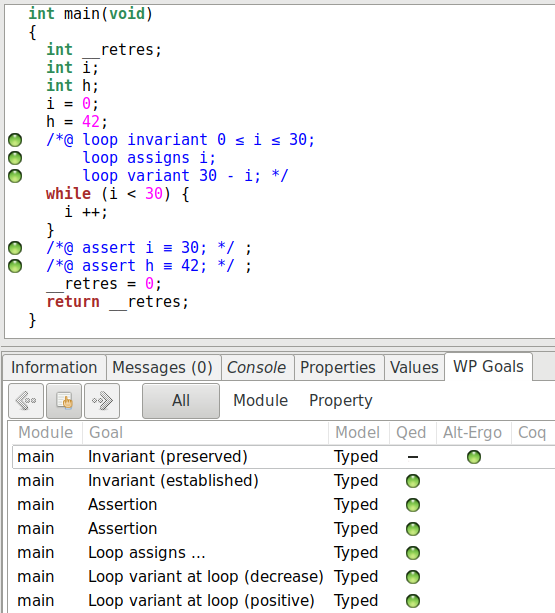
\includegraphics[scale=0.5]{3-3-boucle_complete.png}
\caption{Our loop entirely specified and proved}
\label{fig:3-3-loop-ok}
\end{figure}

The loop variant generates two proof obligations: verify that the value
specified in the variant is positive, and prove that it strictly
decreases during the execution of the loop. And if we delete the line of
code that increments \texttt{i}, WP cannot prove anymore that
\texttt{30\ -\ i} strictly decreases.

We can also note that being able to give a loop invariant does not
necessarily induce that we can give the exact number of remaining
iterations of the loop, as we do not always have a so precise knowledge
of the behavior of the program. We can for example build an example like
this one:
\clearpage
\begin{footnotesize}\begin{Shaded}
\begin{Highlighting}[]
\ErrorTok{#include <stddef.h>}

\CommentTok{/*@}
\CommentTok{  ensures min <= \textbackslash{}result <= max;}
\CommentTok{*/}
\NormalTok{size_t random_between(size_t min, size_t max);}

\DataTypeTok{void} \NormalTok{undetermined_loop(size_t bound)\{}
  \CommentTok{/*@}
\CommentTok{    loop invariant 0 <= i <= bound ;}
\CommentTok{    loop assigns i;}
\CommentTok{    loop variant i;}
\CommentTok{   */}
  \KeywordTok{for}\NormalTok{(size_t i = bound; i > }\DecValTok{0}\NormalTok{; )\{}
    \NormalTok{i -= random_between(}\DecValTok{1}\NormalTok{, i);}
  \NormalTok{\}}
\NormalTok{\}}
\end{Highlighting}
\end{Shaded}\end{footnotesize}

Here, at each iteration, we decrease the value of the variable
\texttt{i} by a value comprised between 1 and \texttt{i}. Thus, we can
ensure that the value of \texttt{i} is positive and strictly decreases
during each loop iteration, but we cannot say how many loop iteration
will be executed.

The loop variant is then only an upper bound on the number of iteration,
not an expression of their exact number.

\subsection{Create a link between post-condition and
invariant}\label{create-a-link-between-post-condition-and-invariant}

Let us consider the following specified program. Our goal is to prove
that this function returns the old value of \texttt{a} plus 10.

\begin{footnotesize}\begin{Shaded}
\begin{Highlighting}[]
\CommentTok{/*@}
\CommentTok{    ensures \textbackslash{}result == \textbackslash{}old(a) + 10;}
\CommentTok{*/}
\DataTypeTok{int} \NormalTok{add_10(}\DataTypeTok{int} \NormalTok{a)\{}
    \CommentTok{/*@}
\CommentTok{        loop invariant 0 <= i <= 10;}
\CommentTok{        loop assigns i, a;}
\CommentTok{        loop variant 10 - i;}
\CommentTok{    */}
    \KeywordTok{for} \NormalTok{(}\DataTypeTok{int} \NormalTok{i = }\DecValTok{0}\NormalTok{; i < }\DecValTok{10}\NormalTok{; ++i)}
        \NormalTok{++a;}

    \KeywordTok{return} \NormalTok{a;}
\NormalTok{\}}
\end{Highlighting}
\end{Shaded}\end{footnotesize}

\begin{figure}
\begin{footnotesize}\begin{Shaded}
\begin{Highlighting}[]
\CommentTok{/*@}
\CommentTok{    ensures \textbackslash{}result == \textbackslash{}old(a) + 10;}
\CommentTok{*/}
\DataTypeTok{int} \NormalTok{add_10(}\DataTypeTok{int} \NormalTok{a)\{}
    \NormalTok{++a;}
    \NormalTok{++a;}
    \NormalTok{++a;}
    \CommentTok{//...}
    \KeywordTok{return} \NormalTok{a;}
\NormalTok{\}}
\end{Highlighting}
\end{Shaded}\end{footnotesize}
\caption{Unrolled loop}
\label{fig:4-3-4-unrolled}
\end{figure}

The weakest precondition calculus does not allow to deduce information
that is not part of the loop invariant. In a code like the one presented
in Figure~\ref{fig:4-3-4-unrolled}, by reading the instructions backward
from the postcondition, we always keep all knowledge about \texttt{a}. On
the opposite, as we previously mentioned, outside the loop, WP only
considers the information provided by the invariant. Consequently, our
``add\_10'' function cannot be proved: the invariant does not say anything
about \texttt{a}. To create a link between the postcondition and the
invariant, we have to add this knowledge. See, for example, the code
illustrated by Figure~\ref{fig:4-3-4-comp_inv}.

\begin{figure}
\begin{footnotesize}\begin{Shaded}
\begin{Highlighting}[]
\CommentTok{/*@}
\CommentTok{    ensures \textbackslash{}result == \textbackslash{}old(a) + 10;}
\CommentTok{*/}
\DataTypeTok{int} \NormalTok{add_10(}\DataTypeTok{int} \NormalTok{a)\{}
    \CommentTok{/*@}
\CommentTok{        loop invariant 0 <= i <= 10;}
\CommentTok{        loop invariant a = \textbackslash{}old(a) + i; //< ADDED}
\CommentTok{        loop assigns i, a;}
\CommentTok{        loop variant 10 - i;}
\CommentTok{    */}
    \KeywordTok{for} \NormalTok{(}\DataTypeTok{int} \NormalTok{i = }\DecValTok{0}\NormalTok{; i < }\DecValTok{10}\NormalTok{; ++i)}
        \NormalTok{++a;}

    \KeywordTok{return} \NormalTok{a;}
\NormalTok{\}}
\end{Highlighting}
\end{Shaded}\end{footnotesize}
\caption{Strenghtened invariant}
\label{fig:4-3-4-comp_inv}
\end{figure}

\begin{zdsblock}{Information}
  This need can appear as a very strong constraint. This is not really the
  case. There exists strongly automated analysis that can compute loop
  invariant properties. For example, without a specification, an abstract
  interpretation would easily compute \texttt{0\ \textless{}=\ i\ \textless{}=\ 10}
  and \texttt{old(a)\ \textless{}=\ a\ \textless{}=\ \textbackslash{}old(a)+10}.
  However, it is often more difficult to compute the relations
  that exists between the different variables of a program, for
  example the equality expressed by the invariant we have
  added.
\end{zdsblock}

\section{Loops - Examples}\label{loops---examples}

\subsection{Examples with read-only
arrays}\label{examples-with-read-only-arrays}

Array is the most common data structure when we are working with loops.
It is then a good example base to exercise with loops, and these
examples allow to rapidly show interesting invariant and will allow us
to introduce some important ACSL constructs.

We can for example use the search function that allows to find a value
inside an array:

\begin{footnotesize}\begin{Shaded}
\begin{Highlighting}[]
\ErrorTok{#include <stddef.h>}

\CommentTok{/*@}
\CommentTok{  requires 0 < length;}
\CommentTok{  requires \textbackslash{}valid_read(array + (0 .. length-1));}
\CommentTok{  }
\CommentTok{  assigns  \textbackslash{}nothing;}

\CommentTok{  behavior in:}
\CommentTok{    assumes \textbackslash{}exists size_t off ; 0 <= off < length && array[off] == element;}
\CommentTok{    ensures array <= \textbackslash{}result < array+length && *\textbackslash{}result == element;}

\CommentTok{  behavior notin:}
\CommentTok{    assumes \textbackslash{}forall size_t off ; 0 <= off < length ==> array[off] != element;}
\CommentTok{    ensures \textbackslash{}result == NULL;}

\CommentTok{  disjoint behaviors;}
\CommentTok{  complete behaviors;}
\CommentTok{*/}
\DataTypeTok{int}\NormalTok{* search(}\DataTypeTok{int}\NormalTok{* array, size_t length, }\DataTypeTok{int} \NormalTok{element)\{}
  \CommentTok{/*@}
\CommentTok{    loop invariant 0 <= i <= length;}
\CommentTok{    loop invariant \textbackslash{}forall size_t j; 0 <= j < i ==> array[j] != element;}
\CommentTok{    loop assigns i;}
\CommentTok{    loop variant length-i;}
\CommentTok{  */} 
  \KeywordTok{for}\NormalTok{(size_t i = }\DecValTok{0}\NormalTok{; i < length; i++)}
    \KeywordTok{if}\NormalTok{(array[i] == element) }\KeywordTok{return} \NormalTok{&array[i];}
  \KeywordTok{return} \NormalTok{NULL;}
\NormalTok{\}}
\end{Highlighting}
\end{Shaded}\end{footnotesize}

There are enough ideas inside this example to introduce some important
syntax.

First, as we previously presented, the
\texttt{\textbackslash{}valid\_read} predicate (as well as
\texttt{\textbackslash{}valid}) allows us to specify not only the
validity of read-only address but also to state that a range of
contiguous addresses is valid. It is expressed using this expression:

\begin{footnotesize}\begin{Shaded}
\begin{Highlighting}[]
\CommentTok{//@ requires \textbackslash{}valid_read(a + (0 .. length-1));}
\end{Highlighting}
\end{Shaded}\end{footnotesize}

This precondition states that all addresses a+0, a+1, \ldots{},
a+length-1 are valid read-only locations.

We also introduced two notations that are used almost all the time in
ACSL, the keywords \texttt{\textbackslash{}forall} (\(\forall\)) and
\texttt{\textbackslash{}exists} (\(\exists\)), the universal logic
quantifiers. The first allows to state that for any element, some
property is true, the second allows to say that there exists some
element such that the property is true. If we comment a little bit the
corresponding lines in our specification, we can read them this way:

\begin{footnotesize}\begin{Shaded}
\begin{Highlighting}[]
\CommentTok{/*@}
\CommentTok{// for all "off" of type "size_t", such that IF "off" is comprised between 0 and "length"}
\CommentTok{//                                 THEN the cell "off" in "a" is different of "element"}
\CommentTok{\textbackslash{}forall size_t off ; 0 <= off < length ==> a[off] != element;}

\CommentTok{// there exists "off" of type "size_t", such that "off" is comprise between 0 and "length"}
\CommentTok{//                                      AND the cell "off" in "a" equals to "element"}
\CommentTok{\textbackslash{}exists size_t off ; 0 <= off < length && a[off] == element;}
\CommentTok{*/}
\end{Highlighting}
\end{Shaded}\end{footnotesize}

If we want to sum up the use of these keyword, we would say that on a
range of values, a property is true, either about at least one of them
or about all of them. A common scheme is to constraint this set using
another property (here:
\texttt{0\ \textless{}=\ off\ \textless{}\ length}) and to prove the
actual interesting property on this smaller set. \textbf{But using
\texttt{exists} and \texttt{forall} is fundamentally different}.

With
\texttt{\textbackslash{}forall\ type\ a\ ;\ p(a)\ ==\textgreater{}\ q(a)},
the constraint \texttt{p} is followed by an implication. For all
element, if a first property \texttt{p} is verified about it, then we
have to verify the second property \texttt{q}. If we use a conjunction,
as we do for ``exists'' (that we will later explain), that would mean
that all element verify both \texttt{p} and \texttt{q}. Sometimes, it
could be what we want to express, but it would then not correspond
anymore to the idea of constraining a set for which we want to verify
some other property.

With \texttt{\textbackslash{}exists\ type\ a\ ;\ p(a)\ \&\&\ q(a)}, the
constraint \texttt{p} is followed by a conjunction. We say there exists
an element such that it satisfies the property \texttt{p} at the same
time it also satisfies \texttt{q}. If we use an implication, as we do
for ``forall'', such an expression will always be true if \texttt{p} is
not a tautology! Why? Is there a ``a'' such that p(a) implies q(a) ? Let
us take a ``a'' such that p(a) is false, the implication is true.

This part of the invariant deserves a particular attention:

\begin{footnotesize}\begin{Shaded}
\begin{Highlighting}[]
\CommentTok{//@ loop invariant \textbackslash{}forall size_t j; 0 <= j < i ==> array[j] != element;}
\end{Highlighting}
\end{Shaded}\end{footnotesize}

Indeed, it defines the treatment performed by our loop, it indicates to
WP what happens inside the loop (or more precisely: what we learn) along
the execution. Here, this formula indicates that at each iteration of
the loop, we know that for each memory location between 0 and the next
location to visit (\texttt{i} excluded), the memory location contains a
value different of the element we are looking for.

The proof obligation associated to the preservation of this invariant is
a bit complex and it is not really interesting to precisely look at it,
on the contrary, the proof that the invariant is established before
executing the loop is interesting (see Figure~\ref{fig:3-4-trivial}).

\begin{figure}[htbp]
\centering
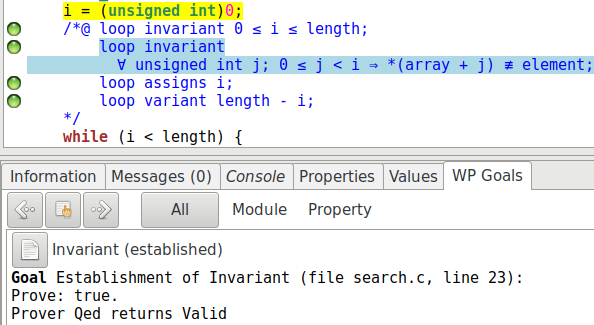
\includegraphics[scale=0.5]{3-4-trivial-establishment.png}
\caption{Trivial goal}
\label{fig:3-4-trivial}
\end{figure}

We note that this property, while quite complex, is proved easily proved
by Qed. If we look at the parts of the programs on which the proof
relies, we can see that the instruction \texttt{i\ =\ 0} is highlighted
and this is, indeed, the last instruction executed on \texttt{i} before
we start the loop. And consequently if we replace the value of
\texttt{i} by 0 inside the formula of the invariant, we get:

" For all j, greater or equal to 0 and strictly lower than 0 ``, this
part of the formula is necessarily false, our implication is then
necessarily true.

\subsection{Examples with mutable
arrays}\label{examples-with-mutable-arrays}

Let us present two examples with mutation of arrays. One with a mutation
of all memory locations, the other with selective modifications.

\subsubsection{Reset}\label{reset}

Let us have a look to the function that resets an array of integer to 0
(see Figure~\ref{fig:4-4-2-1-raz}).

\begin{figure}[htbp]
  \centering
\begin{footnotesize}\begin{Shaded}
\begin{Highlighting}[]
\CommentTok{#include <stddef.h>}

\CommentTok{/*@}
\CommentTok{  requires \textbackslash{}valid(array + (0 .. length-1));}
\CommentTok{  assigns  array[0 .. length-1];}
\CommentTok{  ensures  \textbackslash{}forall size_t i; 0 <= i < length ==> array[i] == 0;}
\CommentTok{*/}
\DataTypeTok{void} \NormalTok{raz(}\DataTypeTok{int}\NormalTok{* array, size_t length)\{}
  \CommentTok{/*@}
\CommentTok{    loop invariant 0 <= i <= length;}
\CommentTok{    loop invariant \textbackslash{}forall size_t j; 0 <= j < i ==> array[j] == 0;}
\CommentTok{    loop assigns i, array[0 .. length-1];}
\CommentTok{    loop variant length-i;}
\CommentTok{  */}
  \KeywordTok{for}\NormalTok{(size_t i = }\DecValTok{0}\NormalTok{; i < length; ++i)}
    \NormalTok{array[i] = }\DecValTok{0}\NormalTok{;}
\NormalTok{\}}
\end{Highlighting}
\end{Shaded}\end{footnotesize}
\caption{Function that resets an array}
\label{fig:4-4-2-1-raz}
\end{figure}

Let us just highlight the function and loop assign clauses. Again, we
can use the notation \texttt{n\ ..\ m} to indicate which parts of the
array are modified.

\subsubsection{Search and replace}\label{search-and-replace}

The last example we will detail to illustrate the proof of functions
with loops is the algorithm ``search and replace''. This algorithms will
selectively modify values in a range of memory locations. It is
generally harder to guide the tool in such a case, because on one hand
we must keep track of what is modified and what is not, and on the other
hand, the induction relies on this fact.

As an example, the first specification we can write for this function
could be the one illustrated by Figure~\ref{fig:4-4-2-2-sar}.

\begin{figure}[htbp]
  \centering
\begin{footnotesize}\begin{Shaded}
\begin{Highlighting}[]
\CommentTok{#include <stddef.h>}

\CommentTok{/*@}
\CommentTok{  requires \textbackslash{}valid(array + (0 .. length-1));}
\CommentTok{  assigns array[0 .. length-1];}

\CommentTok{  ensures \textbackslash{}forall size_t i; 0 <= i < length && \textbackslash{}old(array[i]) == old}
\CommentTok{             ==> array[i] == new;}
\CommentTok{  ensures \textbackslash{}forall size_t i; 0 <= i < length && \textbackslash{}old(array[i]) != old }
\CommentTok{             ==> array[i] == \textbackslash{}old(array[i]);}
\CommentTok{*/}
\DataTypeTok{void} \NormalTok{search_and_replace(}\DataTypeTok{int}\NormalTok{* array, size_t length, }\DataTypeTok{int} \NormalTok{old, }\DataTypeTok{int} \NormalTok{new)\{}
  \CommentTok{/*@}
\CommentTok{    loop invariant 0 <= i <= length;}
\CommentTok{    loop invariant \textbackslash{}forall size_t j; 0 <= j < i && \textbackslash{}at(array[j], Pre) == old }
\CommentTok{                     ==> array[j] == new;}
\CommentTok{    loop invariant \textbackslash{}forall size_t j; 0 <= j < i && \textbackslash{}at(array[j], Pre) != old }
\CommentTok{                     ==> array[j] == \textbackslash{}at(array[j], Pre);}
\CommentTok{    loop assigns i, array[0 .. length-1];}
\CommentTok{    loop variant length-i;}
\CommentTok{  */}
  \KeywordTok{for}\NormalTok{(size_t i = }\DecValTok{0}\NormalTok{; i < length; ++i)\{}
    \KeywordTok{if}\NormalTok{(array[i] == old) array[i] = new;}
  \NormalTok{\}}
\NormalTok{\}}
\end{Highlighting}
\end{Shaded}\end{footnotesize}
\caption{Specified search and replace function}
\label{fig:4-4-2-2-sar}
\end{figure}

We use the logic function '\at(v,
Label)\texttt{that\ gives\ us\ the\ value\ of\ the\ variable}v\texttt{at\ the\ program\ point}Label`.
If we look at the usage of this function here, we see that in the
invariant we try to establish a relation between the old values of the
array and the potentially new values:

\begin{footnotesize}\begin{Shaded}
\begin{Highlighting}[]
\CommentTok{/*@}
\CommentTok{  loop invariant \textbackslash{}forall size_t j; 0 <= j < i && \textbackslash{}at(array[j], Pre) == old }
\CommentTok{                   ==> array[j] == new;}
\CommentTok{  loop invariant \textbackslash{}forall size_t j; 0 <= j < i && \textbackslash{}at(array[j], Pre) != old }
\CommentTok{                   ==> array[j] == \textbackslash{}at(array[j], Pre);}
\CommentTok{*/}
\end{Highlighting}
\end{Shaded}\end{footnotesize}

For memory location, if it contained the value that must be replaced,
then it now contains the new value, else the value remains unchanged. In
fact, if we try to prove this invariant with WP, it fails. In such a
case, the simpler method is to add different assertions that will
express the different intermediate properties using assertions, that we
expect to be easily proved and that implies the invariant. Here, we can
easily notice that WP do not succeed in maintaining the knowledge that
we have not modified the end of the array yet:

\begin{footnotesize}\begin{Shaded}
\begin{Highlighting}[]
\KeywordTok{for}\NormalTok{(size_t i = }\DecValTok{0}\NormalTok{; i < length; ++i)\{}
    \CommentTok{//@assert array[i] == \textbackslash{}at(array[i], Pre); // proof failure}
    \KeywordTok{if}\NormalTok{(array[i] == old) array[i] = new;}
\NormalTok{\}}
\end{Highlighting}
\end{Shaded}\end{footnotesize}

We can add this information as an invariant:

\begin{footnotesize}\begin{Shaded}
\begin{Highlighting}[]
\CommentTok{/*@}
\CommentTok{  loop invariant 0 <= i <= length;}
\CommentTok{  loop invariant \textbackslash{}forall size_t j; 0 <= j < i && \textbackslash{}at(array[j], Pre) == old }
\CommentTok{                   ==> array[j] == new;}
\CommentTok{  loop invariant \textbackslash{}forall size_t j; 0 <= j < i && \textbackslash{}at(array[j], Pre) != old }
\CommentTok{                   ==> array[j] == \textbackslash{}at(array[j], Pre);}

\CommentTok{  // The end of the array remains the same:}
\CommentTok{  loop invariant \textbackslash{}forall size_t j; i <= j < length}
\CommentTok{                     ==> array[j] == \textbackslash{}at(array[j], Pre);}
\CommentTok{  loop assigns i, array[0 .. length-1];}
\CommentTok{  loop variant length-i;}
\CommentTok{*/}
\KeywordTok{for}\NormalTok{(size_t i = }\DecValTok{0}\NormalTok{; i < length; ++i)\{}
  \KeywordTok{if}\NormalTok{(array[i] == old) array[i] = new;}
\NormalTok{\}}
\end{Highlighting}
\end{Shaded}\end{footnotesize}

And this time the proof will succeed. Note that if we try to prove this
invariant directly with the verification of the absence of RTE, Alt-Ergo
may not succeed (CVC4 succeeds without problem). In this case, we can
launch these proofs separately (first without, and then with the absence
of RTE checking) or else add assertions that allows to guide the proof
inside the loop:

\begin{footnotesize}\begin{Shaded}
\begin{Highlighting}[]
\KeywordTok{for}\NormalTok{(size_t i = }\DecValTok{0}\NormalTok{; i < length; ++i)\{}
  \KeywordTok{if}\NormalTok{(array[i] == old) array[i] = new;}

  \CommentTok{/*@ assert \textbackslash{}forall size_t j; i < j < length }
\CommentTok{               ==> array[j] == \textbackslash{}at(array[j], Pre);                      */}
  \CommentTok{/*@ assert \textbackslash{}forall size_t j; 0 <= j <= i && \textbackslash{}at(array[j], Pre) == old }
\CommentTok{               ==> array[j] == new;                                     */}
  \CommentTok{/*@ assert \textbackslash{}forall size_t j; 0 <= j <= i && \textbackslash{}at(array[j], Pre) != old }
\CommentTok{               ==> array[j] == \textbackslash{}at(array[j], Pre);                      */}    
\NormalTok{\}}
\end{Highlighting}
\end{Shaded}\end{footnotesize}

As we will try to prove more complex properties, particularly when
programs involve loops, there will be a part of ``trial and error'' in
order to understand what the provers miss to establish the proof.

It can miss hypotheses. In this case, we can try to add assertions to
guide the prover. With some experience, we can read the content of the
proof obligations or try to perform the proof with the Coq interactive
prover to see whether the proof seems to be possible. Sometimes, the
prover just need more time, in such a case, we can (sometimes a lot)
augment the timeout value. Of course, the property can be too hard for
the prover, and in this case, we will have to write the proof ourselves
with an interactive prover.

Finally, the implementation can be indeed incorrect, and in this case we
have to fix it. Here, we will use test and not proof, because a test
allows us to prove the presence of a bug and to analyze this bug.

Dans cette partie nous avons pu voir comment se traduisent les
affectations et les structures de contrôle d'un point de vue logique.
Nous nous sommes beaucoup attardés sur les boucles parce que c'est là
que se trouvent la majorité des difficultés lorsque nous voulons
spécifier et prouver un programme par vérification déductive, les
annotations ACSL qui leur sont spécifiques nous permettent d'exprimer le
plus précisément possible leur comportement.

Pour la suite, nous allons nous attarder plus précisément sur les
constructions que nous offre le langage ACSL du côté de la logique.
Elles sont très importantes parce que ce sont elles qui vont nous
permettre de nous abstraire du code pour avoir des spécifications plus
compréhensibles et plus aisément prouvables.

\chapter{ACSL - Properties}\label{acsl---properties}

From the beginning of this tutorial, we have used different predicates
and logic functions provided by ACSL : \texttt{\textbackslash{}valid},
\texttt{\textbackslash{}valid\_read},
\texttt{\textbackslash{}separated}, \texttt{\textbackslash{}old} and
\texttt{at}. There are others built-in predicates but we will not
present them all, the reader can refer to
\href{http://frama-c.com/download.html}{the documentation (ACSL
implementation)} (note that everything is not necessarily supported by
WP).

ACSL allows us to do something more than ``just'' specify our code using
existing predicates and functions. We can define our own predicates,
functions, relations, etc. Doing this, we can have more abstract
specifications. It also allows us to factor specifications (for example
defining what is a valid array), which have two pleasant consequences:
our specifications are more readable and more understandable, and we can
reuse existing proofs to ease the proof of new programs.

\section{Some logical types}\label{some-logical-types}

ACSL provides two types that will allow us to write properties or
functions without having to take about constraints due to the size of
the representation of primitive C types in memory. These types are
\texttt{integer} and \texttt{real}, which respectively represent
mathematical integers and reals (that are modeled to be as near the
reality we can, but this notion cannot be perfectly handled).

From now, we will often use integers instead of classical C
\texttt{int}s. The reason is simply that a lot of properties and
definitions are true regardless the size of the machine integer we have
in input.

On the other hand, we will not talk about the differences that exists
between \texttt{real} and \texttt{float/double}. It would require to
speak about precise numerical calculus, and about proofs of programs
that rely on such calculus which could deserve an entire dedicated
tutorial.

\section{Predicates}\label{predicates}

A predicate is a property about different objects that can be true or
false. To sum up, we are writing predicates from the beginning of this
tutorial in precondition, postcondition, assertion and loop invariant.
ACSL allows us to name these predicates, as we could do for a boolean
function in C, for example. An important difference, however, is that
predicates (as well as functions that we will see later) must be pure,
they cannot produce side effects by modifying a pointed value for
example.

These predicates can receive some parameters. Moreover, they can also
receive some C labels that will allow us to establish relations between
different program points.

\subsection{Syntax}\label{syntax}

Predicates are introduced using ACSL annotations. The syntax is the
following:

\begin{footnotesize}\begin{Shaded}
\begin{Highlighting}[]
\CommentTok{/*@}
\CommentTok{  predicate named_predicate \{Lbl0, Lbl1, ..., LblN\}(type0 arg0, type1 arg1, ..., typeN argN) =}
\CommentTok{    //a logic relations between all these things}
\CommentTok{*/}
\end{Highlighting}
\end{Shaded}\end{footnotesize}

For example, we can define the predicate that checks whether an integer
in memory is changed between to particular program points:

\begin{footnotesize}\begin{Shaded}
\begin{Highlighting}[]
\CommentTok{/*@}
\CommentTok{  predicate unchanged\{L0, L1\}(int* i) =}
\CommentTok{    \textbackslash{}at(*i, L0) == \textbackslash{}at(*i, L1);}
\CommentTok{*/}
\end{Highlighting}
\end{Shaded}\end{footnotesize}

\begin{zdsalertblock}{Warning}
  Keep in mind that passing a value to a predicate is done, as it is done in C,
  by value. We cannot write this predicate by directly passing \texttt{i} in
  parameter:
  \begin{footnotesize}\begin{Shaded}
      \begin{Highlighting}[]
\CommentTokAlt{/*@}
\CommentTokAlt{  predicate unchanged\{L0, L1\}(int i) =}
\CommentTokAlt{    \textbackslash{}at(i, L0) == \textbackslash{}at(i, L1);}
\CommentTokAlt{*/}
      \end{Highlighting}
  \end{Shaded}\end{footnotesize}
  Since \texttt{i} is just a copy of the received variable.
\end{zdsalertblock}
  
We can verify this code using our predicate:

\begin{footnotesize}\begin{Shaded}
\begin{Highlighting}[]
\DataTypeTok{int} \NormalTok{main()\{}
  \DataTypeTok{int} \NormalTok{i = }\DecValTok{13}\NormalTok{;}
  \DataTypeTok{int} \NormalTok{j = }\DecValTok{37}\NormalTok{;}

 \NormalTok{Begin:}
  \NormalTok{i = }\DecValTok{23}\NormalTok{;}
 
  \CommentTok{//@assert ! unchanged\{Begin, Here\}(&i);}
  \CommentTok{//@assert   unchanged\{Begin, Here\}(&j);}
\NormalTok{\}}
\end{Highlighting}
\end{Shaded}\end{footnotesize}

We can also have a look to the goals generated by WP and notice that,
even it is slightly (syntactically) modified, the predicate is not
unrolled by WP. The provers will determine if they need to use the
definition of the predicate.

As we said earlier, one important use of predicates (and logic
functions) is to make our specifications more readable and to factor it.
An example can be to write a predicate that expresses the validity of an
array in read or write. It allows us to avoid writing the complete
expression every time we need it and to make it readable quickly:

\begin{footnotesize}\begin{Shaded}
\begin{Highlighting}[]
\CommentTok{/*@}
\CommentTok{  predicate valid_range_rw(int* t, integer n) =}
\CommentTok{    n >= 0 && \textbackslash{}valid(t + (0 .. n-1));}
\CommentTok{  predicate valid_range_ro(int* t, integer n) =}
\CommentTok{    n >= 0 && \textbackslash{}valid_read(t + (0 .. n-1));}
\CommentTok{*/}
\CommentTok{/*@}
\CommentTok{  requires 0 < length;}
\CommentTok{  requires valid_range_ro(array, length);}
\CommentTok{  //...}
\CommentTok{*/}
\DataTypeTok{int}\NormalTok{* search(}\DataTypeTok{int}\NormalTok{* array, size_t length, }\DataTypeTok{int} \NormalTok{element)}
\end{Highlighting}
\end{Shaded}\end{footnotesize}

In these specification, we do not give an explicit label to predicates
for their definition, nor for their use. For the definition, Frama-C
automatically creates an implicit label. At predicate use, the given
label is implicitly \texttt{Here}. The fact we do not explicitly define
the label in the definition of a predicate does not forbid to explicitly
give a label when we use it.

Of course, predicates can be defined in header files in order to produce
an utility library for specification for example.

\subsection{Abstraction}\label{abstraction}

An other important use of predicates is to define the logical state of
our data structures when programs start to be more complex. Our data
structures must usually respect an invariant (again) that each
manipulation function must maintain in order to ensure that the data
structure will always remain coherent and usable through future calls.

It allows us to ease the reading of specifications. For example, we can
define the specification required to ensure the safety of a fixed size
stack. It could be done as illustrated there:

\begin{footnotesize}\begin{Shaded}
\begin{Highlighting}[]
\KeywordTok{struct} \NormalTok{stack_int\{}
  \NormalTok{size_t top;}
  \DataTypeTok{int}    \NormalTok{data[MAX_SIZE];}
\NormalTok{\};}

\CommentTok{/*@}
\CommentTok{  predicate valid_stack_int(struct stack_int* s) = // to be defined ;}
\CommentTok{  predicate empty_stack_int(struct stack_int* s) = // to be defined ;}
\CommentTok{  predicate full_stack_int(struct stack_int* s) =  // to be defined ;}
\CommentTok{*/}

\CommentTok{/*@}
\CommentTok{  requires \textbackslash{}valid(s);}
\CommentTok{  assigns *s;}
\CommentTok{  ensures valid_stack_int(s) && empty_stack_int(s);}
\CommentTok{*/}
\DataTypeTok{void} \NormalTok{initialize(}\KeywordTok{struct} \NormalTok{stack_int* s);}

\CommentTok{/*@}
\CommentTok{  requires valid_stack_int(s) && !full_stack_int(s);}
\CommentTok{  assigns  *s;}
\CommentTok{  ensures valid_stack_int(s);}
\CommentTok{*/}
\DataTypeTok{void} \NormalTok{push(}\KeywordTok{struct} \NormalTok{stack_int* s, }\DataTypeTok{int} \NormalTok{value);}

\CommentTok{/*@}
\CommentTok{  requires valid_stack_int(s) && !empty_stack_int(s);}
\CommentTok{  assigns \textbackslash{}nothing;}
\CommentTok{*/}
\DataTypeTok{int}  \NormalTok{top(}\KeywordTok{struct} \NormalTok{stack_int* s);}

\CommentTok{/*@}
\CommentTok{  requires valid_stack_int(s) && !empty_stack_int(s);}
\CommentTok{  assigns *s;}
\CommentTok{  ensures valid_stack_int(s);}
\CommentTok{*/}
\DataTypeTok{void} \NormalTok{pop(}\KeywordTok{struct} \NormalTok{stack_int* s);}

\CommentTok{/*@}
\CommentTok{  requires valid_stack_int(s);}
\CommentTok{  assigns \textbackslash{}nothing;}
\CommentTok{  ensures \textbackslash{}result == 1 <==> empty_stack_int(s);}
\CommentTok{*/}
\DataTypeTok{int}  \NormalTok{is_empty(stack_int_t s);}


\CommentTok{/*@}
\CommentTok{  requires valid_stack_int(s);}
\CommentTok{  assigns \textbackslash{}nothing;}
\CommentTok{  ensures \textbackslash{}result == 1 <==> full_stack_int(s);}
\CommentTok{*/}
\DataTypeTok{int}  \NormalTok{is_full(stack_int_t s);}
\end{Highlighting}
\end{Shaded}\end{footnotesize}

Here, the specification does not express functional properties. For
example, we do not specify that when we perform the push of a value, and
then we ask for the top of the stack, we get the same value. But we
already have enough details to ensure that, even if we cannot prove that
we always get the right result (behaviors such as ``if I push \(v\), top
returns \(v\)''), we can still guarantee that we do not produce runtime
errors (if we provide correct predicates for the stack, and to prove
that the implementation of our functions ensures that no runtime error
can occur).

\section{Logic functions}\label{logic-functions}

Logic functions are meant to describe functions that can only be used in
specifications. It allows us, first, to factor those specifications and,
second, to define some operations on \texttt{integer} or \texttt{real}
with the guarantee that they cannot overflow since they are mathematical
types.

Like predicates, they can receive different labels and values in
parameter.

\subsection{Syntax}\label{syntax-1}

To define a logic function, the syntax is the following:

\begin{footnotesize}\begin{Shaded}
\begin{Highlighting}[]
\CommentTok{/*@}
\CommentTok{  logic return_type my_function\{ Label0, ..., LabelN \}( type0 arg0, ..., typeN argN ) =}
\CommentTok{    formula using the arguments ;}
\CommentTok{*/}
\end{Highlighting}
\end{Shaded}\end{footnotesize}

We can for example define a mathematical
\href{https://en.wikipedia.org/wiki/Linear_function_(calculus)}{linear
function} using a logic function:

\begin{footnotesize}\begin{Shaded}
\begin{Highlighting}[]
\CommentTok{/*@}
\CommentTok{  logic integer ax_b(integer a, integer x, integer b) =}
\CommentTok{    a * x + b;}
\CommentTok{*/}
\end{Highlighting}
\end{Shaded}\end{footnotesize}

And it can be used to prove the source code of the following function:

\begin{footnotesize}\begin{Shaded}
\begin{Highlighting}[]
\CommentTok{/*@ }
\CommentTok{  assigns \textbackslash{}nothing ;}
\CommentTok{  ensures \textbackslash{}result == ax_b(3,x,4); }
\CommentTok{*/}
\DataTypeTok{int} \NormalTok{function(}\DataTypeTok{int} \NormalTok{x)\{}
  \KeywordTok{return} \DecValTok{3}\NormalTok{*x + }\DecValTok{4}\NormalTok{;}
\NormalTok{\}}
\end{Highlighting}
\end{Shaded}\end{footnotesize}

\begin{figure}[htbp]
\centering
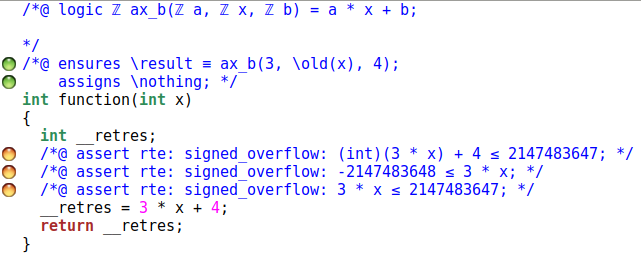
\includegraphics[scale=0.5]{4-3-affine-1.png}
\caption{Some overflows seem to be possible}
\label{fig:4-3-affine-1}
\end{figure}

This code is indeed proved but some runtime-errors seems to be possible
(see Figure~\ref{fig:4-3-affine-1}).
We can again define some mathematical logic function, that will, from a
logic point of view, provide the bounds of the affine function according
to the machine type we use? It allows us to then add our bound checking
in preconditon or the function.

\begin{footnotesize}\begin{Shaded}
\begin{Highlighting}[]
\CommentTok{/*@}
\CommentTok{  logic integer limit_int_min_ax_b(integer a, integer b) =}
\CommentTok{    (a == 0) ? (b > 0) ? INT_MIN : INT_MIN-b :}
\CommentTok{    (a <  0) ? (INT_MAX-b)/a :}
\CommentTok{               (INT_MIN-b)/a ;}

\CommentTok{  logic integer limit_int_max_ax_b(integer a, integer b) =}
\CommentTok{    (a == 0) ? (b > 0) ? INT_MAX-b : INT_MAX :}
\CommentTok{    (a <  0) ? (INT_MIN-b)/a :}
\CommentTok{               (INT_MAX-b)/a ;}
\CommentTok{*/}

\CommentTok{/*@}
\CommentTok{  requires limit_int_min_ax_b(3,4) < x < limit_int_max_ax_b(3,4);}
\CommentTok{  assigns \textbackslash{}nothing ;}
\CommentTok{  ensures \textbackslash{}result == ax_b(3,x,4);}
\CommentTok{*/}
\DataTypeTok{int} \NormalTok{function(}\DataTypeTok{int} \NormalTok{x)\{}
  \KeywordTok{return} \DecValTok{3}\NormalTok{*x + }\DecValTok{4}\NormalTok{;}
\NormalTok{\}}
\end{Highlighting}
\end{Shaded}\end{footnotesize}

\begin{zdsblock}
  Note that, as in specifications, computations are done using mathematical
  integers, we then do not need to care about some overflow risk with the
  computation or \texttt{INT\_MIN-b} or \texttt{INT\_MAX-b}.
\end{zdsblock}
  
Once this specification is provided, everything is fine. Of course, we
could provide manually these bounds every time we create an linear logic
function. But, by creating these bound computation function, we directly
get a way to compute them automatically which is quite comfortable.

\subsection{Recursive functions and limits of logic
functions}\label{recursive-functions-and-limits-of-logic-functions}

Logic functions (as well as predicates) can be recursively defined.
However, such an approach will rapidly show some limits in their use for
program proof. Indeed, when automatic solver will reason on such logic
properties, if such a function is met, it will be necessary to evaluate
it, and SMT solvers are not meant to be efficient for this task, which
will be generally costly, producing to long proof resolution and
eventually timeouts.

We can have a concrete example with the factorial function, using logic
and using C language:

\begin{footnotesize}\begin{Shaded}
\begin{Highlighting}[]
\CommentTok{/*@}
\CommentTok{  logic integer factorial(integer n) = (n <= 0) ? 1 : n * factorial(n-1);}
\CommentTok{*/}

\CommentTok{/*@ }
\CommentTok{  assigns \textbackslash{}nothing ;}
\CommentTok{  ensures \textbackslash{}result == factorial(n) ; }
\CommentTok{*/}
\DataTypeTok{unsigned} \NormalTok{facto(}\DataTypeTok{unsigned} \NormalTok{n)\{}
  \KeywordTok{return} \NormalTok{(n == }\DecValTok{0}\NormalTok{) ? }\DecValTok{1} \NormalTok{: n * facto(n}\DecValTok{-1}\NormalTok{);}
\NormalTok{\}}
\end{Highlighting}
\end{Shaded}\end{footnotesize}

Without checking overflows, this function is easy and fast to prove. If
we add runtime error checking, RTE does not add any assertion to check
the absence of overflow on unsigned integers, since it is specified by
the C norm (and is then a defined behavior). If we want to add an
assertion at this point, we can ask WP to generate its own bound
checking by right-clicking on the function and then asking ``insert
WP-safety guards''. And in this case, an overflow is not proved to be
absent.

On \texttt{unsigned}, the maximum value for which we can compute
factorial is 12. If we go further, it overflows. We can then add this
preconditon:

\begin{footnotesize}\begin{Shaded}
\begin{Highlighting}[]
\CommentTok{/*@ }
\CommentTok{  requires n <= 12 ;}
\CommentTok{  assigns \textbackslash{}nothing ;}
\CommentTok{  ensures \textbackslash{}result == factorial(n) ; }
\CommentTok{*/}
\DataTypeTok{unsigned} \NormalTok{facto(}\DataTypeTok{unsigned} \NormalTok{n)\{}
  \KeywordTok{return} \NormalTok{(n == }\DecValTok{0}\NormalTok{) ? }\DecValTok{1} \NormalTok{: n * facto(n}\DecValTok{-1}\NormalTok{);}
\NormalTok{\}}
\end{Highlighting}
\end{Shaded}\end{footnotesize}

If we ask for a proof on this input, Alt-ergo will probably fail,
whereas Z3 can compute the proof in less than a second. The reason is
that in this case, the heuristics that are used by Z3 consider that it
is a good idea to spend a bit more of time on the evaluation of the
function. We can for example change the maximum value of \texttt{n} to
see how the different provers behave. With a \texttt{n} fixed to 9,
Alt-ergo produces a proof in less than 10 seconds, whereas with a value
of 10, even a minute is not enough.

Logic functions can then be defined recursively but without some more
help, we are rapidly limited by the fact that provers will need to
perform evaluation or to ``reason'' by induction, two tasks for which
they are not efficient, which will limit our possibility for program
proofs.

\section{Lemmas}\label{lemmas}

Lemmas are general properties about predicates or functions. Once these
properties are expressed, their proof can be performed (one time) and
the provers will then be able to use this result to perform other proofs
without requiring to perform again all steps needed to perform the
original proof if it appears in a much longer proof about an other
property.

For example, lemmas allow us to express properties about recursive
functions in order to get easier proofs when we are interested in
proving properties that use such functions.

\subsection{Syntax}\label{syntax-2}

Again, we introduce lemmas using ACSL annotations. The syntax is
following:

\begin{footnotesize}\begin{Shaded}
\begin{Highlighting}[]
\CommentTok{/*@}
\CommentTok{  lemma name_of_the_lemma \{ Label0, ..., LabelN \}:}
\CommentTok{    property ;}
\CommentTok{*/}
\end{Highlighting}
\end{Shaded}\end{footnotesize}

This time, the properties we want to express do not depend on received
parameters (except for labels). So we will express these properties on
universally quantified variables. For example, we can state this lemma,
which is true, even if it is trivial:

\begin{footnotesize}\begin{Shaded}
\begin{Highlighting}[]
\CommentTok{/*@}
\CommentTok{  lemma lt_plus_lt:}
\CommentTok{    \textbackslash{}forall integer i, j ; i < j ==> i+1 < j+1;}
\CommentTok{*/}
\end{Highlighting}
\end{Shaded}\end{footnotesize}

This proof can be performed using WP. The property is, of course, proved
using only Qed.

\subsection{Example: properties about linear
functions}\label{example-properties-about-linear-functions}

We can come back to our linear functions and express some interesting
properties about them:

\begin{footnotesize}\begin{Shaded}
\begin{Highlighting}[]
\CommentTok{/* @}
\CommentTok{  lemma ax_b_monotonic_neg:}
\CommentTok{    \textbackslash{}forall integer a, b, i, j ;}
\CommentTok{      a <  0 ==> i <= j ==> ax_b(a, i, b) >= ax_b(a, j, b);}
\CommentTok{  lemma ax_b_monotonic_pos:}
\CommentTok{    \textbackslash{}forall integer a, b, i, j ;}
\CommentTok{      a >  0 ==> i <= j ==> ax_b(a, i, b) <= ax_b(a, j, b);}
\CommentTok{  lemma ax_b_monotonic_nul:}
\CommentTok{    \textbackslash{}forall integer a, b, i, j ;}
\CommentTok{      a == 0 ==> ax_b(a, i, b) == ax_b(a, j, b);}
\CommentTok{*/}
\end{Highlighting}
\end{Shaded}\end{footnotesize}

For these proofs, Alt-ergo, will probably not be able to discharge
generated goals. In this case, Z3 will certainly perform it. We can then
write some code examples:

\begin{footnotesize}\begin{Shaded}
\begin{Highlighting}[]
\CommentTok{/*@}
\CommentTok{  requires a > 0;}
\CommentTok{  requires limit_int_min_ax_b(a,4) < x < limit_int_max_ax_b(a,4);}
\CommentTok{  assigns \textbackslash{}nothing ;}
\CommentTok{  ensures \textbackslash{}result == ax_b(a,x,4);}
\CommentTok{*/}
\DataTypeTok{int} \NormalTok{function(}\DataTypeTok{int} \NormalTok{a, }\DataTypeTok{int} \NormalTok{x)\{}
  \KeywordTok{return} \NormalTok{a*x + }\DecValTok{4}\NormalTok{;}
\NormalTok{\}}

\CommentTok{/*@ }
\CommentTok{  requires a > 0;}
\CommentTok{  requires limit_int_min_ax_b(a,4) < x < limit_int_max_ax_b(a,4) ;}
\CommentTok{  requires limit_int_min_ax_b(a,4) < y < limit_int_max_ax_b(a,4) ;}
\CommentTok{  assigns \textbackslash{}nothing ;}
\CommentTok{*/}
\DataTypeTok{void} \NormalTok{foo(}\DataTypeTok{int} \NormalTok{a, }\DataTypeTok{int} \NormalTok{x, }\DataTypeTok{int} \NormalTok{y)\{}
  \DataTypeTok{int} \NormalTok{fmin, fmax;}
  \KeywordTok{if}\NormalTok{(x < y)\{}
    \NormalTok{fmin = function(a,x);}
    \NormalTok{fmax = function(a,y);}
  \NormalTok{\} }\KeywordTok{else} \NormalTok{\{}
    \NormalTok{fmin = function(a,y);}
    \NormalTok{fmax = function(a,x);}
  \NormalTok{\}}
  \CommentTok{//@assert fmin <= fmax;}
\NormalTok{\}}
\end{Highlighting}
\end{Shaded}\end{footnotesize}

If we do not give the lemmas provided earlier, Alt-ergo will not be able
to prove the proof that \texttt{fmin} is lesser or equal to
\texttt{fmax}. With the lemmas it is however very easy for it since the
property is the simply an instance of the lemma
\texttt{ax\_monotonic\_pos}, the proof is then trivial as our lemma is
considered to be true when are not currently proving it.

In this part of the tutorial, we have seen different ACSL construct that
allow us to factor our specifications and to express general properties
that can be used by our solver to easy their work.

All techniques we have talk about are safe, since they do not \emph{a
priori} allow us to write false or contradictory specifications. At
least if the specification only use such logic constructions and if
every lemma, precondition (at call site), every postcondition,
assertion, variant and invariant is correctly proved, the code is
correct.

However, sometimes, such constructions are not enough to express all
properties we want to express about our programs. The next constructions
we will see give us some new possibilities about it, but it will be
necessary to be really careful using them since an error would allow us
to introduction false assumptions or silently modify the program we are
verifying.

\chapter{ACSL - Logic definitions and
code}\label{acsl---logic-definitions-and-code}

In this part of the tutorial, we will present two important notions of
ACSL:

\begin{itemize}
\tightlist
\item
  axiomatic definitions,
\item
  ghost code.
\end{itemize}

In some cases, this two notions are absolutely needed to ease the
process of specification and, more importantly, proof. On one hand by
forcing some properties to be more abstract when an explicit modeling
involve to much computation during proof, on the other hand by forcing
some properties to be explicitly modeled since they are harder to reason
with when they are implicit.

Using this two notions, we expose ourselves to the possibility to make
our proof irrelevant if we make mistakes writing specification with it.
The first one allows us to introduce ``false'' in our assumptions, or to
write imprecise definitions. The second one opens the risk to silently
modify the verified program \ldots{} making us prove another program,
which is not the one we want to prove.

\section{Axiomatic definitions}\label{axiomatic-definitions}

Axioms are properties we state to be true no matter the situation. It is
a good way to state complex properties that will allow the proof process
to be more efficient by abstracting their complexity. Of course, as any
property expressed as an axiom is assumed to be true, we have to be very
careful when we use them to defined properties: if we introduce a false
property in our assumptions, ``false'' becomes ``true'' and we can then
prove anything.

\subsection{Syntax}\label{syntax-3}

Axiomatic definitions are introduced using this syntax:

\begin{footnotesize}\begin{Shaded}
\begin{Highlighting}[]
\CommentTok{/*@}
\CommentTok{  axiomatic Name_of_the_axiomatic_definition \{}
\CommentTok{    // here we can define or declare functions and predicates}

\CommentTok{    axiom axiom_name \{ Label0, ..., LabelN \}:}
\CommentTok{      // property ;}

\CommentTok{    axiom other_axiom_name \{ Label0, ..., LabelM \}:}
\CommentTok{      // property ;}

\CommentTok{    // ... we can put as many axioms we need}
\CommentTok{  \}}
\CommentTok{*/}
\end{Highlighting}
\end{Shaded}\end{footnotesize}

\clearpage
For example, we can write this axiomatic block:

\begin{footnotesize}\begin{Shaded}
\begin{Highlighting}[]
\CommentTok{/*@}
\CommentTok{  axiomatic lt_plus_lt\{}
\CommentTok{    axiom always_true_lt_plus_lt:}
\CommentTok{      \textbackslash{}forall integer i, j; i < j ==> i+1 < j+1 ;}
\CommentTok{  \}}
\CommentTok{*/}
\end{Highlighting}
\end{Shaded}\end{footnotesize}

And we can see that in Frama-C, this property is actually assumed to be
true (see Figure~\ref{fig:5-1-1-fst-axiom}).

\begin{figure}[htbp]
\centering
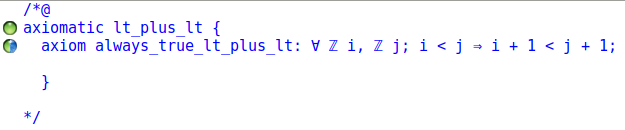
\includegraphics[scale=0.5]{5-1-1-premier-axiome.png}
\caption{First axiom, assumed to be true by Frama-C}
\label{fig:5-1-1-fst-axiom}
\end{figure}

\begin{zdssecretblock}{Off topic}
  Currently, our automatic solvers are not
  powerful enough to compute \emph{the Answer to the Ultimate
Question of Life, the Universe, and Everything}. We can help
them by stating it as an axiom! Now, we just have to 
understand the question to determine in which case this result can be
useful \ldots{}
  \begin{footnotesize}\begin{Shaded}
\begin{Highlighting}[]
\CommentTokAlt{/*@}
\CommentTokAlt{  axiomatic Ax_answer_to_the_ultimate_question_of_life_the_universe_and_everything \{}
\CommentTokAlt{    logic integer the_ultimate_question_of_life_the_universe_and_everything\{L\} ;}
\CommentTokAlt{}
\CommentTokAlt{    axiom answer\{L\}:}
\CommentTokAlt{      the_ultimate_question_of_life_the_universe_and_everything\{L\} = 42;}
\CommentTokAlt{}
\CommentTokAlt{*/}
\end{Highlighting}
    \end{Shaded}\end{footnotesize}
\end{zdssecretblock}

\subsubsection{Link with lemmas}\label{link-with-lemmas}

Lemmas and axioms allows to express the same types of properties.
Namely, properties expressed about quantified variables (and possibly
global variables, but it is quite rare since it is often difficult to
find a global property about such variables being both true and
interesting). Apart this first common point, we can also notice that
when we are not considering the definition of the lemma itself, lemmas
are assumed to be true by WP exactly as axioms are.

The only difference between lemmas and axioms from a proof point of view
is that we must provide a proof that each lemma is true, whereas an
axiom is always assumed to be true.

\subsection{Recursive function or predicate
definitions}\label{recursive-function-or-predicate-definitions}

Axiomatic definition of recursive functions and predicates are
particularly useful since they will prevent provers to unroll the
recursion when is is possible.

The idea is then not to define directly the function or the predicate
but to declare it and then to define axioms that will specify its
behavior. If we come back to the factorial function, we can define it
axiomatically as follows:

\begin{footnotesize}\begin{Shaded}
\begin{Highlighting}[]
\CommentTok{/*@}
\CommentTok{  axiomatic Factorial\{}
\CommentTok{    logic integer factorial(integer n);}
\CommentTok{    }
\CommentTok{    axiom factorial_0:}
\CommentTok{      \textbackslash{}forall integer i; i <= 0 ==> 1 == factorial(i) ;}

\CommentTok{    axiom factorial_n:}
\CommentTok{      \textbackslash{}forall integer i; i > 0 ==> i * factorial(i-1) == factorial(i) ;}
\CommentTok{  \}}
\CommentTok{*/}
\end{Highlighting}
\end{Shaded}\end{footnotesize}

In this axiomatic definition, our function do not have a body. Its
behavior is only defined by the axioms we have stated about it.

A small subtlety is that we must take care about the fact that if some
axioms state properties about the content of some pointed memory cells,
we have to specify considered memory blocks using the \texttt{reads}
notation in the declaration. If we omit such a specification, the
predicate or function will be considered to be stated about the received
pointers and not about pointer memory blocks. So, if the code modifies
the content of an array for which we had proven that the predicate or
function give some result, this result will not be considered to be
potentially different.

If, for example, we want to define that an array only contains 0s, we
have to write it as follows:

\begin{footnotesize}\begin{Shaded}
\begin{Highlighting}[]
\CommentTok{/*@}
\CommentTok{  axiomatic A_all_zeros\{}
\CommentTok{    predicate zeroed\{L\}(int* a, integer b, integer e) reads a[b .. e-1];}

\CommentTok{    axiom zeroed_empty\{L\}:}
\CommentTok{      \textbackslash{}forall int* a, integer b, e; b >= e ==> zeroed\{L\}(a,b,e);}

\CommentTok{    axiom zeroed_range\{L\}:}
\CommentTok{      \textbackslash{}forall int* a, integer b, e; b < e ==>}
\CommentTok{        zeroed\{L\}(a,b,e-1) && a[e-1] == 0 <==> zeroed\{L\}(a,b,e);}
\CommentTok{  \}}
\CommentTok{*/}
\end{Highlighting}
\end{Shaded}\end{footnotesize}

And we can again prove that our reset to 0 is correct with this new
definition:

\begin{footnotesize}\begin{Shaded}
\begin{Highlighting}[]
\ErrorTok{#include <stddef.h>}

\CommentTok{/*@}
\CommentTok{  requires \textbackslash{}valid(array + (0 .. length-1));}
\CommentTok{  assigns  array[0 .. length-1];}
\CommentTok{  ensures  zeroed(array,0,length);}
\CommentTok{*/}
\DataTypeTok{void} \NormalTok{reset(}\DataTypeTok{int}\NormalTok{* array, size_t length)\{}
  \CommentTok{/*@}
\CommentTok{    loop invariant 0 <= i <= length;}
\CommentTok{    loop invariant zeroed(array,0,i);}
\CommentTok{    loop assigns i, array[0 .. length-1];}
\CommentTok{    loop variant length-i;}
\CommentTok{  */}
  \KeywordTok{for}\NormalTok{(size_t i = }\DecValTok{0}\NormalTok{; i < length; ++i)}
    \NormalTok{array[i] = }\DecValTok{0}\NormalTok{;}
\NormalTok{\}}
\end{Highlighting}
\end{Shaded}\end{footnotesize}

Depending on the Frama-C or automatic solvers versions, the proof of the
preservation of the invariant could fail. A reason to this fail is the
fact that the prover forget that cells preceding the one we are
currently processing are actually still set to 0. We can add a lemma in
our knowledge base, stating that if a set of values of an array did not
change between two program points, the first one being a point where the
property ``zeroed'' is verified, then the property is still verified at
the second program point.

\begin{footnotesize}\begin{Shaded}
\begin{Highlighting}[]
\CommentTok{/*@}
\CommentTok{  predicate same_elems\{L1,L2\}(int* a, integer b, integer e) =}
\CommentTok{    \textbackslash{}forall integer i; b <= i < e ==> \textbackslash{}at(a[i],L1) == \textbackslash{}at(a[i],L2);}

\CommentTok{  lemma no_changes\{L1,L2\}:}
\CommentTok{    \textbackslash{}forall int* a, integer b, e;}
\CommentTok{      same_elems\{L1,L2\}(a,b,e) ==> zeroed\{L1\}(a,b,e) ==> zeroed\{L2\}(a,b,e);}
\CommentTok{*/}
\end{Highlighting}
\end{Shaded}\end{footnotesize}

Then we can add an assertion to specify what did not change between the
beginning of the loop block (pointed by the label \texttt{L} in the
code) and the end (which is \texttt{Here} since we state the property at
the end):

\begin{footnotesize}\begin{Shaded}
\begin{Highlighting}[]
\KeywordTok{for}\NormalTok{(size_t i = }\DecValTok{0}\NormalTok{; i < length; ++i)\{}
  \NormalTok{L:}
  \NormalTok{array[i] = }\DecValTok{0}\NormalTok{;}
  \CommentTok{//@ assert same_elems\{L,Here\}(array,0,i);}
\NormalTok{\}}
\end{Highlighting}
\end{Shaded}\end{footnotesize}

Note that in this new version of the code, the property stated by our
lemma is not proved using automatic solver, that cannot reason by
induction. If the reader is curious, the (quite simple) Coq proof can be
found there:

\begin{zdssecretblock}{Preuve Coq}
  \begin{footnotesize}
  \begin{footnotesize}\begin{Shaded}
\begin{Highlighting}[]
(* Generated par WP *)
Definition P_same_elems (Mint_0 : farray addr Z) (Mint_1 : farray addr Z)
    (a : addr) (b : Z) (e : Z) : Prop :=
    forall (i : Z), let a_1 := (shift_sint32 a i%Z) in ((b <= i)%Z) ->
      ((i < e)%Z) -> (((Mint_0.[ a_1 ]) = (Mint_1.[ a_1 ]))%Z).
Goal
  forall (i_1 i : Z), forall (t_1 t : farray addr Z), forall (a : addr),
  ((P_zeroed t a i_1%Z i%Z)) ->
    ((P_same_elems t_1 t a i_1%Z i%Z)) ->
      ((P_zeroed t_1 a i_1%Z i%Z)).
(* Our proof *)
Proof.
  intros b e.
  (* By induction on the distance between b and e *)
  induction e using Z_induction with (m := b) ; intros mem_l2 mem_l1 a Hz_l1 Hsame.
  (* Base case: "empty" axiom *)
  + apply A_A_all_zeros.Q_zeroed_empty ; assumption.
  + replace (e + 1) with (1 + e) in * ; try omega.
    (* We use the range axiom *)
    rewrite A_A_all_zeros.Q_zeroed_range in * ; intros Hinf.
    apply Hz_l1 in Hinf ; clear Hz_l1 ; inversion_clear Hinf as [Hlast Hothers].
    split.
    (* Sub-range considered by Hsame *)
    - rewrite Hsame ; try assumption ; omega.
    (* Induction hypotheses *)
    - apply IHe with (t := mem_l1) ; try assumption.
      * unfold P_same_elems ; intros ; apply Hsame ; omega.
Qed.
\end{Highlighting}
  \end{Shaded}\end{footnotesize}
  \end{footnotesize}
\end{zdssecretblock}

In this case study, using an axiomatic definition is not efficient: our
property can be perfectly expressed using the basic constructs of the
first order logic as we did before. Axiomatic definitions are meant to
be used to write definitions that are not easy to express using the
basic formalism provided by ACSL. It is here used to illustrate their
use with a simple example.

\subsection{Consistency}\label{consistency}

By adding axioms to our knowledge base, we can produce more complex
proofs since some part of these proofs, expressed by axioms, do not need
to be proved anymore (they are already specified to be true) shortening
the proof process. However, using axiomatic definitions, \textbf{we must
be extremely careful}. Indeed, even a small error could introduce false
in the knowledge base, making our whole reasoning futile. Our reasoning
would still be correct, but relying on false knowledge, it would only
learn incorrect things.

The simplest example is the following:

\begin{footnotesize}\begin{Shaded}
\begin{Highlighting}[]
\CommentTok{/*@}
\CommentTok{  axiomatic False\{}
\CommentTok{    axiom false_is_true: \textbackslash{}false;}
\CommentTok{  \}}
\CommentTok{*/}

\DataTypeTok{int} \NormalTok{main()\{}
  \CommentTok{// Examples of proven properties}

  \CommentTok{//@ assert \textbackslash{}false;}
  \CommentTok{//@ assert \textbackslash{}forall integer x; x > x;}
  \CommentTok{//@ assert \textbackslash{}forall integer x,y,z ; x == y == z == 42;}
  \KeywordTok{return} \NormalTok{*(}\DataTypeTok{int}\NormalTok{*) }\DecValTok{0}\NormalTok{;}
\NormalTok{\}}
\end{Highlighting}
\end{Shaded}\end{footnotesize}

And everything is proved, comprising the fact that the dereferencing of
0 is valid (see Figure~\ref{fig:false-axiom}).

\begin{figure}[htbp]
  \centering
  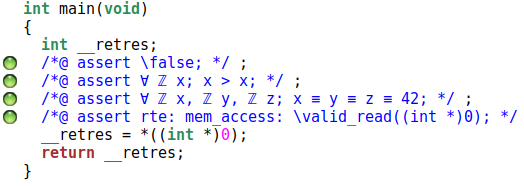
\includegraphics[scale=0.5]{false_axiom.png}
  \caption{Different false things proved to be true}
  \label{fig:false-axiom}
\end{figure}

Of course, this example is extreme, we would not write such an axiom.
The problem is in fact that it is really easy to write an axiomatic
definition that is subtly false when we express more complex properties,
or adding assumptions about the global state of the system.

When we start to create axiomatic definitions, it is worth adding
assertions or postconditions requiring a proof of false that we expect
to fail to ensure that the definition is not inconsistent. However, it
is often not enough! If the subtlety that creates the inconsistency is
hard enough to find, provers could need a lot of information other than
the axiomatic definition itself to be able to find and use the
inconsistency, we then need to always be careful!

More specifically, specifying the values read by a function or a
predicate is important for the consistency of an axiomatic definition.
Indeed, as previously explained, if we do not specify what is read when
a pointer is received, an update of a value inside the array do not
invalidate a property known about the content of the array. In such a
case, the proof is performed but since the axiom do not talk about the
content of the array, we do not prove anything.

For example, in the function that resets an array to 0, if we modify the
axiomatic definition, removing the specification of the values that are
read by the predicate (\texttt{reads\ a{[}b\ ..\ e-1{]}}), the proof
will still be performed, but will not prove anything about the content
of the arrays.

\subsection{Example: counting occurrences of a
value}\label{example-counting-occurrences-of-a-value}

In this example, we want to prove that an algorithm actually counts the
occurrences of a value inside an array. We start by axiomatically define
what is the number of occurrences of a value inside an array:

\begin{footnotesize}\begin{Shaded}
\begin{Highlighting}[]
\CommentTok{/*@}
\CommentTok{  axiomatic Occurrences_Axiomatic\{}
\CommentTok{    logic integer l_occurrences_of\{L\}(int value, int* in, integer from, integer to)}
\CommentTok{      reads in[from .. to-1];}

\CommentTok{    axiom occurrences_empty_range\{L\}:}
\CommentTok{      \textbackslash{}forall int v, int* in, integer from, to;}
\CommentTok{        from >= to ==> l_occurrences_of\{L\}(v, in, from, to) == 0;}

\CommentTok{    axiom occurrences_positive_range_with_element\{L\}:}
\CommentTok{      \textbackslash{}forall int v, int* in, integer from, to;}
\CommentTok{        (from < to && in[to-1] == v) ==>}
\CommentTok{      l_occurrences_of(v,in,from,to) == 1+l_occurrences_of(v,in,from,to-1);}

\CommentTok{    axiom occurrences_positive_range_without_element\{L\}:}
\CommentTok{      \textbackslash{}forall int v, int* in, integer from, to;}
\CommentTok{        (from < to && in[to-1] != v) ==>}
\CommentTok{      l_occurrences_of(v,in,from,to) == l_occurrences_of(v,in,from,to-1);}
\CommentTok{  \}}
\CommentTok{*/}
\end{Highlighting}
\end{Shaded}\end{footnotesize}

We have three different cases:

\begin{itemize}
\tightlist
\item
  the considered range of values is empty: the number of occurrences is
  0,
\item
  the considered range of values is not empty and the last element is
  the one we are searching: the number of occurrences is the number of
  occurrences in the current range without the last element, plus 1,
\item
  the considered range of values is not empty and the last element is
  not the one we are searching: the number of occurrences is the number
  of occurrences in the current range without the last element.
\end{itemize}

Then, we can write the C function that computes the number of
occurrences of a value inside an array and prove it:

\clearpage
\begin{footnotesize}\begin{Shaded}
\begin{Highlighting}[]
\CommentTok{/*@}
\CommentTok{  requires \textbackslash{}valid_read(in+(0 .. length));}
\CommentTok{  assigns  \textbackslash{}nothing;}
\CommentTok{  ensures  \textbackslash{}result == l_occurrences_of(value, in, 0, length);}
\CommentTok{*/}
\NormalTok{size_t occurrences_of(}\DataTypeTok{int} \NormalTok{value, }\DataTypeTok{int}\NormalTok{* in, size_t length)\{}
  \NormalTok{size_t result = }\DecValTok{0}\NormalTok{;}
  
  \CommentTok{/*@}
\CommentTok{    loop invariant 0 <= result <= i <= length;}
\CommentTok{    loop invariant result == l_occurrences_of(value, in, 0, i);}
\CommentTok{    loop assigns i, result;}
\CommentTok{    loop variant length-i;}
\CommentTok{  */}
  \KeywordTok{for}\NormalTok{(size_t i = }\DecValTok{0}\NormalTok{; i < length; ++i)}
    \NormalTok{result += (in[i] == value)? }\DecValTok{1} \NormalTok{: }\DecValTok{0}\NormalTok{;}

  \KeywordTok{return} \NormalTok{result;}
\NormalTok{\}}
\end{Highlighting}
\end{Shaded}\end{footnotesize}

An alternative way to specify, in this code, that \texttt{result} is at
most \texttt{i}, is to express a more general lemma about the number of
occurrences of a value inside an array, since we know that it is
comprised between 0 and the size of maximum considered range of values:

\begin{footnotesize}\begin{Shaded}
\begin{Highlighting}[]
\CommentTok{/*@}
\CommentTok{lemma l_occurrences_of_range\{L\}:}
\CommentTok{  \textbackslash{}forall int v, int* array, integer from, to:}
\CommentTok{    from <= to ==> 0 <= l_occurrences_of(v, a, from, to) <= to-from;}
\CommentTok{*/}
\end{Highlighting}
\end{Shaded}\end{footnotesize}

An automatic solver cannot discharge this lemma. It would be necessary
to prove it interactively using Coq, for example. By expressing, generic
manually proved lemmas, we can often add useful tools to provers to
manipulate more efficiently our axiomatic definitions, without directly
adding new axioms that would augment the chances to introduce errors.
Here, we still have to realize the proof of the lemma to have a complete
proof.

\subsection{Example: sort}\label{example-sort}

We will prove a simple selection sort:

\begin{footnotesize}\begin{Shaded}
\begin{Highlighting}[]
\NormalTok{size_t min_idx_in(}\DataTypeTok{int}\NormalTok{* a, size_t beg, size_t end)\{}
  \NormalTok{size_t min_i = beg;}
  \KeywordTok{for}\NormalTok{(size_t i = beg}\DecValTok{+1}\NormalTok{; i < end; ++i)}
    \KeywordTok{if}\NormalTok{(a[i] < a[min_i]) min_i = i;}
  \KeywordTok{return} \NormalTok{min_i;}
\NormalTok{\}}

\DataTypeTok{void} \NormalTok{swap(}\DataTypeTok{int}\NormalTok{* p, }\DataTypeTok{int}\NormalTok{* q)\{}
  \DataTypeTok{int} \NormalTok{tmp = *p; *p = *q; *q = tmp;}
\NormalTok{\}}

\DataTypeTok{void} \NormalTok{sort(}\DataTypeTok{int}\NormalTok{* a, size_t beg, size_t end)\{}
  \KeywordTok{for}\NormalTok{(size_t i = beg ; i < end ; ++i)\{}
    \NormalTok{size_t imin = min_idx_in(a, i, end);}
    \NormalTok{swap(&a[i], &a[imin]);}
  \NormalTok{\}}
\NormalTok{\}}
\end{Highlighting}
\end{Shaded}\end{footnotesize}

The reader can exercise by specifying and proving the search of the
minimum and the swap function. We hide there a correct version of these
specification and code, we will focus on the specification and the proof
of the sort function that is a interesting use case for axiomatic
definitions.

\begin{zdssecretblock}{Answer}
  \begin{footnotesize}
  \begin{footnotesize}\begin{Shaded}
\begin{Highlighting}[]
\CommentTok{/*@}
\CommentTok{  requires \textbackslash{}valid_read(a + (beg .. end-1));}
\CommentTok{  requires beg < end;}

\CommentTok{  assigns  \textbackslash{}nothing;}

\CommentTok{  ensures  \textbackslash{}forall integer i; beg <= i < end ==> a[\textbackslash{}result] <= a[i];}
\CommentTok{  ensures  beg <= \textbackslash{}result < end;}
\CommentTok{*/}
\NormalTok{size_t min_idx_in(}\DataTypeTok{int}\NormalTok{* a, size_t beg, size_t end)\{}
  \NormalTok{size_t min_i = beg;}

  \CommentTok{/*@}
\CommentTok{    loop invariant beg <= min_i < i <= end;}
\CommentTok{    loop invariant \textbackslash{}forall integer j; beg <= j < i ==> a[min_i] <= a[j];}
\CommentTok{    loop assigns min_i, i;}
\CommentTok{    loop variant end-i;}
\CommentTok{  */}
  \KeywordTok{for}\NormalTok{(size_t i = beg}\DecValTok{+1}\NormalTok{; i < end; ++i)\{}
    \KeywordTok{if}\NormalTok{(a[i] < a[min_i]) min_i = i;}
  \NormalTok{\}}
  \KeywordTok{return} \NormalTok{min_i;}
\NormalTok{\}}

\CommentTok{/*@}
\CommentTok{  requires \textbackslash{}valid(p) && \textbackslash{}valid(q);}
\CommentTok{  assigns  *p, *q;}
\CommentTok{  ensures  *p == \textbackslash{}old(*q) && *q == \textbackslash{}old(*p);}
\CommentTok{*/}
\DataTypeTok{void} \NormalTok{swap(}\DataTypeTok{int}\NormalTok{* p, }\DataTypeTok{int}\NormalTok{* q)\{}
  \DataTypeTok{int} \NormalTok{tmp = *p; *p = *q; *q = tmp;}
\NormalTok{\}}
\end{Highlighting}
  \end{Shaded}\end{footnotesize}
  \end{footnotesize}
\end{zdssecretblock}

Indeed, a common error we could do, trying to prove a sort function,
would be to write the (true!) specification illustrated by
Figure~\ref{fig:6-1-5-insuff}.

\begin{figure}
\begin{footnotesize}\begin{Shaded}
\begin{Highlighting}[]
\CommentTok{/*@}
\CommentTok{  predicate sorted(int* a, integer b, integer e) =}
\CommentTok{    \textbackslash{}forall integer i, j; b <= i <= j < e ==> a[i] <= a[j];}
\CommentTok{*/}

\CommentTok{/*@}
\CommentTok{  requires \textbackslash{}valid(a + (beg .. end-1));}
\CommentTok{  requires beg < end;}
\CommentTok{  assigns  a[beg .. end-1];}
\CommentTok{  ensures sorted(a, beg, end);}
\CommentTok{*/}
\DataTypeTok{void} \NormalTok{sort(}\DataTypeTok{int}\NormalTok{* a, size_t beg, size_t end)\{}
  \CommentTok{/*@ //annotation de l'invariant */}
  \KeywordTok{for}\NormalTok{(size_t i = beg ; i < end ; ++i)\{}
    \NormalTok{size_t imin = min_idx_in(a, i, end);}
    \NormalTok{swap(&a[i], &a[imin]);}
  \NormalTok{\}}
\NormalTok{\}}
\end{Highlighting}
\end{Shaded}\end{footnotesize}
\caption{Underspecified \texttt{sort} function}
\label{fig:6-1-5-insuff}
\end{figure}

\textbf{This specification is true}. But if we recall correctly the part
of the tutorial about specifications, we have to \emph{precisely}
express what we expect of the program. With this specification, we do
not prove all required properties expected for a sort function. For
example, the function presented in Figure~\ref{fig:6-1-5-sort-faux} correctly
answers to the specification:

\begin{figure}
\begin{footnotesize}\begin{Shaded}
\begin{Highlighting}[]
\CommentTok{/*@}
\CommentTok{  requires \textbackslash{}valid(a + (beg .. end-1));}
\CommentTok{  requires beg < end;}

\CommentTok{  assigns  a[beg .. end-1];}
\CommentTok{  }
\CommentTok{  ensures sorted(a, beg, end);}
\CommentTok{*/}
\DataTypeTok{void} \NormalTok{fail_sort(}\DataTypeTok{int}\NormalTok{* a, size_t beg, size_t end)\{}
  \CommentTok{/*@}
\CommentTok{    loop invariant beg <= i <= end;}
\CommentTok{    loop invariant \textbackslash{}forall integer j; beg <= j < i ==> a[j] == 0;}
\CommentTok{    loop assigns i, a[beg .. end-1];}
\CommentTok{    loop variant end-i;}
\CommentTok{  */}
  \KeywordTok{for}\NormalTok{(size_t i = beg ; i < end ; ++i)}
    \NormalTok{a[i] = }\DecValTok{0}\NormalTok{;}
\NormalTok{\}}
\end{Highlighting}
\end{Shaded}\end{footnotesize}
\caption{Function that satisfies the specification of Figure~\ref{fig:6-1-5-insuff}}
\label{fig:6-1-5-sort-faux}
\end{figure}

Our specification does not express the fact that all elements initially
found inside the array must still be found inside the array after
executing the sort function. That is to say: the sort function produces
a sorted permutation of the original array.

Defining the notion of permutation is easily done using an axiomatic
definition. Indeed, to determine that an array is the permutation of an
other one, we can limit us to a few cases. First, the array is a
permutation of itself, then swapping to values of the array produces a
new permutation if we do not change anything else. And finally if we
create the permutation \(p_2\) of \(p_1\), and then the permutation
\(p_3\) of \(p_2\), then by transitivity \(p_3\) is a permutation of
\(p_1\).

The corresponding axiomatic definition is the following:

\begin{footnotesize}\begin{Shaded}
\begin{Highlighting}[]
\CommentTok{/*@}
\CommentTok{  predicate swap_in_array\{L1,L2\}(int* a, integer b, integer e, integer i, integer j) =}
\CommentTok{    b <= i < e && b <= j < e &&}
\CommentTok{    \textbackslash{}at(a[i], L1) == \textbackslash{}at(a[j], L2) && \textbackslash{}at(a[j], L1) == \textbackslash{}at(a[i], L2) &&}
\CommentTok{    \textbackslash{}forall integer k; b <= k < e && k != j && k != i ==> \textbackslash{}at(a[k], L1) == \textbackslash{}at(a[k], L2);}

\CommentTok{  axiomatic Permutation\{}
\CommentTok{    predicate permutation\{L1,L2\}(int* a, integer b, integer e)}
\CommentTok{     reads \textbackslash{}at(*(a+(b .. e - 1)), L1), \textbackslash{}at(*(a+(b .. e - 1)), L2);}

\CommentTok{    axiom reflexive\{L1\}: }
\CommentTok{      \textbackslash{}forall int* a, integer b,e ; permutation\{L1,L1\}(a, b, e);}

\CommentTok{    axiom swap\{L1,L2\}:}
\CommentTok{      \textbackslash{}forall int* a, integer b,e,i,j ;}
\CommentTok{        swap_in_array\{L1,L2\}(a,b,e,i,j) ==> permutation\{L1,L2\}(a, b, e);}
\CommentTok{    }
\CommentTok{    axiom transitive\{L1,L2,L3\}:}
\CommentTok{      \textbackslash{}forall int* a, integer b,e ; }
\CommentTok{        permutation\{L1,L2\}(a, b, e) && permutation\{L2,L3\}(a, b, e) ==> permutation\{L1,L3\}(a, b, e);}
\CommentTok{  \}}
\CommentTok{*/}
\end{Highlighting}
\end{Shaded}\end{footnotesize}

We can then specify that our sort function produces the sorted
permutation of the original array and we can then prove it by providing
the invariant of the function:

\begin{footnotesize}\begin{Shaded}
\begin{Highlighting}[]
\CommentTok{/*@}
\CommentTok{  requires beg < end && \textbackslash{}valid(a + (beg .. end-1));}
\CommentTok{  assigns  a[beg .. end-1];  }
\CommentTok{  ensures sorted(a, beg, end);}
\CommentTok{  ensures permutation\{Pre, Post\}(a,beg,end);}
\CommentTok{*/}
\DataTypeTok{void} \NormalTok{sort(}\DataTypeTok{int}\NormalTok{* a, size_t beg, size_t end)\{}
  \CommentTok{/*@}
\CommentTok{    loop invariant beg <= i <= end;}
\CommentTok{    loop invariant sorted(a, beg, i) && permutation\{Begin, Here\}(a, beg, end);}
\CommentTok{    loop invariant \textbackslash{}forall integer j,k; beg <= j < i ==> i <= k < end ==> a[j] <= a[k];}
\CommentTok{    loop assigns i, a[beg .. end-1];}
\CommentTok{    loop variant end-i;}
\CommentTok{  */}
  \KeywordTok{for}\NormalTok{(size_t i = beg ; i < end ; ++i)\{}
    \CommentTok{//@ ghost begin: ;}
    \NormalTok{size_t imin = min_idx_in(a, i, end);}
    \NormalTok{swap(&a[i], &a[imin]);}
    \CommentTok{//@ assert swap_in_array\{begin,Here\}(a,beg,end,i,imin);}
  \NormalTok{\}}
\NormalTok{\}}
\end{Highlighting}
\end{Shaded}\end{footnotesize}

This time, our property is precisely defined, the proof is relatively
easy to produce, only requiring to add an assertion in the block of the
loop to state that it only performs a swap of values inside the array
(and then giving the transition to the next permutation). To define this
swap notion, we use a particular annotation (at line 16), introduced
using the keyword \texttt{ghost}. Here, the goal is to introduce a label
in the code that in fact does not exists from the program point of view,
and is only visible from a specification point of view. This is the
topic of the next section.

\section{Ghost code}\label{ghost-code}

Behind this title, that seems to be an action movie, we find in fact a
way to enrich our specification with information expressed as regular C
code. Here, the idea is to add variables and source code that will not
be part of the actual program but will model logic states that will only
be visible from a proof point of view. Using it, we can make explicit
some logic properties that were previously only known implicitly.

\subsection{Syntax}\label{syntax-4}

Ghost code is added using annotations that will contains C code
introduced using the \texttt{ghost} keyword:

\begin{footnotesize}\begin{Shaded}
\begin{Highlighting}[]
\CommentTok{/*@}
\CommentTok{  ghost}
\CommentTok{  // C source code}
\CommentTok{*/}
\end{Highlighting}
\end{Shaded}\end{footnotesize}

The only rules we have to respect in such a code, is that we cannot
write a memory block that is not itself defined in ghost code, and that
the code must close any block it would open. Apart of this, any
computation can be inserted provided it \emph{only} modifies ghost
variables.

Here are some examples of ghost code:

\begin{footnotesize}\begin{Shaded}
\begin{Highlighting}[]
\CommentTok{//@ ghost int ghost_glob_var = 0;}

\DataTypeTok{void} \NormalTok{foo(}\DataTypeTok{int} \NormalTok{a)\{}
  \CommentTok{//@ ghost int ghost_loc_var = a;}

  \CommentTok{//@ ghost Ghost_label: ;}
  \NormalTok{a = }\DecValTok{28} \NormalTok{;}

  \CommentTok{//@ ghost if(a < 0)\{ ghost_loc_var = 0; \}}

  \CommentTok{//@ assert ghost_loc_var == \textbackslash{}at(a, Ghost_label) == \textbackslash{}at(a, Pre);}
\NormalTok{\}}
\end{Highlighting}
\end{Shaded}\end{footnotesize}

We must again be careful using ghost code. Indeed, the tool will not
perform any verification to ensure that we do not write in the memory of
the program by mistake. This problem being, in fact, an undecidable
problem, this analysis would require a proof by itself. For example,
this code is allowed in input of Frama-C even if it explicitly modifies
the state of the program we want to verify:

\begin{footnotesize}\begin{Shaded}
\begin{Highlighting}[]
\DataTypeTok{int} \NormalTok{a;}

\DataTypeTok{void} \NormalTok{foo()\{}
  \CommentTok{//@ ghost a = 42;}
\NormalTok{\}}
\end{Highlighting}
\end{Shaded}\end{footnotesize}

We then need to be really careful about we are doing using ghost code
(by making it simple).

\subsection{Make a logical state
explicit}\label{make-a-logical-state-explicit}

The goal of ghost code is to make explicit some information that are
without them implicit. For example, in the previous section, we used it
to get an explicit logic state known at a particular point of the
program.

Let us take a more complex example. Here, we want to prove that the
following function returns the value of the maximal sum of subarrays of
a given array. A subarray of an array \texttt{a} is a contiguous subset
of values of \texttt{a}. For example, for an array
\texttt{\{\ 0\ ,\ 3\ ,\ -1\ ,\ 4\ \}}, some subarrays can be
\texttt{\{\}}, \texttt{\{\ 0\ \}}, \texttt{\{\ 3\ ,\ -1\ \}},
\texttt{\{\ 0\ ,\ 3\ ,\ -1\ ,\ 4\ \}}, \ldots{} Note that as we allow
empty arrays for subarrays, the sum is at least 0. In the previous
array, the subarray with the maximal sum is
\texttt{\{\ 3\ ,\ -1\ ,\ 4\ \}}, the function would then return 6.

\begin{footnotesize}\begin{Shaded}
\begin{Highlighting}[]
\DataTypeTok{int} \NormalTok{max_subarray(}\DataTypeTok{int} \NormalTok{*a, size_t len) \{}
  \DataTypeTok{int} \NormalTok{max = }\DecValTok{0}\NormalTok{;}
  \DataTypeTok{int} \NormalTok{cur = }\DecValTok{0}\NormalTok{;}
  \KeywordTok{for}\NormalTok{(size_t i = }\DecValTok{0}\NormalTok{; i < len; i++) \{}
    \NormalTok{cur += a[i];}
    \KeywordTok{if} \NormalTok{(cur < }\DecValTok{0}\NormalTok{)   cur = }\DecValTok{0}\NormalTok{;}
    \KeywordTok{if} \NormalTok{(cur > max) max = cur;}
  \NormalTok{\}}
  \KeywordTok{return} \NormalTok{max;}
\NormalTok{\}}
\end{Highlighting}
\end{Shaded}\end{footnotesize}

In order to specify the previous function, we will need an axiomatic
definition about sum. This is not too much complex, the careful reader
can express the needed axioms as an exercise:

\begin{footnotesize}\begin{Shaded}
\begin{Highlighting}[]
\CommentTok{/*@ axiomatic Sum \{}
\CommentTok{  logic integer sum(int *array, integer begin, integer end) reads a[begin..(end-1)];}
\CommentTok{\}*/}
\end{Highlighting}
\end{Shaded}\end{footnotesize}

Some correct axioms are hidden there:

\begin{zdssecretblock}{Answer}
\begin{footnotesize}\begin{Shaded}
\begin{Highlighting}[]
\CommentTok{/*@}
\CommentTok{  axiomatic Sum_array\{}
\CommentTok{    logic integer sum(int* array, integer begin, integer end) }
\CommentTok{      reads array[begin .. (end-1)];}
\CommentTok{   }
\CommentTok{    axiom empty: }
\CommentTok{      \textbackslash{}forall int* a, integer b, e; b >= e ==> sum(a,b,e) == 0;}
\CommentTok{    axiom range:}
\CommentTok{      \textbackslash{}forall int* a, integer b, e; b < e ==> sum(a,b,e) == sum(a,b,e-1)+a[e-1];}
\CommentTok{  \}}
\CommentTok{*/}
\end{Highlighting}
\end{Shaded}\end{footnotesize}
\end{zdssecretblock}

The specification of the function is the following:

\begin{footnotesize}\begin{Shaded}
\begin{Highlighting}[]
\CommentTok{/*@ }
\CommentTok{  requires \textbackslash{}valid(a+(0..len-1));}
\CommentTok{  assigns \textbackslash{}nothing;}
\CommentTok{  ensures \textbackslash{}forall integer l, h;  0 <= l <= h <= len ==> sum(a,l,h) <= \textbackslash{}result;}
\CommentTok{  ensures \textbackslash{}exists integer l, h;  0 <= l <= h <= len &&  sum(a,l,h) == \textbackslash{}result;}
\CommentTok{*/}
\end{Highlighting}
\end{Shaded}\end{footnotesize}

For any bounds, the value returned by the function must be greater or
equal to the sum of the elements between these bounds, and there must
exist some bounds such that the returned value is exactly the sum of the
elements between these bounds. About this specification, when we want to
add the loop invariant, we will realize that we miss some information.
We want to express what are the values \texttt{max} and \texttt{cur} and
what are the relations between them, but we cannot do it!

Basically, our postcondition needs to know that there exists some bounds
\texttt{low} and \texttt{high} such that the computed sum corresponds to
these bounds. However, in our code, we do not have anything that express
it from a logic point of view, and we cannot \emph{a priori} make the
link between this logical formalization. We will then use ghost code to
record these bounds and express the loop invariant.

We will first need two variables that will allow us to record the bounds
of the maximum sum range, we will call them \texttt{low} and
\texttt{high}. Every time we will find a range where the sum is greater
than the current one, we will update our ghost variables. This bounds
will then corresponds to the sum currently stored by \texttt{max}. That
induces that we need other bounds: the ones that corresponds to the sum
store by the variable \texttt{cur} from which we will build the bounds
corresponding to \texttt{max}. For these bounds, we will only add a
single ghost variable: the current low bound \texttt{cur\_low}, the high
bound being the variable \texttt{i} of the loop. The specified code is
illustrated by Figure~\ref{fig:6-2-2-maxsub}.

\begin{figure}
\begin{footnotesize}\begin{Shaded}
\begin{Highlighting}[]
\CommentTok{/*@ }
\CommentTok{  requires \textbackslash{}valid(a+(0..len-1));}
\CommentTok{  assigns \textbackslash{}nothing;}
\CommentTok{  ensures \textbackslash{}forall integer l, h;  0 <= l <= h <= len ==> sum(a,l,h) <= \textbackslash{}result;}
\CommentTok{  ensures \textbackslash{}exists integer l, h;  0 <= l <= h <= len &&  sum(a,l,h) == \textbackslash{}result;}
\CommentTok{*/}
\DataTypeTok{int} \NormalTok{max_subarray(}\DataTypeTok{int} \NormalTok{*a, size_t len) \{}
  \DataTypeTok{int} \NormalTok{max = }\DecValTok{0}\NormalTok{;}
  \DataTypeTok{int} \NormalTok{cur = }\DecValTok{0}\NormalTok{;}
  \CommentTok{//@ ghost size_t cur_low = 0; }
  \CommentTok{//@ ghost size_t low = 0;}
  \CommentTok{//@ ghost size_t high = 0; }

  \CommentTok{/*@ }
\CommentTok{    loop invariant BOUNDS: low <= high <= i <= len && cur_low <= i;}
\CommentTok{    }
\CommentTok{    loop invariant REL :   cur == sum(a,cur_low,i) <= max == sum(a,low,high);}
\CommentTok{    loop invariant POST:   \textbackslash{}forall integer l;    0 <= l <= i      ==> sum(a,l,i) <= cur;}
\CommentTok{    loop invariant POST:   \textbackslash{}forall integer l, h; 0 <= l <= h <= i ==> sum(a,l,h) <= max;}
\CommentTok{   }
\CommentTok{    loop assigns i, cur, max, cur_low, low, high;}
\CommentTok{    loop variant len - i; }
\CommentTok{  */}
  \KeywordTok{for}\NormalTok{(size_t i = }\DecValTok{0}\NormalTok{; i < len; i++) \{}
    \NormalTok{cur += a[i];}
    \KeywordTok{if} \NormalTok{(cur < }\DecValTok{0}\NormalTok{) \{}
      \NormalTok{cur = }\DecValTok{0}\NormalTok{;}
      \CommentTok{/*@ ghost cur_low = i+1; */}
    \NormalTok{\}}
    \KeywordTok{if} \NormalTok{(cur > max) \{}
      \NormalTok{max = cur;}
      \CommentTok{/*@ ghost low = cur_low; */}
      \CommentTok{/*@ ghost high = i+1; */}
    \NormalTok{\}}
  \NormalTok{\}}
  \KeywordTok{return} \NormalTok{max;}
\NormalTok{\}}
\end{Highlighting}
\end{Shaded}\end{footnotesize}
\caption{Specified \texttt{max\_sub\_array} function}
\label{fig:6-2-2-maxsub}
\end{figure}

The invariant \texttt{BOUNDS} expresses how the different bounds are
ordered during the computation. The invariant \texttt{REL} expresses
what the variables \texttt{cur} and \texttt{max} mean depending on the
bounds. Finally, the invariant \texttt{POST} allows us to create a link
between the invariant and the postcondition of the function.

The reader can verify that this function is indeed correctly proved
without RTE verification. If we add RTE verification, the overflow on
the variable \texttt{cur}, that is the sum, seems to be possible (and it
is indeed the case).

Here, we will not try to fix this because it is not the topic of this
example. The way we can prove the absence of RTE here strongly depends
on the context where we use this function. A possibility is to strongly
restrict the contract, forcing some properties about values and the size
of the array. For example, we could strongly limit the maximal size of
the array and strong bounds on each value of the different cells. An
other possibility would be to add an error value in case of overflow
(\(-1\) for example), and to specify that when an overflow is produced,
this value is returned.

In this part, we have covered some advanced constructions of the ACSL
language that allows to express and prove more complex properties about
programs.

Badly used, this features can make our analyses incorrect, we then need
to be careful manipulating them and not hesitate to check them again and
again, or eventually express properties to verify about them to assure
that we are not introducing an incoherence in our program or our
assumptions.

\chapter{Conclusion}\label{conclusion}

\begin{quote}
Voilà, c'est fini \ldots{} \hfill {[}Jean-Louis Aubert, \emph{Bleu Blanc
Vert}, 1989{]}
\end{quote}

\ldots{} for this introduction to the proof of C programs using Frama-C
and WP.

Along this tutorial, we have seen how we can use these tools to specify
what we except of our programs and verify that the source code we have
produced indeed corresponds to the specification we have provided. This
specification is provided using annotations of our functions that
includes the contract they must respect. These contracts are properties
required about the input to ensure that the function will correctly
work, which is specified by properties about the output of the function.

Starting from specified programs, WP is able to produce the weakest
precondition of our programs, provided what we want in postcondition,
and to ask some provers if the specified precondition is compatible with
the computed one. The reasoning is completely modular, which allows to
prove function in isolation from each other and to compose the results.
WP cannot currently work with dynamic allocation. A function that would
use it could not be proved.

However, even without dynamic allocation, a lot of function can be
proved since they work with data-structures that are already allocated.
And these functions can then be called with the certainty that they
perform a correct job. If we cannot or do not want to prove calling
code, we can still write something like this:

\begin{footnotesize}\begin{Shaded}
\begin{Highlighting}[]
\CommentTok{/*@}
\CommentTok{  requires some_properties_on(a);}
\CommentTok{  requires some_other_on(b);}

\CommentTok{  assigns ...}
\CommentTok{  ensures ...}
\CommentTok{*/}
\DataTypeTok{void} \NormalTok{ma_fonction(}\DataTypeTok{int}\NormalTok{* a, }\DataTypeTok{int} \NormalTok{b)\{}
  \CommentTok{//this is indeed the "assert" defined in "assert.h"}
  \NormalTok{assert(}\CommentTok{/*properties on a*/} \NormalTok{&& }\StringTok{"must respect properties on a"}\NormalTok{);  }
  \NormalTok{assert(}\CommentTok{/*properties on b*/} \NormalTok{&& }\StringTok{"must respect properties on b"}\NormalTok{);}
\NormalTok{\}}
\end{Highlighting}
\end{Shaded}\end{footnotesize}

Which allows us to benefit from the robustness of our function having
the possibility to debug and incorrect call in a source code that we
cannot or do want to prove.

Writing specifications is sometimes long or tedious. Higher-level
features of ACSL (predicates, logic functions, axiomatizations) allow us
to lighten this work, as well as our programming languages allow us to
define types containing other types, functions call functions, bringing
us to the final program. But, despite this, write specification in a
formal language, no matter which one, is generally a hard task.

However, this \textbf{formalization} of our need is \textbf{crucial}.
Concretely, such a formalization is a work every developer should do.
And not only in order to prove a program. Even the definition of tests
for a function requires to correctly understand its goal if we want to
test what is necessary and only what is necessary. And writing
specification in a formal language is incredibly useful (even if it can
be sometimes frustrating) to get a clear specification.

Formal languages, that are close to mathematics, are precise.
Mathematics have this: they are precise. What is more terrible that
reading a specification written in a natural language, with complex
sentences, using conditional forms, imprecise terms, ambiguities,
compiled in administrative documents composed of hundreds of pages, and
where we need to determine, ``so, what this function is supposed to do ?
And have I to validate about it ?''.

Formal methods are probably not enough used currently. Sometimes because
of mistrust, sometimes because of ignorance, sometimes becuase of
prejudices based on ideas born at the begining of the tools, 20 years
ago. Our tools evolve, the way we develop change, probably faster than
in any other technical domain. Saying that these tools could never be
used for real life programs would certainly be a too big shortcut. After
all, we see everyday how much development is different from what it were
10 years, 20 years, 40 years ago and can barely imagine how much it will
be different in 10 years, 20 years, 40 years.

During the past few years, safety and security questions have become
more and more actual and crucial. Formal methods also progressed a lot,
and the improvement they bring for these questions are greatly
appreciated. For example, this
\href{http://sfm.seas.harvard.edu/report.html}{hyperlink} brings to the
report of a conference about security that brought together people from
academic and industrial world, in which we can read:

\begin{quote}
Adoption of formal methods in various areas (including verification of
hardware and embedded systems, and analysis and testing of software) has
dramatically improved the quality of computer systems. We anticipate
that formal methods can provide similar improvement in the security of
computer systems.

{[}\ldots{}{]}

\textbf{Without broad use of formal methods, security will always remain
fragile.} \hfill{[}Formal Methods for Security, 2016{]}
\end{quote}

\chapter{Going further}\label{going-further}

\section{With Frama-C}\label{with-frama-c}

Frama-C provides different ways to analyse programs. In these tools, the
most commonly used and interesting to know from a static and dynamic
verification point of view are certainly those ones:

\begin{itemize}
\tightlist
\item
  abstract interpretation analysis using
  \href{http://frama-c.com/value.html}{EVA},
\item
  the transformation of annotation into runtime verification using
  \href{http://frama-c.com/eacsl.html}{E-ACSL}.
\end{itemize}

The goal of the first one is to compute the domain of the different
variables at each program point. When we precisely know these domains,
we can determine if these variables can produce errors when they are
used. However this analysis is executed on the whole program and not
modularly, it is also stongly dependent of the type of domain we use (we
will not enter into details here) and it is not so good at keeping the
relations between variables. On the other side, it is really completely
automatic, we do not even need to give loop invariant ! The most manual
part of the work is to determine whether or not an alarm is a true error
or a false positive.

The second analysis allows to generate from an original program, a new
program where the assertions are transformed into runtime verifications.
If these assertions fail, the program fails. If they are valid, the
program have the same behavior it would have without the assertions. An
example of use is to generate the verification of absence of runtime
errors as assertions using \texttt{-rte} and then to use E-ACSL to
generate the program containing the runtime verification that these
assertions do not fail.

There exists different other plugins for very different tasks:

\begin{itemize}
\tightlist
\item
  impact analysis of a modification,
\item
  data-flow analysis to visit it efficiently,
\item
  \ldots{}
\end{itemize}

Finally, a last possibility that will motivate the use of Frama-C is the
ability to develop their own analysis plugins using the API provided by
the Frama-C kernel. A lot of tasks can be realized by the analysis of
the source code and Frama-C allows to build different analyses.

\section{With deductive proof}\label{with-deductive-proof}

Along this tutorial we used WP to generate proof obligation starting
from programs with their specification. Next we have used automatic
solvers to assure that these properties were indeed verified.

When we use other solvers than Alt-Ergo and Coq, the communication with
this solver in provided by a translation to the Why3 language that will
next be used to bridge the gap to automatic solvers. But this is not the
only way to use Why3. It can also be used itself to write programs and
prove them. It especially provides a set of theories for some common
data structures.

There is some proofs that cannot be discharged by automatic solvers. In
such a case, we have to provide these proofs interactively. WP, like
Why3, can extract its goals to Coq, and it is very interesting to study
this language. In the context of Frama-C, we produce lemmas libraries
already proved that we can reuse. But Coq can also be used for many
different tasks, including programming. Note that Why3 can also extract
its proof obligations to Isabelle or PVS that are also proof assistants.

Finally, there exists other program logics, for example separation logic
or concurrent program logics. Again this notion are interesting to know
in the context of Frama-C: if we cannot directly use them, they can
inspire the way we specify our program in Frama-C for the proof with WP.
They could also be implemented into new plugins to Frama-C.

A whole new world of methods to explore.

\end{document}
